% Standalone wrapper for compiling the chapter on its own.
% In the full book, copy the package list into the book preamble and % Chapter 13: rare variants.
% Requires: amsmath, amssymb, bm, graphicx, booktabs, multirow, subcaption,
% tikz (arrows.meta, positioning, calc, decorations.pathreplacing, shapes.geometric, fit), natbib.
% Computed figures are produced by scripts/make_figures.py;
% figures/slides/ holds figures taken from the lecture slides.

\providecommand{\R}{\mathbb{R}}
\providecommand{\E}{\mathbb{E}}
\providecommand{\Normal}{\mathcal{N}}
\providecommand{\argmax}{\operatorname*{arg\,max}}
\providecommand{\argmin}{\operatorname*{arg\,min}}
\providecommand{\vy}{\mathbf{y}}
\providecommand{\vx}{\mathbf{x}}
\providecommand{\mX}{\mathbf{X}}
\providecommand{\mI}{\mathbf{I}}
\providecommand{\vb}{\boldsymbol{\beta}}
\providecommand{\veps}{\boldsymbol{\epsilon}}
\providecommand{\vp}{\mathbf{p}}
\providecommand{\vg}{\mathbf{g}}
\providecommand{\ind}{\mathbf{1}}
\providecommand{\valpha}{\boldsymbol{\alpha}}
\providecommand{\vz}{\mathbf{z}}
\providecommand{\va}{\mathbf{a}}
\providecommand{\vr}{\mathbf{r}}
\providecommand{\vmu}{\boldsymbol{\mu}}
\providecommand{\vphi}{\boldsymbol{\phi}}
\providecommand{\vw}{\mathbf{w}}
\providecommand{\vd}{\mathbf{d}}
\providecommand{\vc}{\mathbf{c}}
\providecommand{\vS}{\mathbf{S}}
\providecommand{\mG}{\mathbf{G}}
\providecommand{\mK}{\mathbf{K}}
\providecommand{\mW}{\mathbf{W}}
\providecommand{\mR}{\mathbf{R}}
\providecommand{\mP}{\mathbf{P}}
\providecommand{\mD}{\mathbf{D}}
\providecommand{\mV}{\mathbf{V}}
\providecommand{\mSigma}{\boldsymbol{\Sigma}}
\providecommand{\Var}{\operatorname{Var}}
\providecommand{\Cov}{\operatorname{Cov}}
\providecommand{\tr}{\operatorname{tr}}
\providecommand{\Bin}{\operatorname{Binomial}}
\providecommand{\BetaD}{\operatorname{Beta}}
\providecommand{\Pois}{\operatorname{Poisson}}

\chapter{Rare variants}
\label{ch:rare_variants}

Chapters 11 and 12 tested genetic variants one at a time for association with a disease, a quantitative trait or a molecular phenotype such as gene expression. That approach works for common variants, those whose minor allele is carried by at least a few percent of people. Most human genetic variants are rare, however, and some of the variants with the largest effects on disease are rare because natural selection keeps them that way. For variants carried by a handful of people, and for \emph{de novo} mutations, which are present in a single individual, a single-variant test has little or no power.

This chapter covers the methods developed for this setting. They rest on two ideas. The first is to aggregate: instead of testing each variant, test whether a gene or region carries more, or more damaging, variation in cases than in controls. This gives burden tests and the variance component tests SKAT and SKAT-O. The second is to use prior information about which variants are likely to matter. Pathogenicity predictors such as LINSIGHT, which learns from patterns of natural selection, and the deep learning models of regulatory sequence from Chapters 2 and 3 provide such information, and the functional score test and DeepRVAT build it into the association test. A case study of noncoding de novo mutations in autism shows these pieces used together, followed by network-based pathway analysis and experimental validation. The chapter ends with molecular data from patients: RNA-seq can reveal the consequences of a rare variant directly, as an expression, splicing or allelic outlier.

%======================================================================
\section{Why rare variants need different methods}
\label{sec:why_rare}
%======================================================================

\subsection{The allele frequency spectrum}

Recall from Chapter 11 that two unrelated people differ at roughly one position in every thousand. Each variable position, or single nucleotide polymorphism (SNP), usually has two alleles, and the \emph{minor allele frequency} (MAF) $f\in(0,0.5]$ is the frequency of the less common one. About three million SNPs per genome have $f\geq 5\%$ and are called common. Many more variants are rare. When large numbers of people are sequenced, the number of distinct variants keeps growing, and most newly found variants are seen in only one or a few individuals. The Genome Aggregation Database (gnomAD), which aggregated exome and genome sequences from 141,456 people~\citep{karczewski2020}, illustrates this: most of the variants it catalogues are rare, and a large fraction are \emph{singletons}, observed in a single person. A \emph{private} variant is found only in one family, and a \emph{de novo} mutation arose in a parent's germ cell, so that the child carries it and neither parent does. A typical genome carries around 70 de novo single nucleotide mutations.

\subsection{Effect size and allele frequency}

Effect sizes and allele frequencies are inversely related (Figure~\ref{fig:effect_freq})~\citep{manolio2009}. The variants that cause Mendelian diseases are rare and have large effects. The variants found by genome-wide association studies (GWAS) of common diseases are common and have small effects, with odds ratios typically below 1.5. Between these lie low-frequency variants of intermediate effect. Few common variants have large effects on common disease, and rare variants with small effects are very hard to find by genetic means at all.

The inverse relationship arises through natural selection. A variant that increases the risk of a disease that reduces the number of children its carriers have is selected against, and the stronger its effect, the more effectively selection keeps its frequency low. A variant of small effect is almost invisible to selection and can drift to high frequency. An exception is late-onset disease. Selection is blind to effects after reproductive age, which is one reason why alleles such as the \textit{APOE} $\varepsilon4$ allele, which increases the risk of Alzheimer's disease, remain common.

\begin{figure}[!htbp]
  \centering
  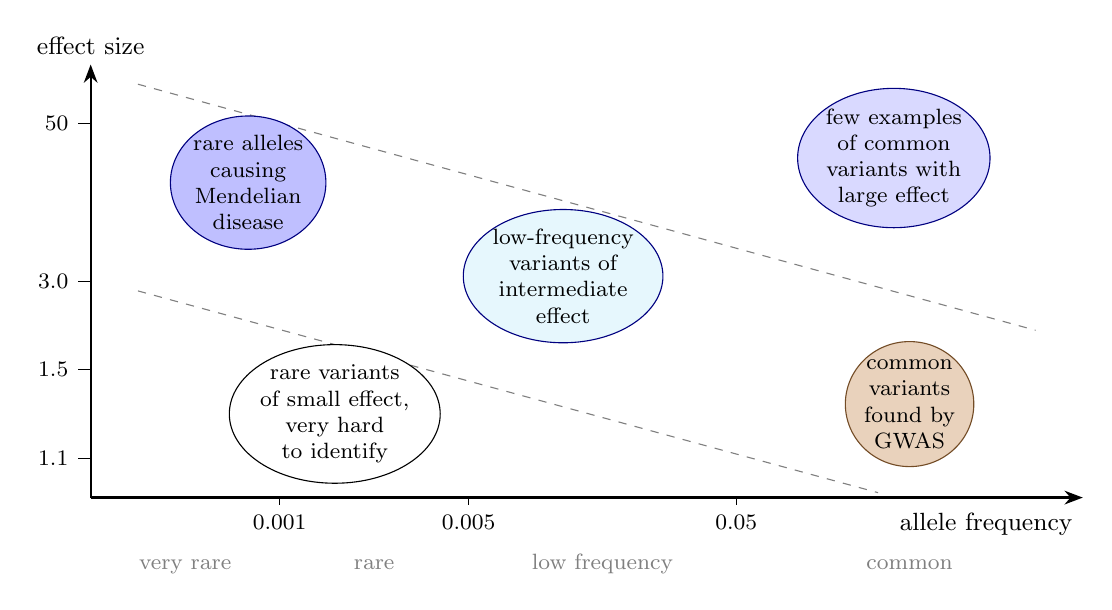
\begin{tikzpicture}[>=Stealth, every node/.style={font=\small}, x=2.0cm, y=1.25cm]
    \draw[->, thick] (0,0) -- (6.3,0) node[below left=2pt and 0pt, align=right] {allele frequency};
    \draw[->, thick] (0,0) -- (0,4.4) node[above] {effect size};
    \foreach \x/\l in {1.2/0.001, 2.4/0.005, 4.1/0.05} {
      \draw (\x,0) -- (\x,-0.08) node[below] {\footnotesize \l};
    }
    \node[below, font=\footnotesize, gray, text height=1.5ex, text depth=.25ex] at (0.6,-0.45) {very rare};
    \node[below, font=\footnotesize, gray, text height=1.5ex, text depth=.25ex] at (1.8,-0.45) {rare};
    \node[below, font=\footnotesize, gray, text height=1.5ex, text depth=.25ex] at (3.25,-0.45) {low frequency};
    \node[below, font=\footnotesize, gray, text height=1.5ex, text depth=.25ex] at (5.2,-0.45) {common};
    \foreach \y/\l in {0.4/1.1, 1.3/1.5, 2.2/3.0, 3.8/50} {
      \draw (0,\y) -- (-0.08,\y) node[left] {\footnotesize \l};
    }
    \draw[dashed, gray] (0.3,4.2) -- (6.0,1.7);
    \draw[dashed, gray] (0.3,2.1) -- (5.0,0.05);
    \tikzset{blob/.style={ellipse, draw, align=center, font=\footnotesize, inner sep=0pt}}
    \node[blob, fill=blue!25, draw=blue!50!black] at (1.0,3.2) {rare alleles\\causing\\Mendelian\\disease};
    \node[blob, fill=cyan!10, draw=blue!50!black] at (3.0,2.25) {low-frequency\\variants of\\intermediate\\effect};
    \node[blob, fill=brown!35, draw=brown!60!black] at (5.2,0.95) {common\\variants\\found by\\GWAS};
    \node[blob, fill=blue!15, draw=blue!50!black] at (5.1,3.45) {few examples\\of common\\variants with\\large effect};
    \node[blob, fill=white, draw=black] at (1.55,0.85) {rare variants\\of small effect,\\very hard\\to identify};
  \end{tikzpicture}
  \caption{Effect size (odds ratio, log scale) against risk allele frequency. Most known associations lie between the dashed lines. Redrawn after \citet{manolio2009}.}
  \label{fig:effect_freq}
\end{figure}

\subsection{Power of a single-variant test}
\label{sec:power}

Consider a quantitative trait and a single variant. Let $N$ be the number of individuals, $g_i\in\{0,1,2\}$ the number of copies of the minor allele carried by individual $i$, and $y_i\in\R$ the trait. The additive model from Chapter 11 is
\begin{equation}
  y_i = \mu + \beta g_i + \epsilon_i, \qquad \epsilon_i\overset{\text{iid}}{\sim}\Normal(0,\sigma^2),
\end{equation}
with intercept $\mu$, per-allele effect $\beta\in\R$ and noise variance $\sigma^2$. The least-squares estimate is $\hat\beta=\sum_i(g_i-\bar g)(y_i-\bar y)/\sum_i(g_i-\bar g)^2$, with variance $\sigma^2/\sum_i(g_i-\bar g)^2$. Under Hardy-Weinberg equilibrium $g_i\sim\Bin(2,f)$, so $\Var(g_i)=2f(1-f)$ and $\sum_i(g_i-\bar g)^2\approx 2Nf(1-f)$. The test statistic $z=\hat\beta/\operatorname{se}(\hat\beta)$ is then approximately normal with unit variance and mean
\begin{equation}
  \E[z] \approx \frac{\beta}{\sigma}\sqrt{2Nf(1-f)} .
  \label{eq:ncp}
\end{equation}
For a two-sided test at level $\alpha$ with critical value $z_{\alpha/2}$, the power, the probability of detecting the association when it is real, is
\begin{equation}
  \text{power} = \Phi\left(\E[z]-z_{\alpha/2}\right) + \Phi\left(-\E[z]-z_{\alpha/2}\right),
\end{equation}
where $\Phi$ is the standard normal cumulative distribution function. For rare variants $1-f\approx 1$, so power depends on the sample size and allele frequency only through $Nf$, which is half the expected number of minor alleles in the sample, and on the standardized effect $\beta/\sigma$. Halving the allele frequency requires doubling the sample size for the same power.

Figure~\ref{fig:power_single} shows the consequence at the genome-wide threshold $\alpha=5\times10^{-8}$. With $10^5$ individuals, a variant with a large effect, half a standard deviation per allele, is detected reliably down to a MAF of about $10^{-3}$, but a variant with a modest effect of $0.1\sigma$ needs a MAF of a few percent. Variants with $f=10^{-5}$ are out of reach even with a million people. For a de novo mutation, $Nf$ is effectively one: the variant is carried by one person, and no sample size will make a single-variant test informative.

\begin{figure}[!htbp]
  \centering
  \includegraphics[width=0.9\linewidth]{power_single_variant.pdf}
  \caption{Power of a single-variant additive test at $\alpha=5\times10^{-8}$ as a function of MAF, for sample sizes from $10^3$ to $10^6$ and two standardized effect sizes. Power depends on $N$ and $f$ through approximately $Nf$, so the curves are shifted copies on the log scale. Computed from~\eqref{eq:ncp}.}
  \label{fig:power_single}
\end{figure}

Two strategies follow. Since we cannot test each rare variant on its own, we \emph{aggregate} variants within a unit, usually a gene, and test the unit. And since aggregation dilutes the signal with neutral variants, we use \emph{prior information} to pick out, or upweight, the variants likely to be functional.

%======================================================================
\section{Burden tests}
\label{sec:burden}
%======================================================================

A burden test asks whether a gene carries more variants, or more damaging variants, in affected individuals than expected by chance. Let a gene or region contain $M$ variants that pass some filter, for example $f_j<1\%$ and a predicted loss of function. Let $\mG\in\{0,1,2\}^{N\times M}$ be the genotype matrix, with $G_{ij}$ the number of minor alleles of variant $j$ carried by individual $i$, and let $\vw\in\R^M_{\geq 0}$ be a vector of variant weights. The \emph{burden score} of individual $i$ is
\begin{equation}
  C_i = \sum_{j=1}^M w_j G_{ij} .
\end{equation}
Early versions collapse the variants into an indicator of carrying any qualifying variant, $C_i=\ind[\sum_j G_{ij}>0]$~\citep{morgenthaler2007, li2008}, or weight each variant by $w_j=1/\sqrt{f_j(1-f_j)}$, so that rarer variants count for more~\citep{madsen2009}. The burden score then replaces the genotype in a regression. With covariates $\vx_i\in\R^{C}$ (for example age, sex and genetic principal components), coefficients $\valpha\in\R^C$ and mean $\mu_i=\E[y_i]$,
\begin{equation}
  h(\mu_i) = \vx_i^\top\valpha + C_i\beta ,
  \label{eq:burden_glm}
\end{equation}
where $h$ is the identity for a quantitative trait and the logit for a binary trait. The test of $H_0:\beta=0$ is a single-degree-of-freedom test, so it is as cheap as testing one common variant.

The burden model is the per-variant model $h(\mu_i)=\vx_i^\top\valpha+\sum_j G_{ij}\beta_j$ with the constraint $\beta_j=w_j\beta$. It assumes that every qualifying variant has an effect, in the same direction, of size proportional to its weight. When this holds, pooling the variants concentrates their signal into one statistic. When it does not, the test loses power: neutral variants add noise to $C_i$, and variants with opposite effects cancel.

\subsection{The score test}

The tests in this chapter are \emph{score tests}, which need only the model fitted under the null hypothesis. For a quantitative trait, fit $y_i=\vx_i^\top\valpha+\epsilon_i$ by least squares and let $\hat\mu_i=\vx_i^\top\hat\valpha$ be the fitted values. The score for $\beta$ at $\beta=0$ is the derivative of the log likelihood, $\sigma^{-2}\sum_i C_i(y_i-\hat\mu_i)$. Define the score statistic of variant $j$ as
\begin{equation}
  S_j = \sum_{i=1}^N G_{ij}(y_i-\hat\mu_i), \qquad \vS = \mG^\top(\vy-\hat\vmu)\in\R^M ,
  \label{eq:score}
\end{equation}
so that the burden score is $\sum_i C_i(y_i-\hat\mu_i)=\vw^\top\vS$. Let $\mP_0=\mI-\mX(\mX^\top\mX)^{-1}\mX^\top$ be the $N\times N$ projection onto the residual space of the covariate matrix $\mX\in\R^{N\times C}$. The residuals are $\vy-\hat\vmu=\mP_0\vy$, and under $H_0$ they are distributed as $\Normal(\mathbf{0},\sigma^2\mP_0)$, since $\mP_0$ is symmetric and idempotent. It follows that
\begin{equation}
  \vS\sim\Normal\left(\mathbf{0},\ \sigma^2\mG^\top\mP_0\mG\right), \qquad
  Q_{\text{burden}} = \frac{(\vw^\top\vS)^2}{\hat\sigma^2\,\vw^\top\mG^\top\mP_0\mG\vw} \sim \chi^2_1 .
\end{equation}
For a binary trait fitted by logistic regression the same holds with $\sigma^2\mI$ replaced by $\mV=\operatorname{diag}(\hat\mu_i(1-\hat\mu_i))$ and $\mP_0$ by its weighted version. The vector $\vS$ and its covariance are \emph{summary statistics}: studies can share them without sharing genotypes, and they can be combined across studies by adding them, which makes the tests below suitable for meta-analysis.

\subsection{Counting tests and de novo mutations}

In a case-control study, the simplest burden test counts carriers. Let $a$ of $N_1$ cases and $b$ of $N_0$ controls carry a qualifying variant in the gene. Fisher's exact test on the $2\times 2$ table of carrier status against disease status tests whether the carrier proportions differ.

For de novo mutations the comparison is against a mutation model rather than controls. Sequencing parent-child trios identifies the mutations each child carries that neither parent does. Let $T$ be the number of trios and $\mu_g$ the per-generation probability that a new mutation of a given class (for example protein-truncating) arises in gene $g$ on one haploid genome. Each child receives two haploid genomes, so the expected number of de novo mutations in gene $g$ across the cohort is $\lambda_g=2T\mu_g$, and the number observed, $k_g$, is approximately Poisson distributed under the null hypothesis that the gene plays no role in the disease. The p-value is
\begin{equation}
  P(K\geq k_g) = 1-\sum_{k=0}^{k_g-1}\frac{\lambda_g^k e^{-\lambda_g}}{k!}, \qquad K\sim\Pois(\lambda_g).
\end{equation}
The mutation rate $\mu_g$ must be modelled carefully, because some positions mutate much more often than others. The cytosine of a CpG dinucleotide is usually methylated, and methylated cytosine deaminates spontaneously to thymine, so CG$\to$TG changes occur roughly an order of magnitude more often than other transitions. Gene-level rates are therefore computed by summing per-site probabilities that depend on the sequence context, typically the trinucleotide around each site~\citep{samocha2014}. A gene with many CpGs, or a long gene, is expected to receive more mutations by chance.

\subsection{Practical choices}

A burden analysis involves several choices, each of which can make or break it.
\begin{itemize}
  \item \emph{Which variants qualify.} A MAF threshold (1\%, 0.1\%, singletons only) and a functional filter: protein-truncating variants only, or also missense variants predicted to be damaging, and if so by which predictor (Section~\ref{sec:pathogenicity}). Including more variants adds signal if they are functional and noise if not.
  \item \emph{Missing data.} Sequencing coverage varies across the genome and between samples. A variant can be absent from a sample because it is not there or because the site was not sequenced well enough to call it. If coverage differs between cases and controls, for example because they were sequenced at different centres, the difference alone creates spurious burden.
  \item \emph{Controls.} Sequencing controls is expensive, so it is tempting to compare cases with public databases such as gnomAD~\citep{karczewski2020}, which report allele counts for well over a hundred thousand individuals. TRAPD~\citep{guo2018} does this for exome data: it restricts the comparison to sites that are well covered in both data sets, applies matched quality filters, and calibrates the test using synonymous variants, which should show no excess in cases. Differences in sequencing technology, variant calling and ancestry between cases and public controls remain the main source of false positives.
\end{itemize}

Population data also tell us which genes tolerate damaging variation. For each gene, gnomAD compares the number of protein-truncating (loss-of-function, LoF) variants observed in the population with the number expected under a mutation model like the one above. A gene in which far fewer LoF variants are seen than expected is under strong selection: losing one copy is harmful enough that carriers have fewer children. The upper bound of the confidence interval on the observed/expected ratio (LOEUF) summarizes this constraint~\citep{karczewski2020}. Restricting a burden test to LoF-intolerant genes, or upweighting them, enriches for genes where a new damaging variant is likely to cause disease. We will see this in Section~\ref{sec:autism}.

%======================================================================
\section{Predicting pathogenicity}
\label{sec:pathogenicity}
%======================================================================

Burden tests need to know which variants to include, and every method in this chapter benefits from knowing which variants are likely to be functional. For protein-coding variants we have the genetic code: a premature stop codon or frameshift usually destroys the protein, a missense variant changes one amino acid, and a synonymous variant changes none, although it can still alter splicing (Chapter 10). Most of the genome is noncoding, and there the question of which variants matter is much harder. Pathogenicity predictors fall into a few families.
\begin{itemize}
  \item \emph{Conservation scores} measure how much a position has changed across species. phyloP~\citep{pollard2010} tests each position for slower (or faster) evolution than expected under neutrality on a phylogeny of many species; phastCons~\citep{siepel2005} uses a phylogenetic hidden Markov model (Chapter 6) to find conserved elements; GERP++~\citep{davydov2010} counts ``rejected substitutions''. Conservation is informative but misses functional elements that are specific to humans or primates, and regulatory elements turn over fast in evolution.
  \item \emph{Supervised combinations of annotations.} CADD~\citep{kircher2014} trains a classifier, originally a linear support vector machine, to distinguish variants that became fixed in the human lineage since the human-chimpanzee ancestor, which have survived selection and are mostly benign, from simulated de novo variants, which include deleterious ones in their natural proportion. Its features are many annotations, including conservation, regulatory marks and gene models. FunSeq2~\citep{fu2014} scores noncoding variants by combining conservation, regulatory annotations and network information.
  \item \emph{Unsupervised combinations.} Eigen~\citep{ionitalaza2016} combines many annotations without labelled variants. Its simplest variant, Eigen-PC, scores a variant by the projection of its annotations onto the leading eigenvector of their correlation matrix.
  \item \emph{Sequence models.} Deep learning models such as DeepSEA~\citep{zhou2015} (Chapter 2) predict chromatin features from sequence and so can score the effect of any variant, including variants never seen before, by comparing predictions for the two alleles.
\end{itemize}
A recurring problem is the lack of labels. There are few confirmed pathogenic noncoding variants, and those we have are biased towards particular regions, such as promoters of known disease genes. LINSIGHT avoids labelled variants altogether by learning from the signature that natural selection leaves in population and comparative genomic data.

\subsection{LINSIGHT}

LINSIGHT~\citep{huang2017} combines a generalized linear model of genomic features with INSIGHT, a probabilistic model of molecular evolution~\citep{gronau2013}. Its predecessor fitCons~\citep{gulko2015} grouped sites by their pattern of functional genomic marks and fitted INSIGHT to each group; LINSIGHT replaces the groups with a linear model, which scales to many features and gives a score for each site.

The data are of two kinds (Figure~\ref{fig:linsight_model}). Polymorphism data come from human genomes (54 unrelated individuals in the original study) and record, for each site, whether it is variable in humans and at what frequency. Divergence data come from outgroup primate genomes (chimpanzee, orangutan and rhesus macaque), which, through a phylogenetic model, give the probable ancestral allele and whether the human lineage has acquired a substitution since the ancestor. Natural selection changes both. At a site under purifying selection, new mutations are removed, so we expect fewer substitutions, fewer polymorphisms, and those polymorphisms that exist to be at low frequency, because harmful alleles do not drift to high frequency. A neutral site accumulates substitutions and polymorphisms at the background rate, with the neutral distribution of allele frequencies. The neutral rates vary along the genome with local mutation rate and genealogy, so they are estimated from flanking regions assumed to be neutral.

\begin{figure}[!htbp]
  \centering
  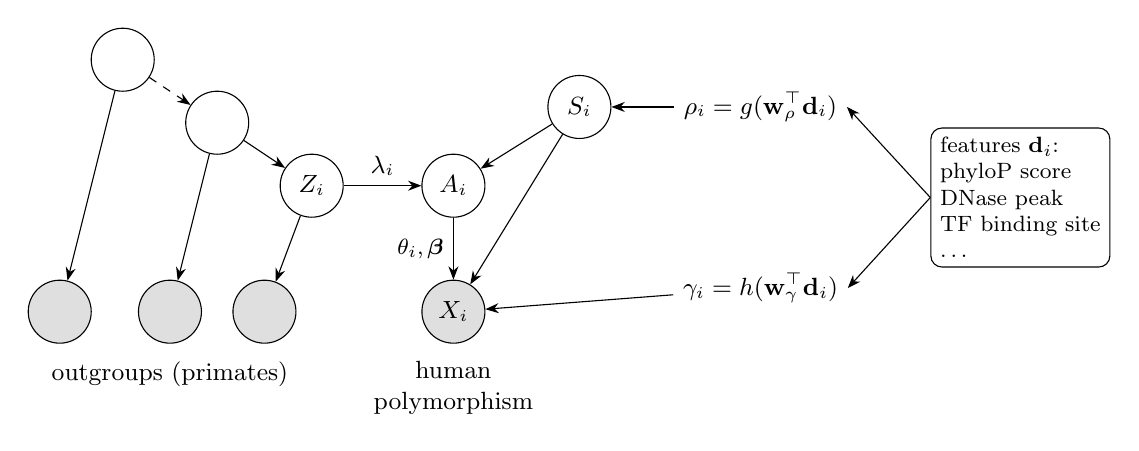
\begin{tikzpicture}[>=Stealth, every node/.style={font=\small},
      lat/.style={circle, draw, minimum size=8mm, inner sep=0pt},
      obs/.style={circle, draw, fill=gray!25, minimum size=8mm, inner sep=0pt},
      det/.style={diamond, draw, aspect=1, inner sep=1.5pt}]
    % outgroup tree
    \node[lat] (r) at (0,3.2) {};
    \node[lat] (n2) at (1.2,2.4) {};
    \node[lat] (Z) at (2.4,1.6) {$Z_i$};
    \node[obs] (o1) at (-0.8,0) {};
    \node[obs] (o2) at (0.6,0) {};
    \node[obs] (o3) at (1.8,0) {};
    \draw[->] (r) -- (o1); \draw[->, dashed] (r) -- (n2); \draw[->] (n2) -- (o2); \draw[->] (Z) -- (o3);
    \draw[->] (n2) -- (Z);
    \node[below=1mm of o2, align=center] {outgroups (primates)};
    \node[lat] (A) at (4.2,1.6) {$A_i$};
    \node[obs] (X) at (4.2,0) {$X_i$};
    \node[below=1mm of X, align=center] {human\\polymorphism};
    \draw[->] (Z) -- node[above] {$\lambda_i$} (A);
    \draw[->] (A) -- node[left, font=\footnotesize] {$\theta_i,\boldsymbol\beta$} (X);
    \node[lat] (Si) at (5.8,2.6) {$S_i$};
    \draw[->] (Si) -- (A); \draw[->] (Si) -- (X);
    \node (rho) at (8.1,2.6) {$\rho_i=g(\vw_\rho^\top\vd_i)$};
    \node (gam) at (8.1,0.3) {$\gamma_i=h(\vw_\gamma^\top\vd_i)$};
    \draw[->] (rho) -- (Si); \draw[->] (gam) -- (X);
    \node[draw, rounded corners, align=left, font=\footnotesize] (feat) at (11.4,1.45) {features $\vd_i$:\\phyloP score\\DNase peak\\TF binding site\\\dots};
    \draw[->] (feat.west) -- (rho.east); \draw[->] (feat.west) -- (gam.east);
  \end{tikzpicture}
  \caption{The LINSIGHT model for site $i$. Grey nodes are observed. Outgroup sequences inform the human-chimpanzee ancestral allele $Z_i$ and, with the neutral divergence rate $\lambda_i$, the human ancestral allele $A_i$. The observed human polymorphism data $X_i$ depend on the neutral polymorphism rate $\theta_i$, the neutral frequency spectrum $\boldsymbol\beta$ and the selection indicator $S_i$. The prior probability of selection $\rho_i$ and the relative rate of low-frequency polymorphism under selection $\gamma_i$ are functions of genomic features $\vd_i$. Redrawn after \citet{huang2017}.}
  \label{fig:linsight_model}
\end{figure}

Table~\ref{tab:linsight} lists the quantities in the model. For site $i$, the binary variable $S_i$ indicates whether the site is under selection, with prior probability $\rho_i$. To see how the likelihood works, assume the ancestral allele is known and classify the human data at site $i$ into five patterns: monomorphic with the ancestral allele ($\mathsf{M}$); monomorphic with a derived allele, that is, a substitution on the human lineage ($\mathsf{D}$); or polymorphic with the derived allele at low ($\mathsf{L}$), intermediate ($\mathsf{I}$) or high ($\mathsf{H}$) frequency. Under neutrality a polymorphism occurs with probability $\theta_i$ and its derived allele frequency falls into the three classes with probabilities $\boldsymbol\beta=(\beta_1,\beta_2,\beta_3)$, and a substitution occurs with probability $\lambda_i$. Under selection, substitutions and intermediate- or high-frequency polymorphisms are not allowed, and low-frequency polymorphisms occur at a rate reduced by the factor $\gamma_i$. This gives
\begin{center}
  \begin{tabular}{lcc}
    \toprule
    pattern $X_i$ & $P(X_i\mid S_i=0)$, neutral & $P(X_i\mid S_i=1)$, selected \\
    \midrule
    $\mathsf{M}$, monomorphic, ancestral & $(1-\theta_i)(1-\lambda_i)$ & $1-\gamma_i\theta_i$ \\
    $\mathsf{D}$, substitution & $(1-\theta_i)\lambda_i$ & $0$ \\
    $\mathsf{L}$, low-frequency derived & $\theta_i\beta_1$ & $\gamma_i\theta_i$ \\
    $\mathsf{I}$, intermediate-frequency derived & $\theta_i\beta_2$ & $0$ \\
    $\mathsf{H}$, high-frequency derived & $\theta_i\beta_3$ & $0$ \\
    \bottomrule
  \end{tabular}
\end{center}
Each column sums to one. INSIGHT also allows adaptive substitutions under selection; LINSIGHT drops this term because positive selection has a negligible effect at the genome-wide scale. The full model integrates over the uncertain ancestral allele with the outgroup phylogeny, and defines frequency classes by a threshold on the minor allele frequency, which complicates the expressions without changing their logic. Marginalizing over $S_i$, the likelihood of site $i$ is
\begin{equation}
  P(X_i) = \rho_i\,P(X_i\mid S_i=1) + (1-\rho_i)\,P(X_i\mid S_i=0) .
  \label{eq:linsight_lik}
\end{equation}

\begin{table}[!htbp]
  \centering
  \caption{Quantities in the LINSIGHT model, after \citet{huang2017}.}
  \label{tab:linsight}
  \begin{tabular}{lp{0.68\linewidth}}
    \toprule
    \multicolumn{2}{l}{\emph{Parameters inherited from INSIGHT}} \\
    $\rho_i$ & probability that site $i$ is under selection; the LINSIGHT score of site $i$ \\
    $\gamma_i$ & expected relative rate of low-frequency derived alleles at site $i$ given that it is under selection \\
    $\lambda_i$ & neutral substitution (divergence) rate at site $i$ \\
    $\theta_i$ & neutral polymorphism rate at site $i$ \\
    $\boldsymbol\beta=(\beta_1,\beta_2,\beta_3)$ & fractions of neutral polymorphisms with low-, intermediate- and high-frequency derived alleles \\
    \midrule
    \multicolumn{2}{l}{\emph{Variables inherited from INSIGHT}} \\
    $X_i$ & observed polymorphism data at site $i$: major allele, minor allele and minor allele frequency class \\
    $Z_i$ & human-chimpanzee ancestral allele at site $i$ \\
    $A_i$ & human ancestral allele at site $i$ \\
    $S_i$ & indicator of whether site $i$ is under selection \\
    \midrule
    \multicolumn{2}{l}{\emph{Components of the generalized linear model}} \\
    $\vd_i\in\R^m$ & genomic feature vector of site $i$ \\
    $\vw_\rho\in\R^m$ & weight vector for $\rho$ (free parameters) \\
    $\vw_\gamma\in\R^m$ & weight vector for $\gamma$ (free parameters) \\
    \bottomrule
  \end{tabular}
\end{table}

A single site carries almost no information: nearly all sites are monomorphic in a sample of a few dozen genomes, whether selected or not. INSIGHT obtained information by pooling many sites of the same type and estimating one $\rho$ for the group. LINSIGHT pools through features instead. Let $\vd_i\in\R^m$ be the feature vector of site $i$, including an intercept; the original model used $m=48$ features in three classes, conservation scores (phyloP, phastCons and others), predicted binding sites (transcription factor and microRNA binding sites, splice sites) and regional annotations (ChIP-seq, DNase-seq and histone modification peaks, enhancer annotations, distance to the nearest transcription start site). The two selection parameters are
\begin{equation}
  \rho_i = g(\vw_\rho^\top\vd_i), \qquad \gamma_i = h(\vw_\gamma^\top\vd_i),
\end{equation}
with weight vectors $\vw_\rho,\vw_\gamma\in\R^m$. The link $h$ is the logistic function. For $g$, LINSIGHT uses the asymmetric Gompertz function $g(x)=\exp(-3e^{-x})$, which, unlike the logistic, keeps the gradient from vanishing when $\rho_i$ is close to zero, as it is at most sites. The neutral parameters $\lambda_i$, $\theta_i$ and $\boldsymbol\beta$ are estimated beforehand from the flanking neutral regions and held fixed. The weights maximize the log likelihood $\sum_i\log P(X_i)$ over all noncoding sites in the genome, billions of terms, which is done by stochastic gradient ascent on minibatches of sites (Chapter 2). The model is a generalized linear model whose ``response'' $X_i$ is linked to the linear predictor through the mixture~\eqref{eq:linsight_lik} rather than through a standard exponential family.

The LINSIGHT score of a site is $\rho_i$, the \emph{prior} probability of selection given its features, not the posterior $P(S_i=1\mid X_i)$. This is deliberate: the score of a site should not depend on whether a polymorphism happens to have been observed there in 54 genomes, and the prior is defined for every site, including those where a patient carries a variant never seen before. Because $\rho_i$ is a probability that a mutation at site $i$ is selected against, it is also called the \emph{fitness consequence} of the site. Figure~\ref{fig:linsight_fitness}a shows that it behaves as expected across annotation classes: low for intergenic and intronic sites, higher for UTRs, promoters and binding sites, and highest at splice sites.

\begin{figure}[!htbp]
  \centering
  \includegraphics[width=0.75\linewidth]{slides/linsight_fitness.png}
  \caption{(a) Distribution of LINSIGHT scores (fitness consequence, log scale) of noncoding sites in different annotation classes. TFBS, transcription factor binding site. (b) LINSIGHT and other scores around a noncoding disease variant from the Human Gene Mutation Database. LINSIGHT is elevated across the DNase hypersensitive region containing the variant, whereas the conservation scores (phastCons, phyloP, GERP++) give little signal at the variant itself. Reproduced from \citet{huang2017}.}
  \label{fig:linsight_fitness}
\end{figure}

\subsection{Evaluating pathogenicity scores}

To evaluate a predictor we need variants of known effect. \citet{huang2017} used noncoding variants from the Human Gene Mutation Database (HGMD), which catalogues variants reported to cause inherited disease, and from ClinVar, as positives, and common SNPs (MAF $>1\%$) as negatives. The ROC curves (Chapter 1) in Figure~\ref{fig:linsight_roc} show LINSIGHT ahead of the alternatives, with phyloP, which uses conservation alone, the weakest. Two caveats apply to this kind of benchmark. Common variants are an easy negative set, since a variant that has risen to high frequency is unlikely to be strongly deleterious, so the task differs from the clinical one of distinguishing a pathogenic rare variant from a benign rare variant. The authors therefore also used negatives matched to the positives by distance to the transcription start site, or drawn from within 1 kb of each disease variant. And the positives are biased toward regions people have looked at, such as promoters of known disease genes, so methods that learn ``near a known disease gene'' are rewarded.

\begin{figure}[!htbp]
  \centering
  \includegraphics[width=0.5\linewidth]{slides/linsight_hgmd_roc.png}
  \caption{ROC curves (true positive rate against false positive rate) for distinguishing noncoding disease variants from HGMD from common SNPs not matched to the disease variants by location. phyloP, conservation across species; CADD, a classifier of observed against simulated variants; FunSeq2 and DeepSEA, see text; Eigen, an unsupervised combination of annotations. Reproduced from \citet{huang2017}.}
  \label{fig:linsight_roc}
\end{figure}

%======================================================================
\section{Variance component tests: SKAT and SKAT-O}
\label{sec:skat}
%======================================================================

Burden tests assume that all qualifying variants act in the same direction. This is reasonable for loss-of-function variants in a gene where losing one copy is harmful, but not in general. Some missense variants increase protein activity and others decrease it; in a regulatory region some variants increase expression and others decrease it; and most variants in a region may be neutral. The sequence kernel association test (SKAT)~\citep{wu2011} drops the assumption by treating the per-variant effects as random with mean zero, and SKAT-O~\citep{lee2012} interpolates between SKAT and the burden test.

\subsection{The model}

Let $\vg_i\in\{0,1,2\}^M$ be the genotypes of individual $i$ at the $M$ variants, so that $\vg_i^\top$ is row $i$ of $\mG$. The per-variant model is
\begin{equation}
  h(\mu_i) = \vx_i^\top\valpha + \vg_i^\top\vb, \qquad \vb\in\R^M,
\end{equation}
with $\vb$ random and
\begin{equation}
  \E[\beta_j]=0, \qquad \Var(\beta_j)=w_j^2\tau, \qquad \Cov(\beta_{j_1},\beta_{j_2})=\rho\,w_{j_1}w_{j_2}\tau \quad (j_1\neq j_2),
  \label{eq:skat_prior}
\end{equation}
where $\tau\geq 0$ is a variance component, $w_j$ is the weight of variant $j$ and $\rho\in[0,1]$ is the correlation between effects. In matrix form, $\Cov(\vb)=\tau\mW\mR_\rho\mW$, with $\mW=\operatorname{diag}(\vw)$ and $\mR_\rho=(1-\rho)\mI_M+\rho\ind\ind^\top$, where $\ind$ is the vector of $M$ ones. Two cases are of interest. With $\rho=0$ the effects are independent, with random signs and magnitudes that scale with $w_j$; this is SKAT, also called a \emph{dispersion} test, because it detects effects that spread the trait in either direction. With $\rho=1$ the effects are perfectly correlated, so $\vb=\vw\beta_0$ for a single random $\beta_0$ with variance $\tau$, which is the burden model~\eqref{eq:burden_glm}. The null hypothesis $\vb=\mathbf{0}$ becomes $H_0:\tau=0$, a test of one parameter however many variants the region contains.

\subsection{Deriving the score statistic}

For a quantitative trait with Gaussian noise, take $\vb$ to be Gaussian as well. Then $\vb$ can be integrated out, as for ridge regression in Chapter 1, and
\begin{equation}
  \vy\sim\Normal\left(\mX\valpha,\ \mSigma(\tau)\right), \qquad \mSigma(\tau) = \sigma^2\mI_N + \tau\mK, \qquad \mK = \mG\mW\mR_\rho\mW\mG^\top ,
\end{equation}
where $\mK\in\R^{N\times N}$ is a kernel matrix: $K_{ii'}$ measures the weighted genetic similarity of individuals $i$ and $i'$ in the region. Let $\vr=\vy-\mX\valpha$. The log likelihood is $\ell(\tau)=-\frac{1}{2}\log|\mSigma(\tau)|-\frac{1}{2}\vr^\top\mSigma(\tau)^{-1}\vr+\text{const}$. Using $\partial\log|\mSigma|/\partial\tau=\tr(\mSigma^{-1}\partial\mSigma/\partial\tau)$ and $\partial\mSigma^{-1}/\partial\tau=-\mSigma^{-1}(\partial\mSigma/\partial\tau)\mSigma^{-1}$, with $\partial\mSigma/\partial\tau=\mK$,
\begin{equation}
  \frac{\partial\ell}{\partial\tau} = -\frac{1}{2}\tr\left(\mSigma^{-1}\mK\right) + \frac{1}{2}\vr^\top\mSigma^{-1}\mK\mSigma^{-1}\vr .
\end{equation}
At $\tau=0$, $\mSigma=\sigma^2\mI$ and
\begin{equation}
  \left.\frac{\partial\ell}{\partial\tau}\right|_{\tau=0} = \frac{1}{2\sigma^4}\vr^\top\mK\vr - \frac{1}{2\sigma^2}\tr(\mK) .
\end{equation}
The trace term does not depend on the data, so the test can be based on the quadratic form in the residuals $\hat\vr=\vy-\mX\hat\valpha$ from the null model. Substituting $\mK$ and the score vector $\vS=\mG^\top\hat\vr$ from~\eqref{eq:score},
\begin{equation}
  Q_\rho = \hat\vr^\top\mK\hat\vr = \vS^\top\mW\mR_\rho\mW\vS
  = (1-\rho)\underbrace{\sum_{j=1}^M w_j^2S_j^2}_{Q_{\text{SKAT}}} + \rho\underbrace{\Big(\sum_{j=1}^M w_jS_j\Big)^2}_{Q_{\text{burden}}} .
  \label{eq:skat_q}
\end{equation}
The SKAT statistic is a weighted sum of the squared single-variant score statistics, and the burden statistic is the square of their weighted sum. The difference explains when each works. Under the alternative, $\E[S_j]$ has the sign of $\beta_j$ (for variants in weak linkage disequilibrium). Squaring before summing makes $Q_{\text{SKAT}}$ insensitive to the signs, while in $Q_{\text{burden}}$ variants with opposite effects cancel. Conversely, when all effects share a sign, $Q_{\text{burden}}$ adds their signals coherently while $Q_{\text{SKAT}}$ also accumulates noise from the squared scores of neutral variants. For binary traits the same argument applied to a logistic mixed model gives a score statistic of the same form~\eqref{eq:skat_q}, with residuals $y_i-\hat\mu_i$ from the null logistic regression~\citep{wu2011}.

The SKAT framework allows any positive semi-definite kernel in place of $\mG\mW\mW\mG^\top$, for example kernels based on the number of alleles two people share identical by state, which can capture interactions between variants~\citep{wu2011}. The weighted linear kernel is the one used in practice.

\subsection{The null distribution}

Under $H_0$, $\vS\sim\Normal(\mathbf{0},\sigma^2\boldsymbol{\Omega})$ with $\boldsymbol{\Omega}=\mG^\top\mP_0\mG\in\R^{M\times M}$, as shown in Section~\ref{sec:burden}. Write $\vS=\sigma\boldsymbol{\Omega}^{1/2}\vz$ with $\vz\sim\Normal(\mathbf{0},\mI_M)$ and let $\mathbf{A}_\rho=\mW\mR_\rho\mW$. Then
\begin{equation}
  \frac{Q_\rho}{\sigma^2} = \vz^\top\boldsymbol{\Omega}^{1/2}\mathbf{A}_\rho\boldsymbol{\Omega}^{1/2}\vz = \sum_{k=1}^M \lambda_k u_k^2, \qquad u_k\overset{\text{iid}}{\sim}\Normal(0,1),
\end{equation}
where $\lambda_1,\dots,\lambda_M\geq 0$ are the eigenvalues of $\boldsymbol{\Omega}^{1/2}\mathbf{A}_\rho\boldsymbol{\Omega}^{1/2}$ and the second equality follows by rotating $\vz$ into its eigenbasis. The null distribution of $Q_\rho/\sigma^2$ is therefore a weighted sum of independent $\chi^2_1$ variables. Its tail probability has no closed form but can be computed by numerically inverting the characteristic function~\citep{davies1980} or approximated by matching moments to a scaled $\chi^2$~\citep{liu2009}. In practice $\sigma^2$ is replaced by its estimate under the null. For burden ($\rho=1$) the matrix $\mathbf{A}_1=\vw\vw^\top$ has rank one, a single eigenvalue $\lambda_1=\vw^\top\boldsymbol{\Omega}\vw$ is non-zero, and we recover the $\chi^2_1$ test of Section~\ref{sec:burden}.

\subsection{Variant weights}

The default SKAT weights are the $\BetaD(1,25)$ density evaluated at the MAF, $w_j=25(1-f_j)^{24}$ (Figure~\ref{fig:maf_weights}). The weight is nearly constant for $f_j$ below about 0.005 and falls to almost zero by $f_j=0.1$, so rare variants dominate the statistic, which encodes the expectation from Figure~\ref{fig:effect_freq} that rarer variants have larger effects. Under~\eqref{eq:skat_prior} the expected contribution of variant $j$ to the trait variance is $2f_j(1-f_j)w_j^2\tau$, so the choice of weights is a prior on how variance explained is spread across the frequency spectrum. The weights are also the natural place to put functional information, a point we return to in Section~\ref{sec:fst}.

\begin{figure}[!htbp]
  \centering
  \includegraphics[width=0.8\linewidth]{maf_weights.pdf}
  \caption{Variant weights as a function of MAF, each scaled to a maximum of one: the $\BetaD(1,25)$ density used by default in SKAT, the Madsen-Browning weight $1/\sqrt{f(1-f)}$, and equal weights.}
  \label{fig:maf_weights}
\end{figure}

\subsection{SKAT-O}

We rarely know in advance whether a gene's variants act in one direction. SKAT-O~\citep{lee2012} computes $Q_\rho$ over a grid $0=\rho_1<\rho_2<\dots<\rho_B=1$, for example $\rho\in\{0,0.1^2,0.2^2,0.3^2,0.4^2,0.5^2,1\}$, and uses the smallest p-value,
\begin{equation}
  T = \min_{b=1,\dots,B} p_{\rho_b},
\end{equation}
where $p_{\rho_b}$ is the p-value of $Q_{\rho_b}$. $T$ is not itself a p-value, because taking the minimum over several tests makes small values more likely. Its null distribution follows from the joint distribution of the $Q_\rho$, which are all quadratic forms in the same $\vS$. Because $Q_\rho$ is linear in $\rho$, it is a combination of $Q_{\text{SKAT}}$ and $Q_{\text{burden}}$, and \citet{lee2012} decompose it into a $\chi^2_1$ part and an approximately independent remainder, which reduces the p-value of $T$ to a one-dimensional numerical integral. They also give a small-sample correction for binary traits, where the asymptotic null distribution can be poor.

Why not estimate $\rho$, for example by maximum likelihood, and plug it in? Under $H_0$, $\tau=0$ and $\rho$ has no effect on the likelihood: it is not identifiable. A parameter that exists only under the alternative breaks the usual asymptotic theory for likelihood ratio and score tests, so the plug-in statistic has no standard null distribution. Taking the minimum p-value over a grid and computing the exact null distribution of the minimum sidesteps the problem. The price is a modest loss of power relative to knowing the best $\rho$ in advance.

\subsection{Comparing the tests}

Figure~\ref{fig:skat_power} compares the three tests in a simulated region of 39 rare variants. When most variants are causal and all increase the trait, the burden test is the most powerful. When few variants are causal, or when effects have mixed signs, SKAT is much more powerful, and with mixed signs the burden test has almost no power at all. SKAT-O is close to the better of the two in every setting. It is never the best by much, but it is never far from the best, which is why it is a common default.

\begin{figure}[!htbp]
  \centering
  \includegraphics[width=0.9\linewidth]{skat_power.pdf}
  \caption{Power of burden, SKAT and SKAT-O tests (with $\BetaD(1,25)$ weights) in a simulated region of $M=39$ independent variants with MAF between 0.0005 and 0.02, for a quantitative trait in $N=2000$ individuals. Each variant is causal with the probability on the horizontal axis and has effect $|\beta_j|=a|\log_{10}f_j|$, with the sign either always positive (left) or random (right). The scale $a$ is smaller for larger causal fractions, so power should be compared between tests within a group of bars, not across groups. Null distributions were computed by simulating $2\times10^5$ score vectors for the fixed genotype matrix; 1000 replicates per setting.}
  \label{fig:skat_power}
\end{figure}

%======================================================================
\section{Using functional annotations in the test}
\label{sec:fst}
%======================================================================

A pathogenicity score such as LINSIGHT, CADD or Eigen gives, for each variant, an estimate of how likely it is to be functional. There are two simple ways to use it in a set-based test: filter variants on a threshold, as in a burden analysis, or multiply the MAF weights by the score, $w_j\to w_jZ_j$, where $Z_j\geq 0$ is the score of variant $j$. Both help if the score predicts which variants affect the trait and hurt if it does not. For noncoding variants, where scores are weak and a score built for one purpose (say, conservation) may not predict effects on a particular trait, this matters. \citet{he2017} proposed tests that use several annotations at once and lose little power when an annotation is uninformative. We call this the functional score test (FST).

\subsection{The model}

Let $q$ be the number of annotations and $Z_{jk}$ the $k$-th functional score of variant $j$, $k=1,\dots,q$. The effect of variant $j$ is decomposed as
\begin{equation}
  \beta_j = \gamma_{j0} + \sum_{k=1}^q Z_{jk}\gamma_{jk} ,
\end{equation}
where each $\gamma_{jk}$ is random with mean zero, $\Var(\gamma_{jk})=w_j^2\tau_k$ and $\Cov(\gamma_{j_1k},\gamma_{j_2k})=\rho\,w_{j_1}w_{j_2}\tau_k$, and the $\gamma_{j0},\dots,\gamma_{jq}$ are independent for each $j$. The variance component $\tau_k\geq 0$ measures how much of the genetic effect in the region tracks annotation $k$, and $\tau_0$ the part that tracks no annotation. Then
\begin{align}
  \Var(\beta_j) &= w_j^2\Big(\tau_0+\sum_{k=1}^q Z_{jk}^2\tau_k\Big), \\
  \Cov(\beta_{j_1},\beta_{j_2}) &= \rho\,w_{j_1}w_{j_2}\Big(\tau_0+\sum_{k=1}^q Z_{j_1k}Z_{j_2k}\tau_k\Big).
\end{align}
Setting $Z_{j0}=1$ and $\mD_k=\operatorname{diag}(w_1Z_{1k},\dots,w_MZ_{Mk})$, the covariance of $\vb$ is a sum of SKAT-O covariances, one per annotation,
\begin{equation}
  \Cov(\vb) = \sum_{k=0}^q \tau_k\,\mD_k\mR_\rho\mD_k ,
\end{equation}
and the null hypothesis of no association is $H_0:\tau_0=\tau_1=\dots=\tau_q=0$.

\subsection{The test}

Repeating the derivation of Section~\ref{sec:skat} for each $\tau_k$ in turn gives one score statistic per annotation,
\begin{equation}
  Q_{\rho,k} = \vS^\top\mD_k\mR_\rho\mD_k\vS = (1-\rho)\sum_{j=1}^M w_j^2Z_{jk}^2S_j^2 + \rho\Big(\sum_{j=1}^M w_jZ_{jk}S_j\Big)^2 ,
\end{equation}
which is the SKAT-O statistic with weights $w_jZ_{jk}$. $Q_{\rho,0}$ is the original test with MAF weights only. \citet{he2017} combine these statistics by their minimum p-value, $T=\min_{k,\rho}p_{\rho,k}$, over $k=0,\dots,q$ and, in practice, $\rho\in\{0,1\}$, so that the combined test takes the best of the dispersion and burden tests for each annotation. The null distribution of $T$ is obtained from the null distribution of $\vS$ alone. Score vectors are drawn from $\Normal(\mathbf{0},\hat\sigma^2\boldsymbol{\Omega})$, each $p_{\rho,k}$ is computed by moment matching, and the vector of normal scores $\boldsymbol\delta$ with elements $\Phi^{-1}(p_{\rho,k})$ is approximated as multivariate normal with the correlation matrix estimated from the draws. The p-value of an observed $T=t$ is then $1-P(\delta_{\rho,k}>\Phi^{-1}(t)\text{ for all }k,\rho)$, a multivariate normal probability. Only $\vS$ and $\boldsymbol{\Omega}$ are needed, so the test works with summary statistics and, by adding them across studies, in meta-analysis.

The construction has a simple logic. The unified test always contains the original test, $k=0$, so when the annotations are uninformative it loses only what the multiple-testing correction across the $2(q+1)$ statistics costs. When an annotation is informative, the corresponding reweighted statistic carries the signal.

\subsection{Power}

\citet{he2017} simulated regions in which 10\% of variants were causal and annotation $k$ predicted the causal variants with probability $P_k$. They compared the original tests with $\BetaD(1,25)$ weights (O), tests with weights multiplied by the first score (W1), and unified tests with the first score (U1) or the first two scores (U1+2). When neither score was informative ($P_1=P_2=0$), W1 lost a large fraction of the power of O while U1 and U1+2 lost none, and could even gain slightly. When the first score was informative, W1, U1 and U1+2 all improved on O. When only the second score was informative, U1+2 was the most powerful and W1 the least. The pattern held for dispersion, burden and combined tests.

Figure~\ref{fig:fst_power} reproduces the logic in a small simulation of our own, using a region simulated as in Figure~\ref{fig:skat_power} and a single annotation. With an uninformative score, reweighting (W) costs most of the power, while the unified test (U) stays close to the original (O). With an informative score, reweighting helps the burden test a great deal, because it removes the neutral variants that dilute the burden, and the unified test captures most of the gain. SKAT gains less from the annotation, since squaring the scores already lets the variants with large $S_j$ dominate.

\begin{figure}[!htbp]
  \centering
  \includegraphics[width=0.9\linewidth]{fst_power.pdf}
  \caption{Power of SKAT and burden tests with $\BetaD(1,25)$ weights (O), weights multiplied by a functional score (W), and the unified minimum p-value test over both weightings (U). In a region simulated as in Figure~\ref{fig:skat_power}, 20\% of variants are causal with positive effects $\beta_j=0.28|\log_{10}f_j|$. The score is $\chi^2_1$ for non-causal variants; for each causal variant it is non-central $\chi^2_1$ (non-centrality 4) with probability $P$ and $\chi^2_1$ otherwise. 50 draws of the causal set and scores, 20 trait replicates each, $\alpha=10^{-3}$. Within a panel the tests are applied to the same simulated traits.}
  \label{fig:fst_power}
\end{figure}

%======================================================================
\section{Case study: noncoding de novo mutations in autism}
\label{sec:autism}
%======================================================================

Autism spectrum disorder (ASD) has a substantial contribution from de novo mutations. Exome sequencing of families found that children with ASD carry more de novo protein-truncating mutations than their unaffected siblings~\citep{iossifov2014}, and burden tests of such mutations have identified many ASD genes. In Chapter 10 we saw that de novo mutations predicted by SpliceAI to disrupt splicing are also enriched in ASD and intellectual disability. Most de novo mutations, about 70 per genome, fall outside coding sequence, and whether noncoding de novo mutations contribute was an open question. Noncoding mutations cannot be tested one at a time, and there is no simple equivalent of ``protein-truncating'' to define which ones to aggregate. \citet{zhou2019} used deep learning sequence models to supply that definition.

\subsection{Data and design}

The data were whole genomes from 1,790 \emph{simplex} families from the Simons Simplex Collection, 7,097 genomes in total. A simplex family has exactly one affected child, the proband, together with unaffected parents and, in most families, an unaffected sibling (Figure~\ref{fig:asd_pipeline}). Simplex families are enriched for de novo causes, because an inherited cause of large effect would often have affected other family members. The unaffected siblings are a natural control group. They have the same parents, so their expected de novo mutation rate is similar, and their genomes were sequenced and processed in the same way as the probands', so technical artefacts in mutation calling affect both groups alike. The comparison is therefore between the de novo mutations of probands and those of siblings, and the question is whether the probands' mutations are more damaging.

\subsection{Scoring mutations}

Each de novo mutation was scored with two DeepSEA-style convolutional networks (Chapter 2), which take 1,000 bp of sequence centred on the variant and predict the probability of each of many chromatin or RNA-binding features. The transcriptional regulation model predicts 2,002 features (DNase hypersensitivity, transcription factor binding and histone marks) and was trained on ENCODE and Roadmap Epigenomics profiles. The post-transcriptional model predicts 232 features, mostly RNA-binding protein (RBP) binding sites measured by CLIP-seq, which captures the sites on RNA bound by a given protein. For each mutation and feature $\ell$, the variant effect is the absolute difference between the predictions for the two alleles, $|p_\ell(\text{alt})-p_\ell(\text{ref})|$.

These thousands of predicted effects must be reduced to one number per mutation, the probability that it is harmful. \citet{zhou2019} trained a regularized logistic regression (Chapter 1) with the standardized predicted effects as features, separately for transcriptional and post-transcriptional effects. Positive examples were 4,401 noncoding regulatory mutations reported in HGMD to cause disease. Negative examples were 999,668 \emph{singleton} variants observed in healthy individuals in the 1000 Genomes Project. Singletons are a better negative set than common variants because they are rare, like de novo mutations, and so have similar sequence context and mutational processes; they are mostly benign, but selection has had little time to remove the damaging ones, so the negative set is somewhat contaminated. Classes were weighted inversely to their size to counter the imbalance. The predicted probabilities were standardized across all proband and sibling mutations to give a \emph{disease impact score} (DIS) for each mutation. The classifier never sees autism data: it learns what Mendelian disease mutations look like through the eyes of the sequence models, and is then applied to a different disease.

\begin{figure}[!htbp]
  \centering
  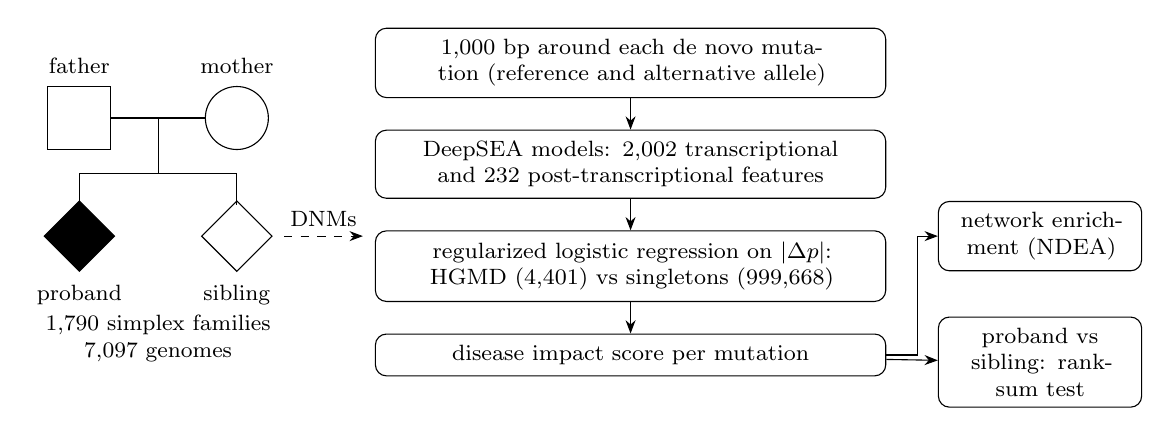
\begin{tikzpicture}[>=Stealth, every node/.style={font=\small},
      box/.style={draw, rounded corners, align=center, inner sep=4pt}]
    % pedigree
    \node[draw, minimum size=8mm] (fa) at (0,2.2) {};
    \node[draw, circle, minimum size=8mm] (mo) at (2.0,2.2) {};
    \node[above=1pt of fa, font=\footnotesize] {father};
    \node[above=1pt of mo, font=\footnotesize] {mother};
    \draw (fa.east) -- (mo.west);
    \draw (1.0,2.2) -- (1.0,1.5) -- (0,1.5) -- (0,1.1);
    \draw (1.0,1.5) -- (2.0,1.5) -- (2.0,1.1);
    \node[draw, diamond, fill=black, minimum size=9mm, inner sep=0pt] (pr) at (0,0.7) {};
    \node[draw, diamond, minimum size=9mm, inner sep=0pt] (sb) at (2.0,0.7) {};
    \node[below=1pt of pr, font=\footnotesize] {proband};
    \node[below=1pt of sb, font=\footnotesize] {sibling};
    \node[align=center, font=\footnotesize] at (1.0,-0.6) {1,790 simplex families\\7,097 genomes};
    % pipeline
    \begin{scope}[box/.append style={text width=6.2cm, font=\footnotesize}]
    \node[box] (seq) at (7.0,2.9) {1,000 bp around each de novo mutation (reference and alternative allele)};
    \node[box, below=4mm of seq] (cnn) {DeepSEA models: 2,002 transcriptional and 232 post-transcriptional features};
    \node[box, below=4mm of cnn] (lr) {regularized logistic regression on $|\Delta p|$: HGMD (4,401) vs singletons (999,668)};
    \node[box, below=4mm of lr] (dis) {disease impact score per mutation};
    \end{scope}
    \node[box, text width=2.3cm, font=\footnotesize] (cmp) at (12.2,-0.9) {proband vs sibling: rank-sum test};
    \node[box, text width=2.3cm, font=\footnotesize] (nd) at (12.2,0.7) {network enrichment (NDEA)};
    \draw[->] (seq) -- (cnn); \draw[->] (cnn) -- (lr); \draw[->] (lr) -- (dis);
    \draw[->] (dis) -- (cmp); \draw[->] (dis.east) -- ++(0.4,0) |- (nd.west);
    \draw[->, dashed] (2.6,0.7) -- (3.6,0.7) node[midway, above, font=\footnotesize] {DNMs};
  \end{tikzpicture}
  \caption{Design of the autism noncoding mutation study. Each simplex family has one affected child (proband, filled) and an unaffected sibling. De novo mutations (DNMs) are scored by sequence models, the predicted effects are combined into a disease impact score by a classifier trained on known disease mutations, and the scores of proband and sibling mutations are compared. After \citet{zhou2019}.}
  \label{fig:asd_pipeline}
\end{figure}

\subsection{Comparing probands and siblings}

The scores of proband and sibling mutations were compared with a one-sided Wilcoxon rank-sum (Mann-Whitney) test. Let $d^P_1,\dots,d^P_{n_P}$ be the DIS values of proband mutations and $d^S_1,\dots,d^S_{n_S}$ those of sibling mutations. Rank all $n_P+n_S$ values together, let $R_P$ be the sum of the ranks of the proband mutations, and define $U=R_P-n_P(n_P+1)/2$, the number of (proband, sibling) pairs in which the proband mutation has the higher score. Under the null hypothesis that the two groups have the same distribution, and with no ties,
\begin{equation}
  \E[U]=\frac{n_Pn_S}{2}, \qquad \Var(U)=\frac{n_Pn_S(n_P+n_S+1)}{12},
\end{equation}
and $(U-\E[U])/\sqrt{\Var(U)}$ is approximately standard normal for large samples. The test uses only ranks, so it is robust to the heavy tail of the score distribution, in which a few mutations have very high predicted impact. The quantity $U/(n_Pn_S)$ is the probability that a random proband mutation scores higher than a random sibling mutation, the same quantity as the AUROC of Chapter 1.

Proband mutations had significantly higher disease impact scores than sibling mutations, for both transcriptional and post-transcriptional effects (Figure~\ref{fig:asd_dis}). The difference was larger for mutations near genes, and larger again near genes that are intolerant of loss-of-function variation in the population. The effect is small on average, as expected if only a minority of probands carry a causal noncoding mutation.

\begin{figure}[!htbp]
  \centering
  \includegraphics[width=0.7\linewidth]{slides/asd_disease_impact.png}
  \caption{Mean disease impact score of de novo mutations in probands (red) and unaffected siblings (grey), for predicted transcriptional (DNA) and post-transcriptional (RNA) effects. Scores are normalized by subtracting the sibling mean, so siblings are at zero; bars show 95\% confidence intervals. Mutations are shown for all variants, variants assigned to any gene, and variants assigned to genes intolerant of loss of function, with the significance of each comparison above; all comparisons have false discovery rate below 0.05. Reproduced from \citet{zhou2019}.}
  \label{fig:asd_dis}
\end{figure}

%======================================================================
\section{Network differential enrichment analysis}
\label{sec:ndea}
%======================================================================

Even with a good score, de novo mutations are too sparse to implicate individual genes: most genes receive no mutation in either group, and few receive more than one. \citet{zhou2019} therefore borrowed strength across genes using a gene network. The network was the brain-specific functional network of \citet{greene2015}, one of a set of tissue-specific networks built by Bayesian integration of thousands of genome-scale data sets (expression, protein interactions, and others) against tissue-specific gold standards. Unlike the co-expression and partial-correlation networks of Chapter 9, its edges are not estimated from one data type: the weight $A_{uv}\in[0,1]$ is the posterior probability that genes $u$ and $v$ act together in brain.

Network differential enrichment analysis (NDEA) asks, for each gene $u$, whether the mutations in genes functionally connected to $u$ have higher scores in probands than in siblings. Let $\mathcal{P}$ and $\mathcal{S}$ be the sets of proband and sibling mutations, $d_m$ the disease impact score of mutation $m$, and $v(m)$ the gene to which it is assigned (the nearest gene within a distance threshold). Each mutation receives a weight for gene $u$,
\begin{equation}
  a_{um} = \frac{A_{u,v(m)}}{n_{v(m)}} ,
\end{equation}
where $n_{v}$ is the number of mutations in the same group (proband or sibling) assigned to gene $v$, so that a gene with many mutations does not dominate. The weighted mean scores of the two groups are
\begin{equation}
  \mu_{\mathcal{P}}(u) = \frac{\sum_{m\in\mathcal{P}}a_{um}d_m}{\sum_{m\in\mathcal{P}}a_{um}}, \qquad
  \mu_{\mathcal{S}}(u) = \frac{\sum_{m\in\mathcal{S}}a_{um}d_m}{\sum_{m\in\mathcal{S}}a_{um}} ,
\end{equation}
and they are compared with a weighted version of Welch's $t$ statistic,
\begin{equation}
  t_u = \frac{\mu_{\mathcal{P}}(u)-\mu_{\mathcal{S}}(u)}{\sqrt{V_{\mathcal{P}}(u)/N_{\mathcal{P}}(u)+V_{\mathcal{S}}(u)/N_{\mathcal{S}}(u)}} .
  \label{eq:ndea}
\end{equation}
Here, for group $\mathcal{G}\in\{\mathcal{P},\mathcal{S}\}$, dropping the dependence on $u$,
\begin{equation}
  V_{\mathcal{G}} = \frac{\sum_{m\in\mathcal{G}}a_{m}(d_m-\mu_{\mathcal{G}})^2}{\sum_{m\in\mathcal{G}}a_m-\sum_{m\in\mathcal{G}}a_m^2\big/\sum_{m\in\mathcal{G}}a_m}, \qquad
  N_{\mathcal{G}} = \frac{\left(\sum_{m\in\mathcal{G}}a_m\right)^2}{\sum_{m\in\mathcal{G}}a_m^2} .
\end{equation}
Both quantities generalize their unweighted counterparts. Suppose the $d_m$ in a group are independent with mean $\mu$ and variance $v$, and the weights are fixed. Writing $A_1=\sum_m a_m$ and $A_2=\sum_m a_m^2$, the weighted mean $\hat\mu=\sum_m a_md_m/A_1$ has variance
\begin{equation}
  \Var(\hat\mu) = \frac{\sum_m a_m^2 v}{A_1^2} = \frac{v}{N}, \qquad N=\frac{A_1^2}{A_2},
\end{equation}
so $N$ is the \emph{effective sample size}: the number of equally weighted observations that would give the same variance. It equals the number of mutations when the weights are equal, and is smaller when a few mutations carry most of the weight. For the variance, $\sum_ma_m(d_m-\hat\mu)^2=\sum_ma_md_m^2-A_1\hat\mu^2$, with $\E[\sum_ma_md_m^2]=A_1(v+\mu^2)$ and $\E[\hat\mu^2]=\mu^2+vA_2/A_1^2$, so
\begin{equation}
  \E\Big[\sum_ma_m(d_m-\hat\mu)^2\Big] = A_1(v+\mu^2) - A_1\mu^2 - v\frac{A_2}{A_1} = v\left(A_1-\frac{A_2}{A_1}\right),
\end{equation}
and $V$ is an unbiased estimate of $v$. With equal weights $a_m=1$ in a group of $n$ mutations, $A_1=n$, $A_2=n$, $N=n$ and $V=\sum_m(d_m-\hat\mu)^2/(n-1)$, the usual sample variance, so~\eqref{eq:ndea} reduces to Welch's $t$. The statistic is compared with a $t$ distribution whose degrees of freedom follow from the Welch-Satterthwaite approximation with $N_{\mathcal{P}}$ and $N_{\mathcal{S}}$ in place of the group sizes.

A gene can score highly without carrying a single mutation, if its network neighbours carry high-impact proband mutations (Figure~\ref{fig:ndea}). The same test applies to a gene set, such as a Gene Ontology (GO) term, by treating the set as one node whose edge weight to gene $v$ is the average of $A_{u v}$ over the genes $u$ in the set. Among the terms enriched at false discovery rate below 0.05 were many neuronal functions: regulation of synapse assembly, axon guidance, dendrite development, the synaptic vesicle cycle, postsynaptic density and neuron migration. Clustering the top-ranked genes on the network gave groups related to synaptic function and to chromatin regulation. Both themes had already emerged from coding de novo mutations in ASD: genes for synaptic function, which are specific to neurons, and genes for transcriptional and chromatin regulation, which act in every cell type yet seem to matter most for neurodevelopment. The noncoding mutations point to the same biology.

\begin{figure}[!htbp]
  \centering
  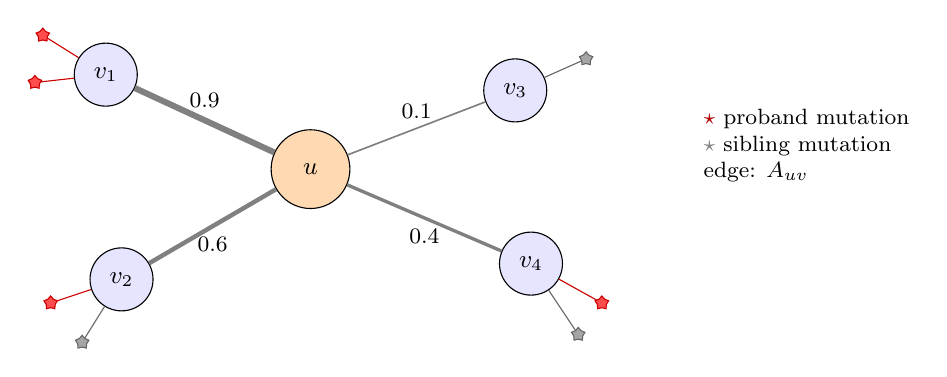
\begin{tikzpicture}[>=Stealth, every node/.style={font=\small},
      gene/.style={circle, draw, minimum size=8mm, inner sep=0pt, fill=blue!10}]
    \node[gene, fill=orange!30, minimum size=10mm] (u) at (0,0) {$u$};
    \node[gene] (v1) at (-2.6,1.2) {$v_1$};
    \node[gene] (v2) at (-2.4,-1.4) {$v_2$};
    \node[gene] (v3) at (2.6,1.0) {$v_3$};
    \node[gene] (v4) at (2.8,-1.2) {$v_4$};
    \draw[line width=2.2pt, gray] (u) -- node[above, black, font=\footnotesize] {0.9} (v1);
    \draw[line width=1.6pt, gray] (u) -- node[below, black, font=\footnotesize] {0.6} (v2);
    \draw[line width=0.6pt, gray] (u) -- node[above, black, font=\footnotesize] {0.1} (v3);
    \draw[line width=1.2pt, gray] (u) -- node[below, black, font=\footnotesize] {0.4} (v4);
    \foreach \n/\c/\dx/\dy in {v1/red/-0.8/0.5, v1/red/-0.9/-0.1, v2/red/-0.9/-0.3, v2/gray/-0.5/-0.8, v3/gray/0.9/0.4, v4/red/0.9/-0.5, v4/gray/0.6/-0.9} {
      \draw[\c!80!black] (\n) -- ++(\dx,\dy) node[star, star points=5, fill=\c!70, draw=\c!80!black, inner sep=1.2pt] {};
    }
    \node[align=left, font=\footnotesize] at (6.3,0.3) {\textcolor{red!70!black}{$\star$} proband mutation\\\textcolor{gray}{$\star$} sibling mutation\\edge: $A_{uv}$};
  \end{tikzpicture}
  \caption{Network differential enrichment analysis for gene $u$. Mutations assigned to other genes $v$ are weighted by the network edge weight $A_{uv}$, and the weighted mean disease impact scores of proband and sibling mutations are compared with a weighted $t$ test. Gene $u$ can be implicated without carrying a mutation itself.}
  \label{fig:ndea}
\end{figure}

%======================================================================
\section{Experimental validation}
\label{sec:validation}
%======================================================================

Statistical enrichment shows that proband mutations as a group have higher predicted impact, not that any particular mutation does anything. \citet{zhou2019} tested prioritized mutations with \emph{luciferase reporter assays}. For each selected proband mutation with predicted transcriptional effect (positive disease impact score, near a gene with prior evidence for a role in ASD), 230 bp of sequence around the mutation was cloned, once with the de novo allele and once with the reference allele carried by the sibling, upstream of a minimal promoter driving the firefly luciferase gene. The constructs were transfected into a human neuroblastoma cell line, and the light produced, normalized to a co-transfected control reporter and to the empty vector, measures how strongly each sequence drives transcription. Of 59 tested regions that showed transcriptional activity, 57 showed a significant difference between the two alleles (Figure~\ref{fig:luciferase}). A predicted splicing-disrupting mutation was tested in a similar way with a minigene, a reporter containing the exon and flanking introns, and reduced inclusion of the exon.

\begin{figure}[!htbp]
  \centering
  \includegraphics[width=\linewidth]{slides/asd_luciferase.png}
  \caption{Luciferase reporter activity (log$_2$ fold change over empty vector) of sequences carrying the proband's de novo allele (grey) or the reference allele carried by the sibling (white), for prioritized mutations near the genes shown. Asterisks mark significant differences between alleles. Reproduced from \citet{zhou2019}.}
  \label{fig:luciferase}
\end{figure}

Reporter assays have clear limits. The sequence is tested outside its chromosomal context, on a plasmid, in one cell line that may not express the relevant transcription factors, and without the gene it normally regulates. A difference between alleles shows that the mutation changes regulatory activity, not that the change affects the target gene in the developing brain, let alone that it contributes to ASD. Massively parallel reporter assays apply the same idea to thousands of sequences at once, and genome editing of the endogenous locus gives stronger evidence at much greater cost.

%======================================================================
\section{Using molecular data from patients}
\label{sec:molecular}
%======================================================================

So far the evidence that a rare variant matters has come from prediction or from aggregating many individuals. For a patient with a suspected Mendelian disease, the question is narrower: which of the patient's rare variants, if any, causes the disease? Exome or genome sequencing finds a causal variant in only a minority of patients, often because the culprit is noncoding or its effect is not recognizable from sequence. RNA-seq from the patient, increasingly obtained alongside whole-genome sequencing in clinical genetics, can show the consequence of a variant directly. A variant that disrupts a promoter or enhancer lowers the expression of the haplotype that carries it (Figure~\ref{fig:reg_variant}); one that disrupts a splice site produces aberrant isoforms; one that creates a premature stop codon triggers nonsense-mediated decay of the transcript. Each leaves a trace in RNA-seq, and the task is to recognize a trace that is unusual relative to the population. The tissue matters: the relevant gene must be expressed in the sample, which is why blood, skin fibroblasts and, for muscle diseases, muscle biopsies are used.

\begin{figure}[!htbp]
  \centering
  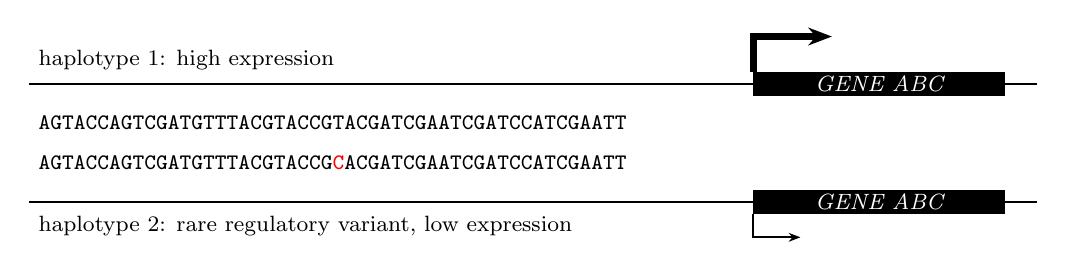
\begin{tikzpicture}[>=Stealth, every node/.style={font=\small}]
    \node[font=\ttfamily\footnotesize, anchor=west] (s1) at (0,0.25) {AGTACCAGTCGATGTTTACGTACCGTACGATCGAATCGATCCATCGAATT};
    \node[font=\ttfamily\footnotesize, anchor=west] (s2) at (0,-0.25) {AGTACCAGTCGATGTTTACGTACCG\textcolor{red}{C}ACGATCGAATCGATCCATCGAATT};
    \draw[thick] (0,0.75) -- (12.8,0.75);
    \draw[thick] (0,-0.75) -- (12.8,-0.75);
    \fill (9.2,0.6) rectangle (12.4,0.9); \node[white, font=\footnotesize\itshape] at (10.8,0.75) {GENE ABC};
    \fill (9.2,-0.9) rectangle (12.4,-0.6); \node[white, font=\footnotesize\itshape] at (10.8,-0.75) {GENE ABC};
    \draw[line width=2.5pt, -{Stealth[length=3mm]}] (9.2,0.9) -- (9.2,1.35) -- (10.2,1.35);
    \draw[line width=0.6pt, -{Stealth[length=1.5mm]}] (9.2,-0.9) -- (9.2,-1.2) -- (9.8,-1.2);
    \node[right, font=\footnotesize] at (0,1.05) {haplotype 1: high expression};
    \node[right, font=\footnotesize] at (0,-1.05) {haplotype 2: rare regulatory variant, low expression};
  \end{tikzpicture}
  \caption{A rare variant (red) in a regulatory element upstream of a gene reduces transcription from the haplotype that carries it. In RNA-seq this appears as reduced total expression and as allelic imbalance at heterozygous sites in the gene.}
  \label{fig:reg_variant}
\end{figure}

\subsection{Expression and splicing outliers}

An \emph{expression outlier} is a gene whose expression in the patient is extreme relative to a reference population, such as the GTEx samples of the same tissue. After normalizing expression and removing the effects of known covariates and hidden confounders (Chapter 12), the expression of gene $u$ in the patient is converted to a $z$-score, $z_u=(e_u-\bar e_u)/s_u$, with $\bar e_u$ and $s_u$ the mean and standard deviation of the normalized expression $e_u$ across the reference samples (Figure~\ref{fig:outliers}a). In GTEx, individuals who were expression outliers for a gene, particularly consistently across tissues, were enriched for rare variants near that gene, with the strongest enrichment for structural variants, frameshifts and splice-site variants~\citep{li2017}. Combining expression, splicing and allelic outlier signals with variant annotations improves the prioritization further~\citep{ferraro2020}.

A \emph{splicing outlier} is an aberrant splicing event: a splice junction that is used in the patient but rarely or never in controls, or a change in the relative usage of junctions (Figure~\ref{fig:outliers}b). Splicing quantification was the subject of Chapter 10. \citet{cummings2017} applied RNA-seq of muscle biopsies to patients with rare muscle disorders who remained undiagnosed after exome or genome sequencing, and found pathogenic exon skipping, exon extension and splice-site creation events absent from GTEx muscle samples, which established a diagnosis for a substantial fraction of the patients. Several of the causal variants were deep intronic or exonic changes whose effect on splicing had not been recognized from sequence.

\begin{figure}[!htbp]
  \centering
  \includegraphics[width=0.95\linewidth]{outliers.pdf}
  \caption{Outlier detection against a reference population of 500 simulated individuals. (a) Expression $z$-scores of one gene; the patient (red) has $z=-5.2$. (b) Fraction of reads at an exon that use a junction skipping it; the patient uses the skipping junction in 42\% of reads, against a few percent in the reference population.}
  \label{fig:outliers}
\end{figure}

\subsection{Allelic outliers}

Allele-specific expression (ASE), introduced in Chapter 12, gives a test within the patient: at a heterozygous site in a transcribed region, the reads from the two haplotypes can be counted, and an imbalance means that one haplotype is expressed more than the other. A rare regulatory variant or a nonsense-mediated decay trigger on one haplotype produces exactly this. The difficulty is that allelic imbalance is common. Most genes have common eQTLs, and in any individual, the two haplotypes of a gene often differ in expression for reasons unrelated to disease. A raw test of imbalance against $1/2$ flags thousands of genes per person.

ANEVA-DOT~\citep{mohammadi2019} addresses this by asking whether the imbalance is unusual \emph{for that gene}. Genes differ in how much regulatory variation the population tolerates. For a dosage-sensitive gene, selection keeps regulatory variants rare and their effects small, so the genetic variance of its expression is low; for a tolerant gene, large common eQTL effects are normal. ANEVA estimates this genetic variance, $V^G$, for each gene from ASE data in a reference population (GTEx). ANEVA-DOT then tests a patient's allelic counts against the distribution implied by $V^G$.

A simplified version of the model is as follows. Let $s\in\R$ be the log$_2$ ratio of the expression of haplotype 1 to haplotype 2 in an individual, the allelic fold change. In the population, $s\sim\Normal(0,V^G)$. Given $s$, a read comes from haplotype 1 with probability $\pi(s)=2^s/(1+2^s)$, and with $n$ reads at the site, the count $r$ from haplotype 1 is beta-binomial (Chapter 12), which allows for overdispersion from technical sources such as PCR duplicates,
\begin{equation}
  r\mid s \sim \operatorname{BetaBinomial}\big(n,\ c\,\pi(s),\ c\,(1-\pi(s))\big),
\end{equation}
where $c>0$ is a concentration parameter. Integrating over $s$ gives the null distribution of $r$ for a patient whose regulatory variation is typical of the population,
\begin{equation}
  P(r\mid n) = \int \Normal(s\mid 0, V^G)\,P(r\mid n,s)\,ds ,
\end{equation}
and the two-sided p-value of the observed count $r_{\text{obs}}$ is $2\min\{P(r\leq r_{\text{obs}}\mid n),P(r\geq r_{\text{obs}}\mid n)\}$. Figure~\ref{fig:aneva_dot} shows the same patient counts, 640 reads from one haplotype and 157 from the other, a four-fold imbalance, against two genes. For a gene with low $V^G$ the imbalance is far outside the population distribution ($p\approx 10^{-12}$); for a gene with high $V^G$ it is unremarkable ($p\approx 0.07$). The scale of what counts as an outlier is set by the population, gene by gene.

\begin{figure}[!htbp]
  \centering
  \includegraphics[width=0.9\linewidth]{aneva_dot.pdf}
  \caption{Allelic counts at a heterozygous site for 4000 simulated individuals (blue) drawn from the population model with low ($V^G=0.02$, left) and high ($V^G=1.2$, right) genetic variance of allelic fold change, total counts between 10 and 1600 and beta-binomial concentration $c=200$. Axes are on a square-root scale; the diagonal is allelic balance. The patient (red) has 640 and 157 reads from the two haplotypes; the p-values are from the marginal beta-binomial model. After the ANEVA-DOT analysis of \citet{mohammadi2019}.}
  \label{fig:aneva_dot}
\end{figure}

%======================================================================
\section{Learning gene impairment scores: DeepRVAT}
\label{sec:deeprvat}
%======================================================================

Every test in this chapter needs a rule for turning an individual's variants in a gene into evidence: which variants to include, how to weight them by frequency, and which annotations to trust. Burden tests and SKAT fix the rule in advance. The functional score test picks among a few candidate rules. DeepRVAT~\citep{clarke2024} learns the rule from data with a neural network, shared across genes and traits.

\subsection{A set function of variants}

Let $\mathcal{V}_{iu}$ be the set of rare variants that individual $i$ carries in gene $u$, and $\va_k\in\R^D$ the annotation vector of variant $k$. DeepRVAT used $D=34$ annotations: a transform of the MAF, predicted consequences (missense, stop gain, splice region and so on), protein-level scores (SIFT, PolyPhen-2, AlphaMissense, PrimateAI), CADD and ConDel, splicing predictions (SpliceAI, AbSplice), principal components of DeepSEA chromatin predictions, and predicted RNA-binding protein binding. The \emph{gene impairment score} of individual $i$ in gene $u$ is
\begin{equation}
  \psi(\mathcal{V}_{iu}) = \operatorname{logit}^{-1}\Big(\kappa\Big(\max_{k\in\mathcal{V}_{iu}}\phi(\va_k)\Big)\Big) \in (0,1),
  \label{eq:deeprvat}
\end{equation}
where $\phi:\R^D\to\R^H$ is a multilayer perceptron applied to each variant, the maximum is taken elementwise over the variants in the set, $\kappa:\R^H\to\R$ is a second multilayer perceptron, and $\operatorname{logit}^{-1}$ is the logistic function. (\citet{clarke2024} write $\rho$ for $\kappa$ and $f$ for the pooling operation.) The score is close to one if the gene is likely impaired and close to zero if the variants look benign.

Equation~\eqref{eq:deeprvat} is a \emph{deep set} architecture~\citep{zaheer2017}. The input is a set, with no natural order and variable size, so the function must be invariant to permutations of the variants. \citet{zaheer2017} showed that permutation-invariant functions of sets can be written as $\kappa(\sum_k\phi(\va_k))$ for suitable $\phi$ and $\kappa$; replacing the sum by an elementwise maximum keeps the invariance. The maximum has a natural interpretation here: one damaging variant is enough to impair a gene, and adding benign variants should not increase the score, which a sum would do. Each hidden unit of $\phi$ acts as a learned detector for one kind of damaging variant, and the maximum records whether any variant in the set triggers it.

\begin{figure}[!htbp]
  \centering
  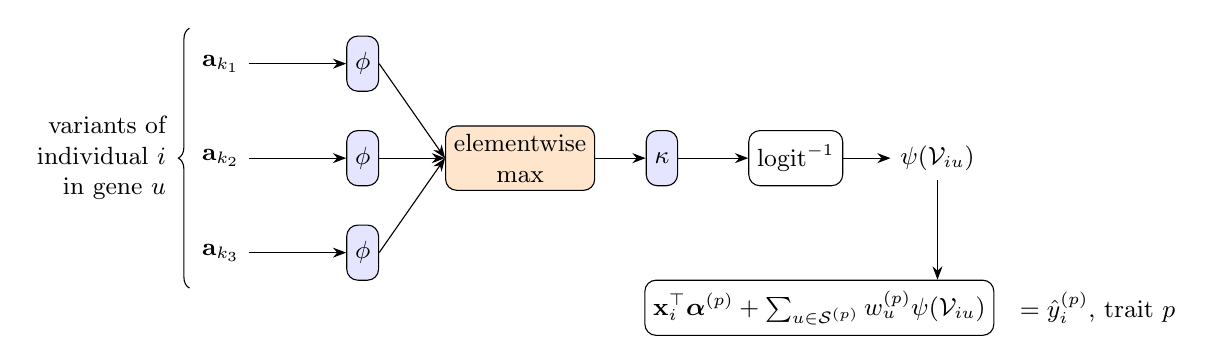
\begin{tikzpicture}[>=Stealth, every node/.style={font=\small},
      box/.style={draw, rounded corners, align=center, inner sep=3pt, minimum height=7mm}]
    \foreach \k/\y in {1/1.2, 2/0, 3/-1.2} {
      \node (a\k) at (0,\y) {$\va_{k_\k}$};
      \node[box, fill=blue!10] (p\k) at (1.8,\y) {$\phi$};
      \draw[->] (a\k) -- (p\k);
    }
    \node[box, fill=orange!20] (mx) at (3.8,0) {elementwise\\max};
    \foreach \k in {1,2,3} \draw[->] (p\k.east) -- (mx.west);
    \node[box, fill=blue!10] (rh) at (5.6,0) {$\kappa$};
    \node[box] (sg) at (7.3,0) {$\operatorname{logit}^{-1}$};
    \node (psi) at (9.1,0) {$\psi(\mathcal{V}_{iu})$};
    \draw[->] (mx) -- (rh); \draw[->] (rh) -- (sg); \draw[->] (sg) -- (psi);
    \node[box] (lin) at (7.6,-1.9) {$\vx_i^\top\valpha^{(p)}+\sum_{u\in\mathcal{S}^{(p)}}w_u^{(p)}\psi(\mathcal{V}_{iu})$};
    \draw[->] (psi) -- (psi |- lin.north);
    \node[right=2mm of lin] {$=\hat y_i^{(p)}$, trait $p$};
    \draw[decorate, decoration={brace, amplitude=4pt}] (-0.4,-1.65) -- (-0.4,1.65) node[midway, left=5pt, align=right] {variants of\\individual $i$\\in gene $u$};
  \end{tikzpicture}
  \caption{DeepRVAT. Each variant's annotations pass through a shared network $\phi$, the outputs are pooled by an elementwise maximum, and a second network $\kappa$ with a logistic output gives the gene impairment score $\psi$. During training, the scores of seed genes predict each trait through a linear model. After \citet{clarke2024}.}
  \label{fig:deeprvat}
\end{figure}

\subsection{Training and testing}

The score function is trained to predict traits. For trait $p$, with covariates $\vx_i$ (age, sex, genetic principal components) and coefficients $\valpha^{(p)}$, the prediction is
\begin{equation}
  \hat y_i^{(p)} = \vx_i^\top\valpha^{(p)} + \sum_{u\in\mathcal{S}^{(p)}} w_u^{(p)}\,\psi(\mathcal{V}_{iu}),
\end{equation}
where $\mathcal{S}^{(p)}$ is a set of \emph{seed genes} for trait $p$ and $w_u^{(p)}\in\R$ is a gene-specific coefficient. The networks $\phi$ and $\kappa$ are shared across all genes and all traits; only $\valpha^{(p)}$ and $w_u^{(p)}$ are specific to a trait. The loss is the squared error averaged over traits, minimized by stochastic gradient descent. The seed genes give the training signal. They were the genes significant in a conventional analysis that combines burden and SKAT tests of loss-of-function and missense variants with $\BetaD(1,25)$ weights. Training used 21 quantitative traits in about 160,000 exome-sequenced individuals from the UK Biobank. Sharing $\psi$ across traits means that what is learned about damaging variants from, say, lipid genes transfers to every other gene and trait. The score is ``trait-agnostic'', a learned, general-purpose definition of gene impairment.

For association testing, the trained $\psi$ is computed for every gene and individual and used as the burden score of Section~\ref{sec:burden}: for each gene $u$, the trait is regressed on $\psi(\mathcal{V}_{iu})$ and the covariates, and $H_0:\beta=0$ is tested with a score test. Genes outside the seed set can therefore be discovered. To avoid circularity, the model is trained with cross-validation: each individual's score is computed from models that were not trained on that individual. The seed genes themselves were chosen using the full data, so \citet{clarke2024} also checked the discoveries by replication in a larger UK Biobank release and on traits not used in training. Compared with burden and SKAT baselines, DeepRVAT found more significant gene-trait associations across the quantitative and binary traits it was applied to, and its scores improved the identification of individuals at high genetic risk.

DeepRVAT illustrates the trajectory of this chapter. A burden test hard-codes the prior that rare damaging variants matter; SKAT and the functional score test let the data choose among a few such priors; DeepRVAT learns the prior as a flexible function of annotations, with the statistical test kept simple so that its calibration is easy to check.

%======================================================================
\section{Summary}
%======================================================================

\begin{itemize}
  \item The power of a single-variant test depends on the sample size and MAF through approximately $Nf$, so rare variants need very large samples and de novo mutations cannot be tested individually. Rare variants can still have large effects, because selection keeps damaging variants rare.
  \item Burden tests aggregate the variants in a gene into a single score. They are powerful when most qualifying variants are causal with effects in the same direction, and depend on choices of frequency threshold, functional filter, controls and quality control. De novo mutations are tested against a mutation-rate model that accounts for sequence context such as CpG sites.
  \item Pathogenicity predictors include conservation scores, supervised and unsupervised combinations of annotations, and sequence models. LINSIGHT learns from the patterns of divergence and polymorphism that natural selection produces, with the prior probability of selection modelled as a function of genomic features.
  \item SKAT treats per-variant effects as random with mean zero and tests their variance component with a score statistic $\sum_jw_j^2S_j^2$ whose null distribution is a mixture of $\chi^2_1$ variables. It is robust to mixed effect directions. SKAT-O combines SKAT and burden through a correlation parameter $\rho$ and the minimum p-value over a grid.
  \item The functional score test adds one variance component per annotation and combines the resulting statistics, gaining power when annotations are informative and losing little when they are not.
  \item In autism, de novo noncoding mutations scored with deep learning sequence models and a classifier trained on known disease mutations have higher predicted impact in probands than in siblings. Network differential enrichment pools sparse mutations across functionally related genes, implicating synaptic and chromatin regulation genes. Reporter assays confirm that prioritized mutations alter regulatory activity.
  \item RNA-seq from patients reveals the consequences of rare variants as expression, splicing or allelic outliers, judged against a reference population, and ANEVA-DOT calibrates allelic imbalance by each gene's tolerance of regulatory variation.
  \item DeepRVAT learns a gene impairment score from variant annotations with a deep set network trained across traits, and uses it as the burden score in a conventional test.
\end{itemize}

%======================================================================
\section*{Exercises}
%======================================================================

\begin{enumerate}
  \item Using~\eqref{eq:ncp}, find the sample size needed for 80\% power at $\alpha=5\times10^{-8}$ to detect a variant with $f=10^{-3}$ and $\beta=0.25\sigma$. How does the answer change if the variant is ten times rarer?
  \item Starting from the marginal likelihood $\vy\sim\Normal(\mX\valpha,\sigma^2\mI+\tau\mG\mW\mR_\rho\mW\mG^\top)$, derive the score statistic~\eqref{eq:skat_q} and show that it equals $(1-\rho)Q_{\text{SKAT}}+\rho Q_{\text{burden}}$.
  \item Suppose a region has $M$ independent variants with equal weights and equal frequencies, half with effect $+\beta$ and half with effect $-\beta$. Show that the expected burden score statistic $\E[\vw^\top\vS]$ is zero under the alternative, while $\E[Q_{\text{SKAT}}]$ increases with $\beta^2$.
  \item For the simplified LINSIGHT likelihood~\eqref{eq:linsight_lik}, derive the gradient of $\log P(X_i)$ with respect to $\vw_\rho$, for the Gompertz link $g(x)=\exp(-3e^{-x})$. Show that sites with the pattern $\mathsf{D}$ always push $\rho_i$ down, and explain why monomorphic sites push it up only slightly.
  \item Show that the effective sample size $N=(\sum_ma_m)^2/\sum_ma_m^2$ satisfies $1\leq N\leq n$ for $n$ positive weights, with equality at the upper end only when all weights are equal.
  \item In the ANEVA-DOT model, show that without overdispersion ($c\to\infty$) and with $V^G\to 0$, the test reduces to a binomial test of $r$ against $n/2$. Why does this test flag far too many genes in practice?
  \item Explain why the elementwise maximum in~\eqref{eq:deeprvat} makes $\psi$ invariant to the order of the variants. Construct an example in which replacing the maximum by a sum would make a gene with many benign variants look more impaired than a gene with one damaging variant.
\end{enumerate}
.
\documentclass[11pt]{book}
\usepackage[T1]{fontenc}
\usepackage{lmodern}
\usepackage{microtype}
\usepackage[margin=1.1in]{geometry}
\usepackage{amsmath,amssymb,bm}
\usepackage{graphicx}
\usepackage{booktabs}
\usepackage{multirow}
\usepackage{xcolor}
\usepackage{caption}
\usepackage{subcaption}
\usepackage{algorithm}
\usepackage{algpseudocode}
\usepackage{tikz}
\usetikzlibrary{arrows.meta,positioning,calc,decorations.pathreplacing,decorations.pathmorphing,shapes.geometric,fit}
% HTML build only: tools/build_site.sh creates tikz-external.flag so that TeX also writes each
% tikzpicture to tikzext/main-figureN.pdf (TikZ external library); LaTeXML then shows those as images.
\IfFileExists{tikz-external.flag}{\usetikzlibrary{external}\tikzexternalize[prefix=tikzext/]}{}
\usepackage[numbers,sort&compress]{natbib}
\usepackage{hyperref}
\hypersetup{colorlinks=true,linkcolor=blue!50!black,citecolor=blue!50!black,urlcolor=blue!50!black}
\usepackage{etoc}
\makeatletter % wider number columns in contents lists, for numbers such as 11.11 and 11.11.10
\renewcommand*\l@section{\@dottedtocline{1}{1.5em}{3em}}
\renewcommand*\l@subsection{\@dottedtocline{2}{4.5em}{3.9em}}
\makeatother
% Contents list printed under each chapter heading (sections and subsections).
\newcommand{\chaptertoc}{%
  \begingroup
  \etocsettocstyle{\noindent\rule{\linewidth}{0.4pt}\par\smallskip\noindent\textbf{Contents of this chapter}\par\smallskip}{\noindent\rule{\linewidth}{0.4pt}\par\bigskip}%
  \etocsetnexttocdepth{subsection}%
  \localtableofcontents
  \endgroup}
\graphicspath{{figures/}}

\begin{document}
\setcounter{chapter}{12}
% Chapter 13: rare variants.
% Requires: amsmath, amssymb, bm, graphicx, booktabs, multirow, subcaption,
% tikz (arrows.meta, positioning, calc, decorations.pathreplacing, shapes.geometric, fit), natbib.
% Computed figures are produced by scripts/make_figures.py;
% figures/slides/ holds figures taken from the lecture slides.

\providecommand{\R}{\mathbb{R}}
\providecommand{\E}{\mathbb{E}}
\providecommand{\Normal}{\mathcal{N}}
\providecommand{\argmax}{\operatorname*{arg\,max}}
\providecommand{\argmin}{\operatorname*{arg\,min}}
\providecommand{\vy}{\mathbf{y}}
\providecommand{\vx}{\mathbf{x}}
\providecommand{\mX}{\mathbf{X}}
\providecommand{\mI}{\mathbf{I}}
\providecommand{\vb}{\boldsymbol{\beta}}
\providecommand{\veps}{\boldsymbol{\epsilon}}
\providecommand{\vp}{\mathbf{p}}
\providecommand{\vg}{\mathbf{g}}
\providecommand{\ind}{\mathbf{1}}
\providecommand{\valpha}{\boldsymbol{\alpha}}
\providecommand{\vz}{\mathbf{z}}
\providecommand{\va}{\mathbf{a}}
\providecommand{\vr}{\mathbf{r}}
\providecommand{\vmu}{\boldsymbol{\mu}}
\providecommand{\vphi}{\boldsymbol{\phi}}
\providecommand{\vw}{\mathbf{w}}
\providecommand{\vd}{\mathbf{d}}
\providecommand{\vc}{\mathbf{c}}
\providecommand{\vS}{\mathbf{S}}
\providecommand{\mG}{\mathbf{G}}
\providecommand{\mK}{\mathbf{K}}
\providecommand{\mW}{\mathbf{W}}
\providecommand{\mR}{\mathbf{R}}
\providecommand{\mP}{\mathbf{P}}
\providecommand{\mD}{\mathbf{D}}
\providecommand{\mV}{\mathbf{V}}
\providecommand{\mSigma}{\boldsymbol{\Sigma}}
\providecommand{\Var}{\operatorname{Var}}
\providecommand{\Cov}{\operatorname{Cov}}
\providecommand{\tr}{\operatorname{tr}}
\providecommand{\Bin}{\operatorname{Binomial}}
\providecommand{\BetaD}{\operatorname{Beta}}
\providecommand{\Pois}{\operatorname{Poisson}}

\chapter{Rare variants}
\label{ch:rare_variants}

Chapters 11 and 12 tested genetic variants one at a time for association with a disease, a quantitative trait or a molecular phenotype such as gene expression. That approach works for common variants, those whose minor allele is carried by at least a few percent of people. Most human genetic variants are rare, however, and some of the variants with the largest effects on disease are rare because natural selection keeps them that way. For variants carried by a handful of people, and for \emph{de novo} mutations, which are present in a single individual, a single-variant test has little or no power.

This chapter covers the methods developed for this setting. They rest on two ideas. The first is to aggregate: instead of testing each variant, test whether a gene or region carries more, or more damaging, variation in cases than in controls. This gives burden tests and the variance component tests SKAT and SKAT-O. The second is to use prior information about which variants are likely to matter. Pathogenicity predictors such as LINSIGHT, which learns from patterns of natural selection, and the deep learning models of regulatory sequence from Chapters 2 and 3 provide such information, and the functional score test and DeepRVAT build it into the association test. A case study of noncoding de novo mutations in autism shows these pieces used together, followed by network-based pathway analysis and experimental validation. The chapter ends with molecular data from patients: RNA-seq can reveal the consequences of a rare variant directly, as an expression, splicing or allelic outlier.

%======================================================================
\section{Why rare variants need different methods}
\label{sec:why_rare}
%======================================================================

\subsection{The allele frequency spectrum}

Recall from Chapter 11 that two unrelated people differ at roughly one position in every thousand. Each variable position, or single nucleotide polymorphism (SNP), usually has two alleles, and the \emph{minor allele frequency} (MAF) $f\in(0,0.5]$ is the frequency of the less common one. About three million SNPs per genome have $f\geq 5\%$ and are called common. Many more variants are rare. When large numbers of people are sequenced, the number of distinct variants keeps growing, and most newly found variants are seen in only one or a few individuals. The Genome Aggregation Database (gnomAD), which aggregated exome and genome sequences from 141,456 people~\citep{karczewski2020}, illustrates this: most of the variants it catalogues are rare, and a large fraction are \emph{singletons}, observed in a single person. A \emph{private} variant is found only in one family, and a \emph{de novo} mutation arose in a parent's germ cell, so that the child carries it and neither parent does. A typical genome carries around 70 de novo single nucleotide mutations.

\subsection{Effect size and allele frequency}

Effect sizes and allele frequencies are inversely related (Figure~\ref{fig:effect_freq})~\citep{manolio2009}. The variants that cause Mendelian diseases are rare and have large effects. The variants found by genome-wide association studies (GWAS) of common diseases are common and have small effects, with odds ratios typically below 1.5. Between these lie low-frequency variants of intermediate effect. Few common variants have large effects on common disease, and rare variants with small effects are very hard to find by genetic means at all.

The inverse relationship arises through natural selection. A variant that increases the risk of a disease that reduces the number of children its carriers have is selected against, and the stronger its effect, the more effectively selection keeps its frequency low. A variant of small effect is almost invisible to selection and can drift to high frequency. An exception is late-onset disease. Selection is blind to effects after reproductive age, which is one reason why alleles such as the \textit{APOE} $\varepsilon4$ allele, which increases the risk of Alzheimer's disease, remain common.

\begin{figure}[!htbp]
  \centering
  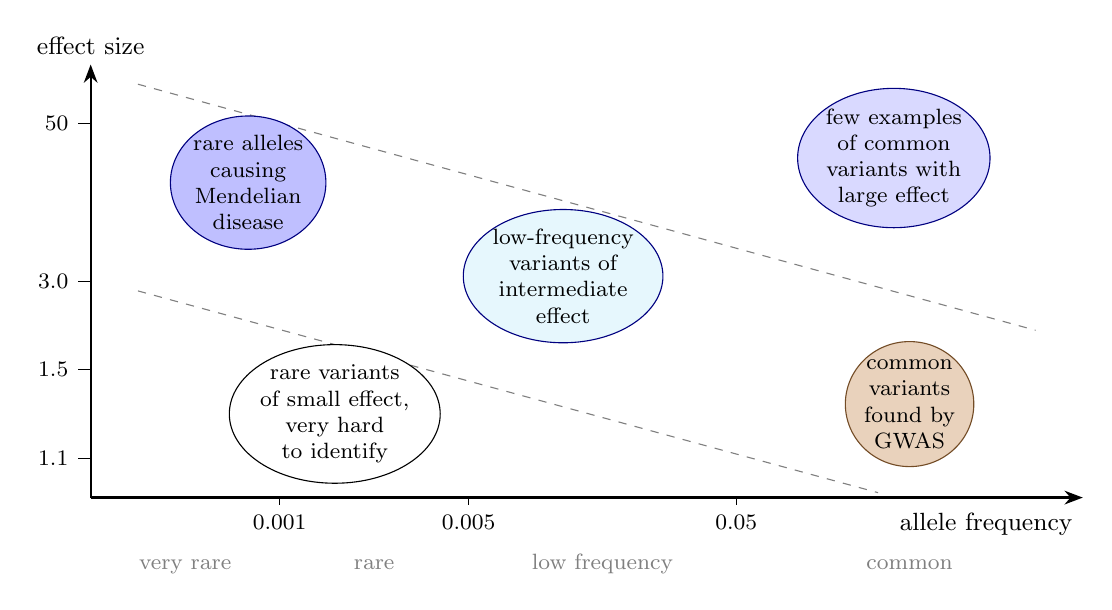
\begin{tikzpicture}[>=Stealth, every node/.style={font=\small}, x=2.0cm, y=1.25cm]
    \draw[->, thick] (0,0) -- (6.3,0) node[below left=2pt and 0pt, align=right] {allele frequency};
    \draw[->, thick] (0,0) -- (0,4.4) node[above] {effect size};
    \foreach \x/\l in {1.2/0.001, 2.4/0.005, 4.1/0.05} {
      \draw (\x,0) -- (\x,-0.08) node[below] {\footnotesize \l};
    }
    \node[below, font=\footnotesize, gray, text height=1.5ex, text depth=.25ex] at (0.6,-0.45) {very rare};
    \node[below, font=\footnotesize, gray, text height=1.5ex, text depth=.25ex] at (1.8,-0.45) {rare};
    \node[below, font=\footnotesize, gray, text height=1.5ex, text depth=.25ex] at (3.25,-0.45) {low frequency};
    \node[below, font=\footnotesize, gray, text height=1.5ex, text depth=.25ex] at (5.2,-0.45) {common};
    \foreach \y/\l in {0.4/1.1, 1.3/1.5, 2.2/3.0, 3.8/50} {
      \draw (0,\y) -- (-0.08,\y) node[left] {\footnotesize \l};
    }
    \draw[dashed, gray] (0.3,4.2) -- (6.0,1.7);
    \draw[dashed, gray] (0.3,2.1) -- (5.0,0.05);
    \tikzset{blob/.style={ellipse, draw, align=center, font=\footnotesize, inner sep=0pt}}
    \node[blob, fill=blue!25, draw=blue!50!black] at (1.0,3.2) {rare alleles\\causing\\Mendelian\\disease};
    \node[blob, fill=cyan!10, draw=blue!50!black] at (3.0,2.25) {low-frequency\\variants of\\intermediate\\effect};
    \node[blob, fill=brown!35, draw=brown!60!black] at (5.2,0.95) {common\\variants\\found by\\GWAS};
    \node[blob, fill=blue!15, draw=blue!50!black] at (5.1,3.45) {few examples\\of common\\variants with\\large effect};
    \node[blob, fill=white, draw=black] at (1.55,0.85) {rare variants\\of small effect,\\very hard\\to identify};
  \end{tikzpicture}
  \caption{Effect size (odds ratio, log scale) against risk allele frequency. Most known associations lie between the dashed lines. Redrawn after \citet{manolio2009}.}
  \label{fig:effect_freq}
\end{figure}

\subsection{Power of a single-variant test}
\label{sec:power}

Consider a quantitative trait and a single variant. Let $N$ be the number of individuals, $g_i\in\{0,1,2\}$ the number of copies of the minor allele carried by individual $i$, and $y_i\in\R$ the trait. The additive model from Chapter 11 is
\begin{equation}
  y_i = \mu + \beta g_i + \epsilon_i, \qquad \epsilon_i\overset{\text{iid}}{\sim}\Normal(0,\sigma^2),
\end{equation}
with intercept $\mu$, per-allele effect $\beta\in\R$ and noise variance $\sigma^2$. The least-squares estimate is $\hat\beta=\sum_i(g_i-\bar g)(y_i-\bar y)/\sum_i(g_i-\bar g)^2$, with variance $\sigma^2/\sum_i(g_i-\bar g)^2$. Under Hardy-Weinberg equilibrium $g_i\sim\Bin(2,f)$, so $\Var(g_i)=2f(1-f)$ and $\sum_i(g_i-\bar g)^2\approx 2Nf(1-f)$. The test statistic $z=\hat\beta/\operatorname{se}(\hat\beta)$ is then approximately normal with unit variance and mean
\begin{equation}
  \E[z] \approx \frac{\beta}{\sigma}\sqrt{2Nf(1-f)} .
  \label{eq:ncp}
\end{equation}
For a two-sided test at level $\alpha$ with critical value $z_{\alpha/2}$, the power, the probability of detecting the association when it is real, is
\begin{equation}
  \text{power} = \Phi\left(\E[z]-z_{\alpha/2}\right) + \Phi\left(-\E[z]-z_{\alpha/2}\right),
\end{equation}
where $\Phi$ is the standard normal cumulative distribution function. For rare variants $1-f\approx 1$, so power depends on the sample size and allele frequency only through $Nf$, which is half the expected number of minor alleles in the sample, and on the standardized effect $\beta/\sigma$. Halving the allele frequency requires doubling the sample size for the same power.

Figure~\ref{fig:power_single} shows the consequence at the genome-wide threshold $\alpha=5\times10^{-8}$. With $10^5$ individuals, a variant with a large effect, half a standard deviation per allele, is detected reliably down to a MAF of about $10^{-3}$, but a variant with a modest effect of $0.1\sigma$ needs a MAF of a few percent. Variants with $f=10^{-5}$ are out of reach even with a million people. For a de novo mutation, $Nf$ is effectively one: the variant is carried by one person, and no sample size will make a single-variant test informative.

\begin{figure}[!htbp]
  \centering
  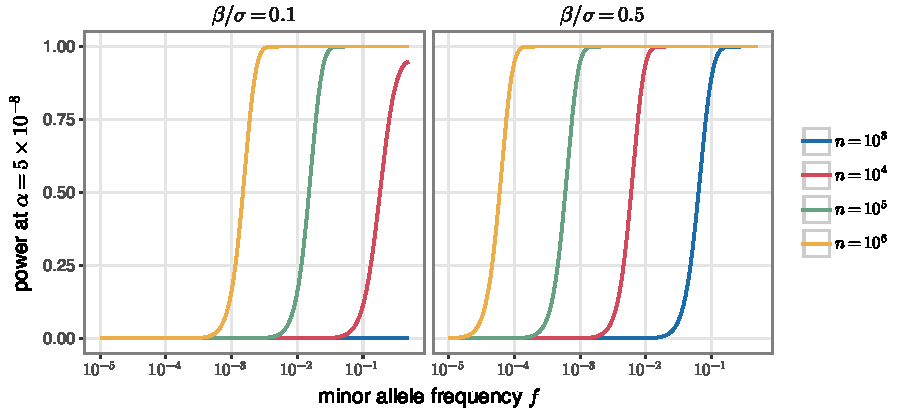
\includegraphics[width=0.9\linewidth]{power_single_variant.pdf}
  \caption{Power of a single-variant additive test at $\alpha=5\times10^{-8}$ as a function of MAF, for sample sizes from $10^3$ to $10^6$ and two standardized effect sizes. Power depends on $N$ and $f$ through approximately $Nf$, so the curves are shifted copies on the log scale. Computed from~\eqref{eq:ncp}.}
  \label{fig:power_single}
\end{figure}

Two strategies follow. Since we cannot test each rare variant on its own, we \emph{aggregate} variants within a unit, usually a gene, and test the unit. And since aggregation dilutes the signal with neutral variants, we use \emph{prior information} to pick out, or upweight, the variants likely to be functional.

%======================================================================
\section{Burden tests}
\label{sec:burden}
%======================================================================

A burden test asks whether a gene carries more variants, or more damaging variants, in affected individuals than expected by chance. Let a gene or region contain $M$ variants that pass some filter, for example $f_j<1\%$ and a predicted loss of function. Let $\mG\in\{0,1,2\}^{N\times M}$ be the genotype matrix, with $G_{ij}$ the number of minor alleles of variant $j$ carried by individual $i$, and let $\vw\in\R^M_{\geq 0}$ be a vector of variant weights. The \emph{burden score} of individual $i$ is
\begin{equation}
  C_i = \sum_{j=1}^M w_j G_{ij} .
\end{equation}
Early versions collapse the variants into an indicator of carrying any qualifying variant, $C_i=\ind[\sum_j G_{ij}>0]$~\citep{morgenthaler2007, li2008}, or weight each variant by $w_j=1/\sqrt{f_j(1-f_j)}$, so that rarer variants count for more~\citep{madsen2009}. The burden score then replaces the genotype in a regression. With covariates $\vx_i\in\R^{C}$ (for example age, sex and genetic principal components), coefficients $\valpha\in\R^C$ and mean $\mu_i=\E[y_i]$,
\begin{equation}
  h(\mu_i) = \vx_i^\top\valpha + C_i\beta ,
  \label{eq:burden_glm}
\end{equation}
where $h$ is the identity for a quantitative trait and the logit for a binary trait. The test of $H_0:\beta=0$ is a single-degree-of-freedom test, so it is as cheap as testing one common variant.

The burden model is the per-variant model $h(\mu_i)=\vx_i^\top\valpha+\sum_j G_{ij}\beta_j$ with the constraint $\beta_j=w_j\beta$. It assumes that every qualifying variant has an effect, in the same direction, of size proportional to its weight. When this holds, pooling the variants concentrates their signal into one statistic. When it does not, the test loses power: neutral variants add noise to $C_i$, and variants with opposite effects cancel.

\subsection{The score test}

The tests in this chapter are \emph{score tests}, which need only the model fitted under the null hypothesis. For a quantitative trait, fit $y_i=\vx_i^\top\valpha+\epsilon_i$ by least squares and let $\hat\mu_i=\vx_i^\top\hat\valpha$ be the fitted values. The score for $\beta$ at $\beta=0$ is the derivative of the log likelihood, $\sigma^{-2}\sum_i C_i(y_i-\hat\mu_i)$. Define the score statistic of variant $j$ as
\begin{equation}
  S_j = \sum_{i=1}^N G_{ij}(y_i-\hat\mu_i), \qquad \vS = \mG^\top(\vy-\hat\vmu)\in\R^M ,
  \label{eq:score}
\end{equation}
so that the burden score is $\sum_i C_i(y_i-\hat\mu_i)=\vw^\top\vS$. Let $\mP_0=\mI-\mX(\mX^\top\mX)^{-1}\mX^\top$ be the $N\times N$ projection onto the residual space of the covariate matrix $\mX\in\R^{N\times C}$. The residuals are $\vy-\hat\vmu=\mP_0\vy$, and under $H_0$ they are distributed as $\Normal(\mathbf{0},\sigma^2\mP_0)$, since $\mP_0$ is symmetric and idempotent. It follows that
\begin{equation}
  \vS\sim\Normal\left(\mathbf{0},\ \sigma^2\mG^\top\mP_0\mG\right), \qquad
  Q_{\text{burden}} = \frac{(\vw^\top\vS)^2}{\hat\sigma^2\,\vw^\top\mG^\top\mP_0\mG\vw} \sim \chi^2_1 .
\end{equation}
For a binary trait fitted by logistic regression the same holds with $\sigma^2\mI$ replaced by $\mV=\operatorname{diag}(\hat\mu_i(1-\hat\mu_i))$ and $\mP_0$ by its weighted version. The vector $\vS$ and its covariance are \emph{summary statistics}: studies can share them without sharing genotypes, and they can be combined across studies by adding them, which makes the tests below suitable for meta-analysis.

\subsection{Counting tests and de novo mutations}

In a case-control study, the simplest burden test counts carriers. Let $a$ of $N_1$ cases and $b$ of $N_0$ controls carry a qualifying variant in the gene. Fisher's exact test on the $2\times 2$ table of carrier status against disease status tests whether the carrier proportions differ.

For de novo mutations the comparison is against a mutation model rather than controls. Sequencing parent-child trios identifies the mutations each child carries that neither parent does. Let $T$ be the number of trios and $\mu_g$ the per-generation probability that a new mutation of a given class (for example protein-truncating) arises in gene $g$ on one haploid genome. Each child receives two haploid genomes, so the expected number of de novo mutations in gene $g$ across the cohort is $\lambda_g=2T\mu_g$, and the number observed, $k_g$, is approximately Poisson distributed under the null hypothesis that the gene plays no role in the disease. The p-value is
\begin{equation}
  P(K\geq k_g) = 1-\sum_{k=0}^{k_g-1}\frac{\lambda_g^k e^{-\lambda_g}}{k!}, \qquad K\sim\Pois(\lambda_g).
\end{equation}
The mutation rate $\mu_g$ must be modelled carefully, because some positions mutate much more often than others. The cytosine of a CpG dinucleotide is usually methylated, and methylated cytosine deaminates spontaneously to thymine, so CG$\to$TG changes occur roughly an order of magnitude more often than other transitions. Gene-level rates are therefore computed by summing per-site probabilities that depend on the sequence context, typically the trinucleotide around each site~\citep{samocha2014}. A gene with many CpGs, or a long gene, is expected to receive more mutations by chance.

\subsection{Practical choices}

A burden analysis involves several choices, each of which can make or break it.
\begin{itemize}
  \item \emph{Which variants qualify.} A MAF threshold (1\%, 0.1\%, singletons only) and a functional filter: protein-truncating variants only, or also missense variants predicted to be damaging, and if so by which predictor (Section~\ref{sec:pathogenicity}). Including more variants adds signal if they are functional and noise if not.
  \item \emph{Missing data.} Sequencing coverage varies across the genome and between samples. A variant can be absent from a sample because it is not there or because the site was not sequenced well enough to call it. If coverage differs between cases and controls, for example because they were sequenced at different centres, the difference alone creates spurious burden.
  \item \emph{Controls.} Sequencing controls is expensive, so it is tempting to compare cases with public databases such as gnomAD~\citep{karczewski2020}, which report allele counts for well over a hundred thousand individuals. TRAPD~\citep{guo2018} does this for exome data: it restricts the comparison to sites that are well covered in both data sets, applies matched quality filters, and calibrates the test using synonymous variants, which should show no excess in cases. Differences in sequencing technology, variant calling and ancestry between cases and public controls remain the main source of false positives.
\end{itemize}

Population data also tell us which genes tolerate damaging variation. For each gene, gnomAD compares the number of protein-truncating (loss-of-function, LoF) variants observed in the population with the number expected under a mutation model like the one above. A gene in which far fewer LoF variants are seen than expected is under strong selection: losing one copy is harmful enough that carriers have fewer children. The upper bound of the confidence interval on the observed/expected ratio (LOEUF) summarizes this constraint~\citep{karczewski2020}. Restricting a burden test to LoF-intolerant genes, or upweighting them, enriches for genes where a new damaging variant is likely to cause disease. We will see this in Section~\ref{sec:autism}.

%======================================================================
\section{Predicting pathogenicity}
\label{sec:pathogenicity}
%======================================================================

Burden tests need to know which variants to include, and every method in this chapter benefits from knowing which variants are likely to be functional. For protein-coding variants we have the genetic code: a premature stop codon or frameshift usually destroys the protein, a missense variant changes one amino acid, and a synonymous variant changes none, although it can still alter splicing (Chapter 10). Most of the genome is noncoding, and there the question of which variants matter is much harder. Pathogenicity predictors fall into a few families.
\begin{itemize}
  \item \emph{Conservation scores} measure how much a position has changed across species. phyloP~\citep{pollard2010} tests each position for slower (or faster) evolution than expected under neutrality on a phylogeny of many species; phastCons~\citep{siepel2005} uses a phylogenetic hidden Markov model (Chapter 6) to find conserved elements; GERP++~\citep{davydov2010} counts ``rejected substitutions''. Conservation is informative but misses functional elements that are specific to humans or primates, and regulatory elements turn over fast in evolution.
  \item \emph{Supervised combinations of annotations.} CADD~\citep{kircher2014} trains a classifier, originally a linear support vector machine, to distinguish variants that became fixed in the human lineage since the human-chimpanzee ancestor, which have survived selection and are mostly benign, from simulated de novo variants, which include deleterious ones in their natural proportion. Its features are many annotations, including conservation, regulatory marks and gene models. FunSeq2~\citep{fu2014} scores noncoding variants by combining conservation, regulatory annotations and network information.
  \item \emph{Unsupervised combinations.} Eigen~\citep{ionitalaza2016} combines many annotations without labelled variants. Its simplest variant, Eigen-PC, scores a variant by the projection of its annotations onto the leading eigenvector of their correlation matrix.
  \item \emph{Sequence models.} Deep learning models such as DeepSEA~\citep{zhou2015} (Chapter 2) predict chromatin features from sequence and so can score the effect of any variant, including variants never seen before, by comparing predictions for the two alleles.
\end{itemize}
A recurring problem is the lack of labels. There are few confirmed pathogenic noncoding variants, and those we have are biased towards particular regions, such as promoters of known disease genes. LINSIGHT avoids labelled variants altogether by learning from the signature that natural selection leaves in population and comparative genomic data.

\subsection{LINSIGHT}

LINSIGHT~\citep{huang2017} combines a generalized linear model of genomic features with INSIGHT, a probabilistic model of molecular evolution~\citep{gronau2013}. Its predecessor fitCons~\citep{gulko2015} grouped sites by their pattern of functional genomic marks and fitted INSIGHT to each group; LINSIGHT replaces the groups with a linear model, which scales to many features and gives a score for each site.

The data are of two kinds (Figure~\ref{fig:linsight_model}). Polymorphism data come from human genomes (54 unrelated individuals in the original study) and record, for each site, whether it is variable in humans and at what frequency. Divergence data come from outgroup primate genomes (chimpanzee, orangutan and rhesus macaque), which, through a phylogenetic model, give the probable ancestral allele and whether the human lineage has acquired a substitution since the ancestor. Natural selection changes both. At a site under purifying selection, new mutations are removed, so we expect fewer substitutions, fewer polymorphisms, and those polymorphisms that exist to be at low frequency, because harmful alleles do not drift to high frequency. A neutral site accumulates substitutions and polymorphisms at the background rate, with the neutral distribution of allele frequencies. The neutral rates vary along the genome with local mutation rate and genealogy, so they are estimated from flanking regions assumed to be neutral.

\begin{figure}[!htbp]
  \centering
  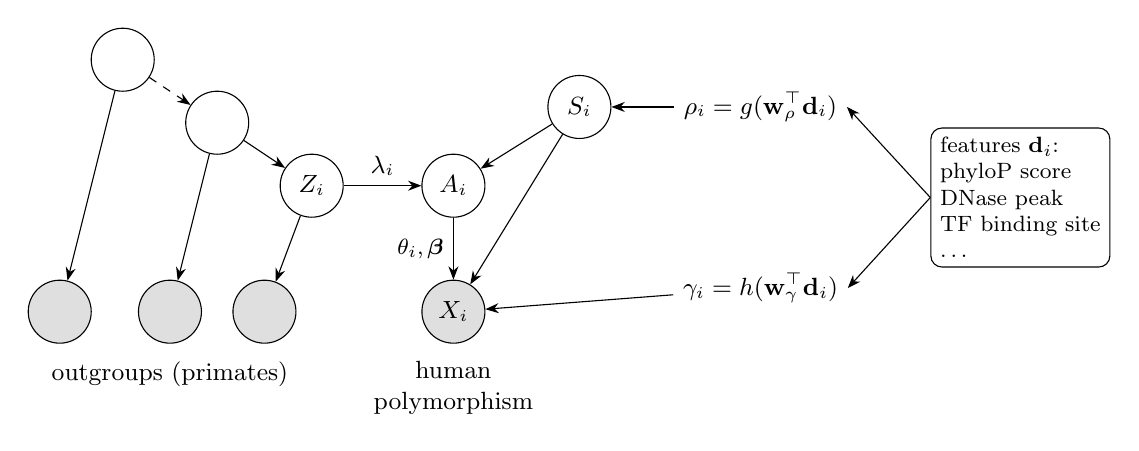
\begin{tikzpicture}[>=Stealth, every node/.style={font=\small},
      lat/.style={circle, draw, minimum size=8mm, inner sep=0pt},
      obs/.style={circle, draw, fill=gray!25, minimum size=8mm, inner sep=0pt},
      det/.style={diamond, draw, aspect=1, inner sep=1.5pt}]
    % outgroup tree
    \node[lat] (r) at (0,3.2) {};
    \node[lat] (n2) at (1.2,2.4) {};
    \node[lat] (Z) at (2.4,1.6) {$Z_i$};
    \node[obs] (o1) at (-0.8,0) {};
    \node[obs] (o2) at (0.6,0) {};
    \node[obs] (o3) at (1.8,0) {};
    \draw[->] (r) -- (o1); \draw[->, dashed] (r) -- (n2); \draw[->] (n2) -- (o2); \draw[->] (Z) -- (o3);
    \draw[->] (n2) -- (Z);
    \node[below=1mm of o2, align=center] {outgroups (primates)};
    \node[lat] (A) at (4.2,1.6) {$A_i$};
    \node[obs] (X) at (4.2,0) {$X_i$};
    \node[below=1mm of X, align=center] {human\\polymorphism};
    \draw[->] (Z) -- node[above] {$\lambda_i$} (A);
    \draw[->] (A) -- node[left, font=\footnotesize] {$\theta_i,\boldsymbol\beta$} (X);
    \node[lat] (Si) at (5.8,2.6) {$S_i$};
    \draw[->] (Si) -- (A); \draw[->] (Si) -- (X);
    \node (rho) at (8.1,2.6) {$\rho_i=g(\vw_\rho^\top\vd_i)$};
    \node (gam) at (8.1,0.3) {$\gamma_i=h(\vw_\gamma^\top\vd_i)$};
    \draw[->] (rho) -- (Si); \draw[->] (gam) -- (X);
    \node[draw, rounded corners, align=left, font=\footnotesize] (feat) at (11.4,1.45) {features $\vd_i$:\\phyloP score\\DNase peak\\TF binding site\\\dots};
    \draw[->] (feat.west) -- (rho.east); \draw[->] (feat.west) -- (gam.east);
  \end{tikzpicture}
  \caption{The LINSIGHT model for site $i$. Grey nodes are observed. Outgroup sequences inform the human-chimpanzee ancestral allele $Z_i$ and, with the neutral divergence rate $\lambda_i$, the human ancestral allele $A_i$. The observed human polymorphism data $X_i$ depend on the neutral polymorphism rate $\theta_i$, the neutral frequency spectrum $\boldsymbol\beta$ and the selection indicator $S_i$. The prior probability of selection $\rho_i$ and the relative rate of low-frequency polymorphism under selection $\gamma_i$ are functions of genomic features $\vd_i$. Redrawn after \citet{huang2017}.}
  \label{fig:linsight_model}
\end{figure}

Table~\ref{tab:linsight} lists the quantities in the model. For site $i$, the binary variable $S_i$ indicates whether the site is under selection, with prior probability $\rho_i$. To see how the likelihood works, assume the ancestral allele is known and classify the human data at site $i$ into five patterns: monomorphic with the ancestral allele ($\mathsf{M}$); monomorphic with a derived allele, that is, a substitution on the human lineage ($\mathsf{D}$); or polymorphic with the derived allele at low ($\mathsf{L}$), intermediate ($\mathsf{I}$) or high ($\mathsf{H}$) frequency. Under neutrality a polymorphism occurs with probability $\theta_i$ and its derived allele frequency falls into the three classes with probabilities $\boldsymbol\beta=(\beta_1,\beta_2,\beta_3)$, and a substitution occurs with probability $\lambda_i$. Under selection, substitutions and intermediate- or high-frequency polymorphisms are not allowed, and low-frequency polymorphisms occur at a rate reduced by the factor $\gamma_i$. This gives
\begin{center}
  \begin{tabular}{lcc}
    \toprule
    pattern $X_i$ & $P(X_i\mid S_i=0)$, neutral & $P(X_i\mid S_i=1)$, selected \\
    \midrule
    $\mathsf{M}$, monomorphic, ancestral & $(1-\theta_i)(1-\lambda_i)$ & $1-\gamma_i\theta_i$ \\
    $\mathsf{D}$, substitution & $(1-\theta_i)\lambda_i$ & $0$ \\
    $\mathsf{L}$, low-frequency derived & $\theta_i\beta_1$ & $\gamma_i\theta_i$ \\
    $\mathsf{I}$, intermediate-frequency derived & $\theta_i\beta_2$ & $0$ \\
    $\mathsf{H}$, high-frequency derived & $\theta_i\beta_3$ & $0$ \\
    \bottomrule
  \end{tabular}
\end{center}
Each column sums to one. INSIGHT also allows adaptive substitutions under selection; LINSIGHT drops this term because positive selection has a negligible effect at the genome-wide scale. The full model integrates over the uncertain ancestral allele with the outgroup phylogeny, and defines frequency classes by a threshold on the minor allele frequency, which complicates the expressions without changing their logic. Marginalizing over $S_i$, the likelihood of site $i$ is
\begin{equation}
  P(X_i) = \rho_i\,P(X_i\mid S_i=1) + (1-\rho_i)\,P(X_i\mid S_i=0) .
  \label{eq:linsight_lik}
\end{equation}

\begin{table}[!htbp]
  \centering
  \caption{Quantities in the LINSIGHT model, after \citet{huang2017}.}
  \label{tab:linsight}
  \begin{tabular}{lp{0.68\linewidth}}
    \toprule
    \multicolumn{2}{l}{\emph{Parameters inherited from INSIGHT}} \\
    $\rho_i$ & probability that site $i$ is under selection; the LINSIGHT score of site $i$ \\
    $\gamma_i$ & expected relative rate of low-frequency derived alleles at site $i$ given that it is under selection \\
    $\lambda_i$ & neutral substitution (divergence) rate at site $i$ \\
    $\theta_i$ & neutral polymorphism rate at site $i$ \\
    $\boldsymbol\beta=(\beta_1,\beta_2,\beta_3)$ & fractions of neutral polymorphisms with low-, intermediate- and high-frequency derived alleles \\
    \midrule
    \multicolumn{2}{l}{\emph{Variables inherited from INSIGHT}} \\
    $X_i$ & observed polymorphism data at site $i$: major allele, minor allele and minor allele frequency class \\
    $Z_i$ & human-chimpanzee ancestral allele at site $i$ \\
    $A_i$ & human ancestral allele at site $i$ \\
    $S_i$ & indicator of whether site $i$ is under selection \\
    \midrule
    \multicolumn{2}{l}{\emph{Components of the generalized linear model}} \\
    $\vd_i\in\R^m$ & genomic feature vector of site $i$ \\
    $\vw_\rho\in\R^m$ & weight vector for $\rho$ (free parameters) \\
    $\vw_\gamma\in\R^m$ & weight vector for $\gamma$ (free parameters) \\
    \bottomrule
  \end{tabular}
\end{table}

A single site carries almost no information: nearly all sites are monomorphic in a sample of a few dozen genomes, whether selected or not. INSIGHT obtained information by pooling many sites of the same type and estimating one $\rho$ for the group. LINSIGHT pools through features instead. Let $\vd_i\in\R^m$ be the feature vector of site $i$, including an intercept; the original model used $m=48$ features in three classes, conservation scores (phyloP, phastCons and others), predicted binding sites (transcription factor and microRNA binding sites, splice sites) and regional annotations (ChIP-seq, DNase-seq and histone modification peaks, enhancer annotations, distance to the nearest transcription start site). The two selection parameters are
\begin{equation}
  \rho_i = g(\vw_\rho^\top\vd_i), \qquad \gamma_i = h(\vw_\gamma^\top\vd_i),
\end{equation}
with weight vectors $\vw_\rho,\vw_\gamma\in\R^m$. The link $h$ is the logistic function. For $g$, LINSIGHT uses the asymmetric Gompertz function $g(x)=\exp(-3e^{-x})$, which, unlike the logistic, keeps the gradient from vanishing when $\rho_i$ is close to zero, as it is at most sites. The neutral parameters $\lambda_i$, $\theta_i$ and $\boldsymbol\beta$ are estimated beforehand from the flanking neutral regions and held fixed. The weights maximize the log likelihood $\sum_i\log P(X_i)$ over all noncoding sites in the genome, billions of terms, which is done by stochastic gradient ascent on minibatches of sites (Chapter 2). The model is a generalized linear model whose ``response'' $X_i$ is linked to the linear predictor through the mixture~\eqref{eq:linsight_lik} rather than through a standard exponential family.

The LINSIGHT score of a site is $\rho_i$, the \emph{prior} probability of selection given its features, not the posterior $P(S_i=1\mid X_i)$. This is deliberate: the score of a site should not depend on whether a polymorphism happens to have been observed there in 54 genomes, and the prior is defined for every site, including those where a patient carries a variant never seen before. Because $\rho_i$ is a probability that a mutation at site $i$ is selected against, it is also called the \emph{fitness consequence} of the site. Figure~\ref{fig:linsight_fitness}a shows that it behaves as expected across annotation classes: low for intergenic and intronic sites, higher for UTRs, promoters and binding sites, and highest at splice sites.

\begin{figure}[!htbp]
  \centering
  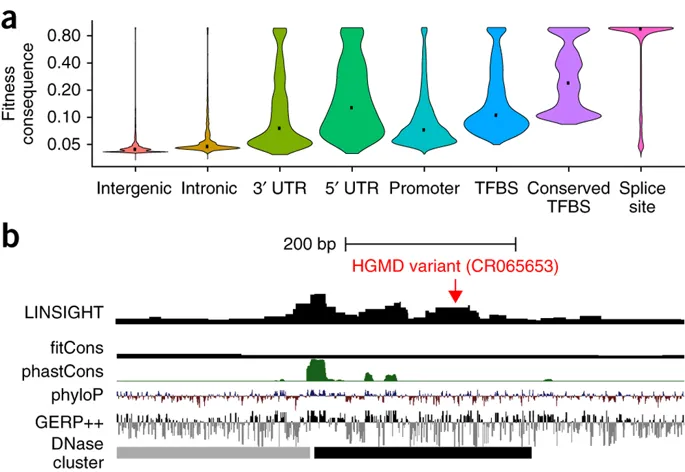
\includegraphics[width=0.75\linewidth]{slides/linsight_fitness.png}
  \caption{(a) Distribution of LINSIGHT scores (fitness consequence, log scale) of noncoding sites in different annotation classes. TFBS, transcription factor binding site. (b) LINSIGHT and other scores around a noncoding disease variant from the Human Gene Mutation Database. LINSIGHT is elevated across the DNase hypersensitive region containing the variant, whereas the conservation scores (phastCons, phyloP, GERP++) give little signal at the variant itself. Reproduced from \citet{huang2017}.}
  \label{fig:linsight_fitness}
\end{figure}

\subsection{Evaluating pathogenicity scores}

To evaluate a predictor we need variants of known effect. \citet{huang2017} used noncoding variants from the Human Gene Mutation Database (HGMD), which catalogues variants reported to cause inherited disease, and from ClinVar, as positives, and common SNPs (MAF $>1\%$) as negatives. The ROC curves (Chapter 1) in Figure~\ref{fig:linsight_roc} show LINSIGHT ahead of the alternatives, with phyloP, which uses conservation alone, the weakest. Two caveats apply to this kind of benchmark. Common variants are an easy negative set, since a variant that has risen to high frequency is unlikely to be strongly deleterious, so the task differs from the clinical one of distinguishing a pathogenic rare variant from a benign rare variant. The authors therefore also used negatives matched to the positives by distance to the transcription start site, or drawn from within 1 kb of each disease variant. And the positives are biased toward regions people have looked at, such as promoters of known disease genes, so methods that learn ``near a known disease gene'' are rewarded.

\begin{figure}[!htbp]
  \centering
  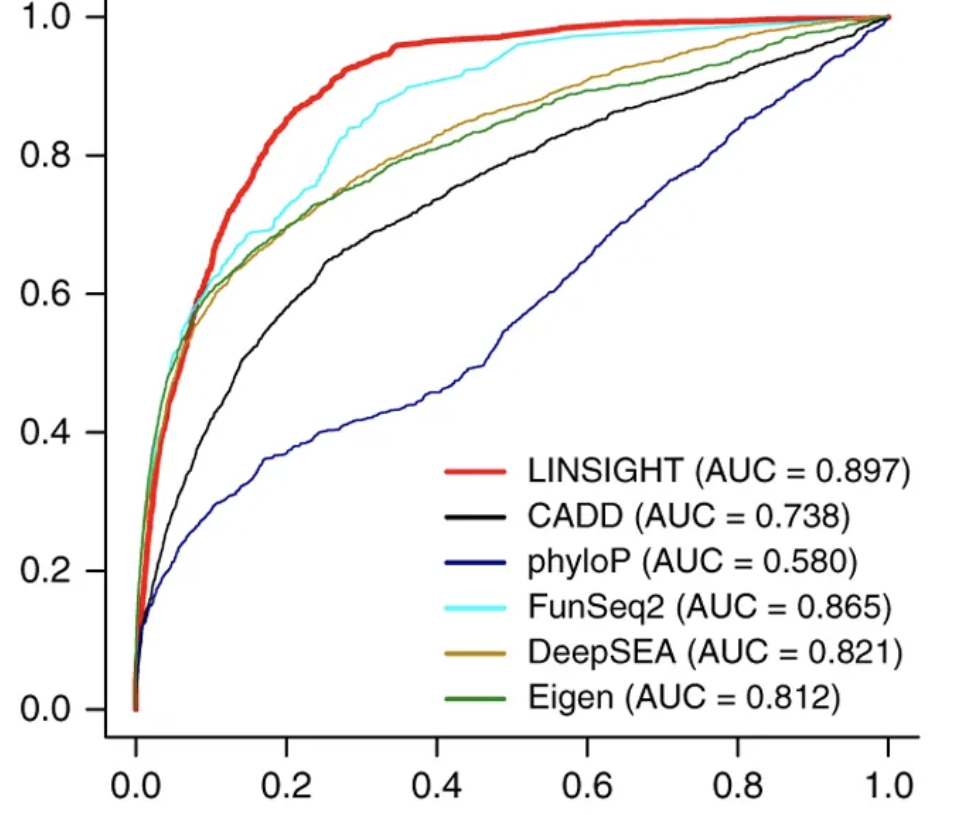
\includegraphics[width=0.5\linewidth]{slides/linsight_hgmd_roc.png}
  \caption{ROC curves (true positive rate against false positive rate) for distinguishing noncoding disease variants from HGMD from common SNPs not matched to the disease variants by location. phyloP, conservation across species; CADD, a classifier of observed against simulated variants; FunSeq2 and DeepSEA, see text; Eigen, an unsupervised combination of annotations. Reproduced from \citet{huang2017}.}
  \label{fig:linsight_roc}
\end{figure}

%======================================================================
\section{Variance component tests: SKAT and SKAT-O}
\label{sec:skat}
%======================================================================

Burden tests assume that all qualifying variants act in the same direction. This is reasonable for loss-of-function variants in a gene where losing one copy is harmful, but not in general. Some missense variants increase protein activity and others decrease it; in a regulatory region some variants increase expression and others decrease it; and most variants in a region may be neutral. The sequence kernel association test (SKAT)~\citep{wu2011} drops the assumption by treating the per-variant effects as random with mean zero, and SKAT-O~\citep{lee2012} interpolates between SKAT and the burden test.

\subsection{The model}

Let $\vg_i\in\{0,1,2\}^M$ be the genotypes of individual $i$ at the $M$ variants, so that $\vg_i^\top$ is row $i$ of $\mG$. The per-variant model is
\begin{equation}
  h(\mu_i) = \vx_i^\top\valpha + \vg_i^\top\vb, \qquad \vb\in\R^M,
\end{equation}
with $\vb$ random and
\begin{equation}
  \E[\beta_j]=0, \qquad \Var(\beta_j)=w_j^2\tau, \qquad \Cov(\beta_{j_1},\beta_{j_2})=\rho\,w_{j_1}w_{j_2}\tau \quad (j_1\neq j_2),
  \label{eq:skat_prior}
\end{equation}
where $\tau\geq 0$ is a variance component, $w_j$ is the weight of variant $j$ and $\rho\in[0,1]$ is the correlation between effects. In matrix form, $\Cov(\vb)=\tau\mW\mR_\rho\mW$, with $\mW=\operatorname{diag}(\vw)$ and $\mR_\rho=(1-\rho)\mI_M+\rho\ind\ind^\top$, where $\ind$ is the vector of $M$ ones. Two cases are of interest. With $\rho=0$ the effects are independent, with random signs and magnitudes that scale with $w_j$; this is SKAT, also called a \emph{dispersion} test, because it detects effects that spread the trait in either direction. With $\rho=1$ the effects are perfectly correlated, so $\vb=\vw\beta_0$ for a single random $\beta_0$ with variance $\tau$, which is the burden model~\eqref{eq:burden_glm}. The null hypothesis $\vb=\mathbf{0}$ becomes $H_0:\tau=0$, a test of one parameter however many variants the region contains.

\subsection{Deriving the score statistic}

For a quantitative trait with Gaussian noise, take $\vb$ to be Gaussian as well. Then $\vb$ can be integrated out, as for ridge regression in Chapter 1, and
\begin{equation}
  \vy\sim\Normal\left(\mX\valpha,\ \mSigma(\tau)\right), \qquad \mSigma(\tau) = \sigma^2\mI_N + \tau\mK, \qquad \mK = \mG\mW\mR_\rho\mW\mG^\top ,
\end{equation}
where $\mK\in\R^{N\times N}$ is a kernel matrix: $K_{ii'}$ measures the weighted genetic similarity of individuals $i$ and $i'$ in the region. Let $\vr=\vy-\mX\valpha$. The log likelihood is $\ell(\tau)=-\frac{1}{2}\log|\mSigma(\tau)|-\frac{1}{2}\vr^\top\mSigma(\tau)^{-1}\vr+\text{const}$. Using $\partial\log|\mSigma|/\partial\tau=\tr(\mSigma^{-1}\partial\mSigma/\partial\tau)$ and $\partial\mSigma^{-1}/\partial\tau=-\mSigma^{-1}(\partial\mSigma/\partial\tau)\mSigma^{-1}$, with $\partial\mSigma/\partial\tau=\mK$,
\begin{equation}
  \frac{\partial\ell}{\partial\tau} = -\frac{1}{2}\tr\left(\mSigma^{-1}\mK\right) + \frac{1}{2}\vr^\top\mSigma^{-1}\mK\mSigma^{-1}\vr .
\end{equation}
At $\tau=0$, $\mSigma=\sigma^2\mI$ and
\begin{equation}
  \left.\frac{\partial\ell}{\partial\tau}\right|_{\tau=0} = \frac{1}{2\sigma^4}\vr^\top\mK\vr - \frac{1}{2\sigma^2}\tr(\mK) .
\end{equation}
The trace term does not depend on the data, so the test can be based on the quadratic form in the residuals $\hat\vr=\vy-\mX\hat\valpha$ from the null model. Substituting $\mK$ and the score vector $\vS=\mG^\top\hat\vr$ from~\eqref{eq:score},
\begin{equation}
  Q_\rho = \hat\vr^\top\mK\hat\vr = \vS^\top\mW\mR_\rho\mW\vS
  = (1-\rho)\underbrace{\sum_{j=1}^M w_j^2S_j^2}_{Q_{\text{SKAT}}} + \rho\underbrace{\Big(\sum_{j=1}^M w_jS_j\Big)^2}_{Q_{\text{burden}}} .
  \label{eq:skat_q}
\end{equation}
The SKAT statistic is a weighted sum of the squared single-variant score statistics, and the burden statistic is the square of their weighted sum. The difference explains when each works. Under the alternative, $\E[S_j]$ has the sign of $\beta_j$ (for variants in weak linkage disequilibrium). Squaring before summing makes $Q_{\text{SKAT}}$ insensitive to the signs, while in $Q_{\text{burden}}$ variants with opposite effects cancel. Conversely, when all effects share a sign, $Q_{\text{burden}}$ adds their signals coherently while $Q_{\text{SKAT}}$ also accumulates noise from the squared scores of neutral variants. For binary traits the same argument applied to a logistic mixed model gives a score statistic of the same form~\eqref{eq:skat_q}, with residuals $y_i-\hat\mu_i$ from the null logistic regression~\citep{wu2011}.

The SKAT framework allows any positive semi-definite kernel in place of $\mG\mW\mW\mG^\top$, for example kernels based on the number of alleles two people share identical by state, which can capture interactions between variants~\citep{wu2011}. The weighted linear kernel is the one used in practice.

\subsection{The null distribution}

Under $H_0$, $\vS\sim\Normal(\mathbf{0},\sigma^2\boldsymbol{\Omega})$ with $\boldsymbol{\Omega}=\mG^\top\mP_0\mG\in\R^{M\times M}$, as shown in Section~\ref{sec:burden}. Write $\vS=\sigma\boldsymbol{\Omega}^{1/2}\vz$ with $\vz\sim\Normal(\mathbf{0},\mI_M)$ and let $\mathbf{A}_\rho=\mW\mR_\rho\mW$. Then
\begin{equation}
  \frac{Q_\rho}{\sigma^2} = \vz^\top\boldsymbol{\Omega}^{1/2}\mathbf{A}_\rho\boldsymbol{\Omega}^{1/2}\vz = \sum_{k=1}^M \lambda_k u_k^2, \qquad u_k\overset{\text{iid}}{\sim}\Normal(0,1),
\end{equation}
where $\lambda_1,\dots,\lambda_M\geq 0$ are the eigenvalues of $\boldsymbol{\Omega}^{1/2}\mathbf{A}_\rho\boldsymbol{\Omega}^{1/2}$ and the second equality follows by rotating $\vz$ into its eigenbasis. The null distribution of $Q_\rho/\sigma^2$ is therefore a weighted sum of independent $\chi^2_1$ variables. Its tail probability has no closed form but can be computed by numerically inverting the characteristic function~\citep{davies1980} or approximated by matching moments to a scaled $\chi^2$~\citep{liu2009}. In practice $\sigma^2$ is replaced by its estimate under the null. For burden ($\rho=1$) the matrix $\mathbf{A}_1=\vw\vw^\top$ has rank one, a single eigenvalue $\lambda_1=\vw^\top\boldsymbol{\Omega}\vw$ is non-zero, and we recover the $\chi^2_1$ test of Section~\ref{sec:burden}.

\subsection{Variant weights}

The default SKAT weights are the $\BetaD(1,25)$ density evaluated at the MAF, $w_j=25(1-f_j)^{24}$ (Figure~\ref{fig:maf_weights}). The weight is nearly constant for $f_j$ below about 0.005 and falls to almost zero by $f_j=0.1$, so rare variants dominate the statistic, which encodes the expectation from Figure~\ref{fig:effect_freq} that rarer variants have larger effects. Under~\eqref{eq:skat_prior} the expected contribution of variant $j$ to the trait variance is $2f_j(1-f_j)w_j^2\tau$, so the choice of weights is a prior on how variance explained is spread across the frequency spectrum. The weights are also the natural place to put functional information, a point we return to in Section~\ref{sec:fst}.

\begin{figure}[!htbp]
  \centering
  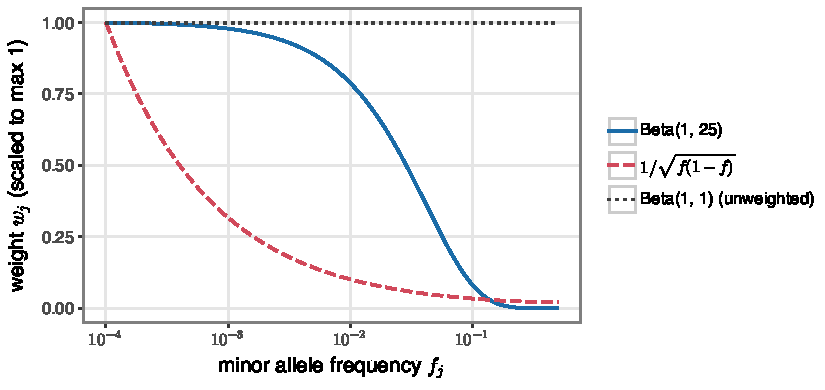
\includegraphics[width=0.8\linewidth]{maf_weights.pdf}
  \caption{Variant weights as a function of MAF, each scaled to a maximum of one: the $\BetaD(1,25)$ density used by default in SKAT, the Madsen-Browning weight $1/\sqrt{f(1-f)}$, and equal weights.}
  \label{fig:maf_weights}
\end{figure}

\subsection{SKAT-O}

We rarely know in advance whether a gene's variants act in one direction. SKAT-O~\citep{lee2012} computes $Q_\rho$ over a grid $0=\rho_1<\rho_2<\dots<\rho_B=1$, for example $\rho\in\{0,0.1^2,0.2^2,0.3^2,0.4^2,0.5^2,1\}$, and uses the smallest p-value,
\begin{equation}
  T = \min_{b=1,\dots,B} p_{\rho_b},
\end{equation}
where $p_{\rho_b}$ is the p-value of $Q_{\rho_b}$. $T$ is not itself a p-value, because taking the minimum over several tests makes small values more likely. Its null distribution follows from the joint distribution of the $Q_\rho$, which are all quadratic forms in the same $\vS$. Because $Q_\rho$ is linear in $\rho$, it is a combination of $Q_{\text{SKAT}}$ and $Q_{\text{burden}}$, and \citet{lee2012} decompose it into a $\chi^2_1$ part and an approximately independent remainder, which reduces the p-value of $T$ to a one-dimensional numerical integral. They also give a small-sample correction for binary traits, where the asymptotic null distribution can be poor.

Why not estimate $\rho$, for example by maximum likelihood, and plug it in? Under $H_0$, $\tau=0$ and $\rho$ has no effect on the likelihood: it is not identifiable. A parameter that exists only under the alternative breaks the usual asymptotic theory for likelihood ratio and score tests, so the plug-in statistic has no standard null distribution. Taking the minimum p-value over a grid and computing the exact null distribution of the minimum sidesteps the problem. The price is a modest loss of power relative to knowing the best $\rho$ in advance.

\subsection{Comparing the tests}

Figure~\ref{fig:skat_power} compares the three tests in a simulated region of 39 rare variants. When most variants are causal and all increase the trait, the burden test is the most powerful. When few variants are causal, or when effects have mixed signs, SKAT is much more powerful, and with mixed signs the burden test has almost no power at all. SKAT-O is close to the better of the two in every setting. It is never the best by much, but it is never far from the best, which is why it is a common default.

\begin{figure}[!htbp]
  \centering
  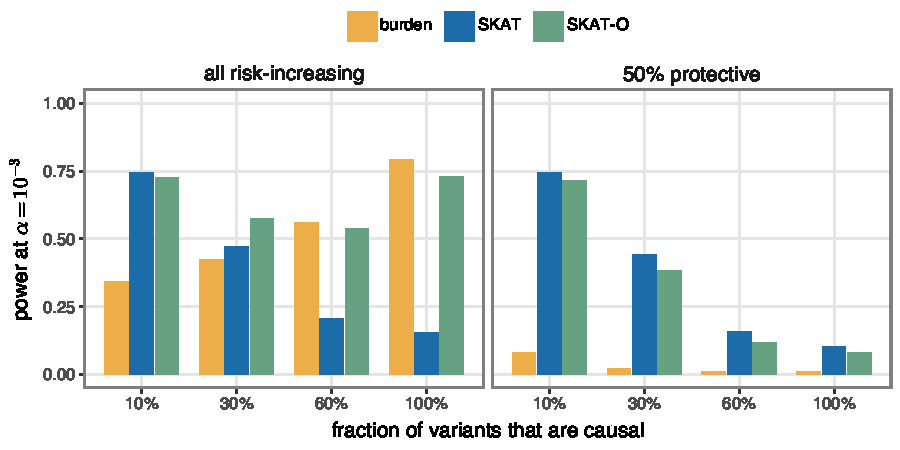
\includegraphics[width=0.9\linewidth]{skat_power.pdf}
  \caption{Power of burden, SKAT and SKAT-O tests (with $\BetaD(1,25)$ weights) in a simulated region of $M=39$ independent variants with MAF between 0.0005 and 0.02, for a quantitative trait in $N=2000$ individuals. Each variant is causal with the probability on the horizontal axis and has effect $|\beta_j|=a|\log_{10}f_j|$, with the sign either always positive (left) or random (right). The scale $a$ is smaller for larger causal fractions, so power should be compared between tests within a group of bars, not across groups. Null distributions were computed by simulating $2\times10^5$ score vectors for the fixed genotype matrix; 1000 replicates per setting.}
  \label{fig:skat_power}
\end{figure}

%======================================================================
\section{Using functional annotations in the test}
\label{sec:fst}
%======================================================================

A pathogenicity score such as LINSIGHT, CADD or Eigen gives, for each variant, an estimate of how likely it is to be functional. There are two simple ways to use it in a set-based test: filter variants on a threshold, as in a burden analysis, or multiply the MAF weights by the score, $w_j\to w_jZ_j$, where $Z_j\geq 0$ is the score of variant $j$. Both help if the score predicts which variants affect the trait and hurt if it does not. For noncoding variants, where scores are weak and a score built for one purpose (say, conservation) may not predict effects on a particular trait, this matters. \citet{he2017} proposed tests that use several annotations at once and lose little power when an annotation is uninformative. We call this the functional score test (FST).

\subsection{The model}

Let $q$ be the number of annotations and $Z_{jk}$ the $k$-th functional score of variant $j$, $k=1,\dots,q$. The effect of variant $j$ is decomposed as
\begin{equation}
  \beta_j = \gamma_{j0} + \sum_{k=1}^q Z_{jk}\gamma_{jk} ,
\end{equation}
where each $\gamma_{jk}$ is random with mean zero, $\Var(\gamma_{jk})=w_j^2\tau_k$ and $\Cov(\gamma_{j_1k},\gamma_{j_2k})=\rho\,w_{j_1}w_{j_2}\tau_k$, and the $\gamma_{j0},\dots,\gamma_{jq}$ are independent for each $j$. The variance component $\tau_k\geq 0$ measures how much of the genetic effect in the region tracks annotation $k$, and $\tau_0$ the part that tracks no annotation. Then
\begin{align}
  \Var(\beta_j) &= w_j^2\Big(\tau_0+\sum_{k=1}^q Z_{jk}^2\tau_k\Big), \\
  \Cov(\beta_{j_1},\beta_{j_2}) &= \rho\,w_{j_1}w_{j_2}\Big(\tau_0+\sum_{k=1}^q Z_{j_1k}Z_{j_2k}\tau_k\Big).
\end{align}
Setting $Z_{j0}=1$ and $\mD_k=\operatorname{diag}(w_1Z_{1k},\dots,w_MZ_{Mk})$, the covariance of $\vb$ is a sum of SKAT-O covariances, one per annotation,
\begin{equation}
  \Cov(\vb) = \sum_{k=0}^q \tau_k\,\mD_k\mR_\rho\mD_k ,
\end{equation}
and the null hypothesis of no association is $H_0:\tau_0=\tau_1=\dots=\tau_q=0$.

\subsection{The test}

Repeating the derivation of Section~\ref{sec:skat} for each $\tau_k$ in turn gives one score statistic per annotation,
\begin{equation}
  Q_{\rho,k} = \vS^\top\mD_k\mR_\rho\mD_k\vS = (1-\rho)\sum_{j=1}^M w_j^2Z_{jk}^2S_j^2 + \rho\Big(\sum_{j=1}^M w_jZ_{jk}S_j\Big)^2 ,
\end{equation}
which is the SKAT-O statistic with weights $w_jZ_{jk}$. $Q_{\rho,0}$ is the original test with MAF weights only. \citet{he2017} combine these statistics by their minimum p-value, $T=\min_{k,\rho}p_{\rho,k}$, over $k=0,\dots,q$ and, in practice, $\rho\in\{0,1\}$, so that the combined test takes the best of the dispersion and burden tests for each annotation. The null distribution of $T$ is obtained from the null distribution of $\vS$ alone. Score vectors are drawn from $\Normal(\mathbf{0},\hat\sigma^2\boldsymbol{\Omega})$, each $p_{\rho,k}$ is computed by moment matching, and the vector of normal scores $\boldsymbol\delta$ with elements $\Phi^{-1}(p_{\rho,k})$ is approximated as multivariate normal with the correlation matrix estimated from the draws. The p-value of an observed $T=t$ is then $1-P(\delta_{\rho,k}>\Phi^{-1}(t)\text{ for all }k,\rho)$, a multivariate normal probability. Only $\vS$ and $\boldsymbol{\Omega}$ are needed, so the test works with summary statistics and, by adding them across studies, in meta-analysis.

The construction has a simple logic. The unified test always contains the original test, $k=0$, so when the annotations are uninformative it loses only what the multiple-testing correction across the $2(q+1)$ statistics costs. When an annotation is informative, the corresponding reweighted statistic carries the signal.

\subsection{Power}

\citet{he2017} simulated regions in which 10\% of variants were causal and annotation $k$ predicted the causal variants with probability $P_k$. They compared the original tests with $\BetaD(1,25)$ weights (O), tests with weights multiplied by the first score (W1), and unified tests with the first score (U1) or the first two scores (U1+2). When neither score was informative ($P_1=P_2=0$), W1 lost a large fraction of the power of O while U1 and U1+2 lost none, and could even gain slightly. When the first score was informative, W1, U1 and U1+2 all improved on O. When only the second score was informative, U1+2 was the most powerful and W1 the least. The pattern held for dispersion, burden and combined tests.

Figure~\ref{fig:fst_power} reproduces the logic in a small simulation of our own, using a region simulated as in Figure~\ref{fig:skat_power} and a single annotation. With an uninformative score, reweighting (W) costs most of the power, while the unified test (U) stays close to the original (O). With an informative score, reweighting helps the burden test a great deal, because it removes the neutral variants that dilute the burden, and the unified test captures most of the gain. SKAT gains less from the annotation, since squaring the scores already lets the variants with large $S_j$ dominate.

\begin{figure}[!htbp]
  \centering
  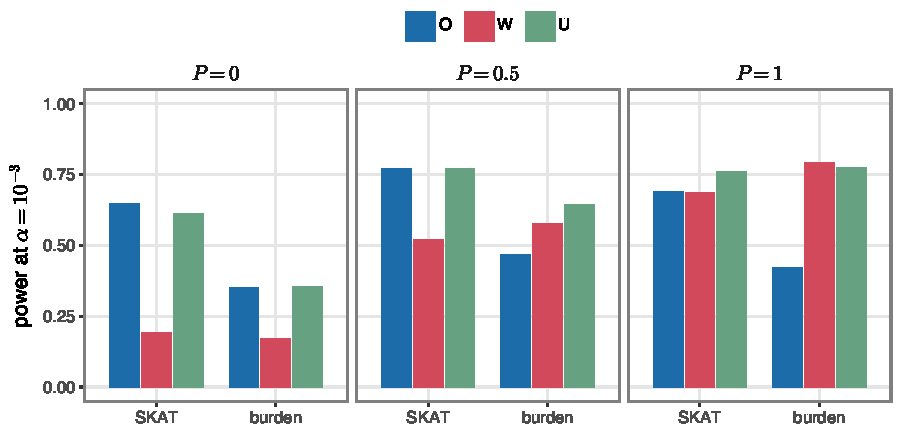
\includegraphics[width=0.9\linewidth]{fst_power.pdf}
  \caption{Power of SKAT and burden tests with $\BetaD(1,25)$ weights (O), weights multiplied by a functional score (W), and the unified minimum p-value test over both weightings (U). In a region simulated as in Figure~\ref{fig:skat_power}, 20\% of variants are causal with positive effects $\beta_j=0.28|\log_{10}f_j|$. The score is $\chi^2_1$ for non-causal variants; for each causal variant it is non-central $\chi^2_1$ (non-centrality 4) with probability $P$ and $\chi^2_1$ otherwise. 50 draws of the causal set and scores, 20 trait replicates each, $\alpha=10^{-3}$. Within a panel the tests are applied to the same simulated traits.}
  \label{fig:fst_power}
\end{figure}

%======================================================================
\section{Case study: noncoding de novo mutations in autism}
\label{sec:autism}
%======================================================================

Autism spectrum disorder (ASD) has a substantial contribution from de novo mutations. Exome sequencing of families found that children with ASD carry more de novo protein-truncating mutations than their unaffected siblings~\citep{iossifov2014}, and burden tests of such mutations have identified many ASD genes. In Chapter 10 we saw that de novo mutations predicted by SpliceAI to disrupt splicing are also enriched in ASD and intellectual disability. Most de novo mutations, about 70 per genome, fall outside coding sequence, and whether noncoding de novo mutations contribute was an open question. Noncoding mutations cannot be tested one at a time, and there is no simple equivalent of ``protein-truncating'' to define which ones to aggregate. \citet{zhou2019} used deep learning sequence models to supply that definition.

\subsection{Data and design}

The data were whole genomes from 1,790 \emph{simplex} families from the Simons Simplex Collection, 7,097 genomes in total. A simplex family has exactly one affected child, the proband, together with unaffected parents and, in most families, an unaffected sibling (Figure~\ref{fig:asd_pipeline}). Simplex families are enriched for de novo causes, because an inherited cause of large effect would often have affected other family members. The unaffected siblings are a natural control group. They have the same parents, so their expected de novo mutation rate is similar, and their genomes were sequenced and processed in the same way as the probands', so technical artefacts in mutation calling affect both groups alike. The comparison is therefore between the de novo mutations of probands and those of siblings, and the question is whether the probands' mutations are more damaging.

\subsection{Scoring mutations}

Each de novo mutation was scored with two DeepSEA-style convolutional networks (Chapter 2), which take 1,000 bp of sequence centred on the variant and predict the probability of each of many chromatin or RNA-binding features. The transcriptional regulation model predicts 2,002 features (DNase hypersensitivity, transcription factor binding and histone marks) and was trained on ENCODE and Roadmap Epigenomics profiles. The post-transcriptional model predicts 232 features, mostly RNA-binding protein (RBP) binding sites measured by CLIP-seq, which captures the sites on RNA bound by a given protein. For each mutation and feature $\ell$, the variant effect is the absolute difference between the predictions for the two alleles, $|p_\ell(\text{alt})-p_\ell(\text{ref})|$.

These thousands of predicted effects must be reduced to one number per mutation, the probability that it is harmful. \citet{zhou2019} trained a regularized logistic regression (Chapter 1) with the standardized predicted effects as features, separately for transcriptional and post-transcriptional effects. Positive examples were 4,401 noncoding regulatory mutations reported in HGMD to cause disease. Negative examples were 999,668 \emph{singleton} variants observed in healthy individuals in the 1000 Genomes Project. Singletons are a better negative set than common variants because they are rare, like de novo mutations, and so have similar sequence context and mutational processes; they are mostly benign, but selection has had little time to remove the damaging ones, so the negative set is somewhat contaminated. Classes were weighted inversely to their size to counter the imbalance. The predicted probabilities were standardized across all proband and sibling mutations to give a \emph{disease impact score} (DIS) for each mutation. The classifier never sees autism data: it learns what Mendelian disease mutations look like through the eyes of the sequence models, and is then applied to a different disease.

\begin{figure}[!htbp]
  \centering
  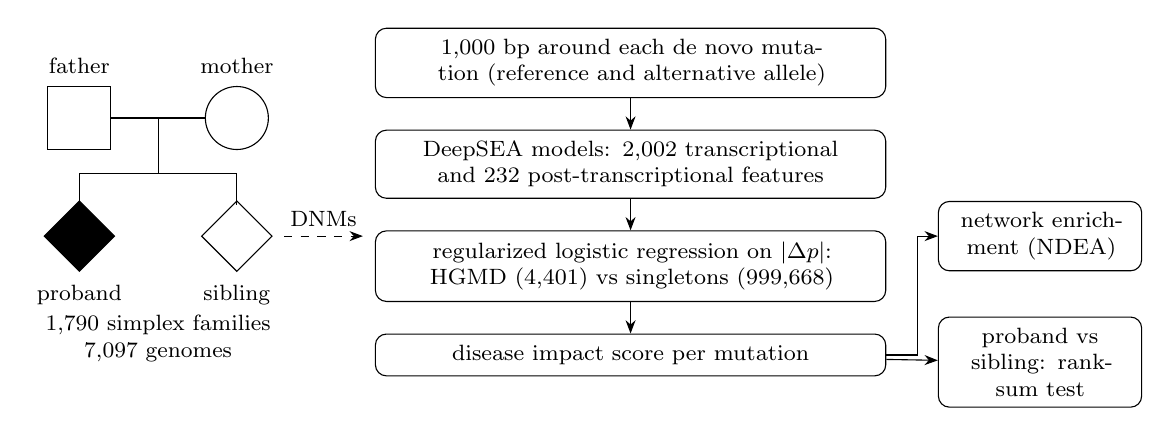
\begin{tikzpicture}[>=Stealth, every node/.style={font=\small},
      box/.style={draw, rounded corners, align=center, inner sep=4pt}]
    % pedigree
    \node[draw, minimum size=8mm] (fa) at (0,2.2) {};
    \node[draw, circle, minimum size=8mm] (mo) at (2.0,2.2) {};
    \node[above=1pt of fa, font=\footnotesize] {father};
    \node[above=1pt of mo, font=\footnotesize] {mother};
    \draw (fa.east) -- (mo.west);
    \draw (1.0,2.2) -- (1.0,1.5) -- (0,1.5) -- (0,1.1);
    \draw (1.0,1.5) -- (2.0,1.5) -- (2.0,1.1);
    \node[draw, diamond, fill=black, minimum size=9mm, inner sep=0pt] (pr) at (0,0.7) {};
    \node[draw, diamond, minimum size=9mm, inner sep=0pt] (sb) at (2.0,0.7) {};
    \node[below=1pt of pr, font=\footnotesize] {proband};
    \node[below=1pt of sb, font=\footnotesize] {sibling};
    \node[align=center, font=\footnotesize] at (1.0,-0.6) {1,790 simplex families\\7,097 genomes};
    % pipeline
    \begin{scope}[box/.append style={text width=6.2cm, font=\footnotesize}]
    \node[box] (seq) at (7.0,2.9) {1,000 bp around each de novo mutation (reference and alternative allele)};
    \node[box, below=4mm of seq] (cnn) {DeepSEA models: 2,002 transcriptional and 232 post-transcriptional features};
    \node[box, below=4mm of cnn] (lr) {regularized logistic regression on $|\Delta p|$: HGMD (4,401) vs singletons (999,668)};
    \node[box, below=4mm of lr] (dis) {disease impact score per mutation};
    \end{scope}
    \node[box, text width=2.3cm, font=\footnotesize] (cmp) at (12.2,-0.9) {proband vs sibling: rank-sum test};
    \node[box, text width=2.3cm, font=\footnotesize] (nd) at (12.2,0.7) {network enrichment (NDEA)};
    \draw[->] (seq) -- (cnn); \draw[->] (cnn) -- (lr); \draw[->] (lr) -- (dis);
    \draw[->] (dis) -- (cmp); \draw[->] (dis.east) -- ++(0.4,0) |- (nd.west);
    \draw[->, dashed] (2.6,0.7) -- (3.6,0.7) node[midway, above, font=\footnotesize] {DNMs};
  \end{tikzpicture}
  \caption{Design of the autism noncoding mutation study. Each simplex family has one affected child (proband, filled) and an unaffected sibling. De novo mutations (DNMs) are scored by sequence models, the predicted effects are combined into a disease impact score by a classifier trained on known disease mutations, and the scores of proband and sibling mutations are compared. After \citet{zhou2019}.}
  \label{fig:asd_pipeline}
\end{figure}

\subsection{Comparing probands and siblings}

The scores of proband and sibling mutations were compared with a one-sided Wilcoxon rank-sum (Mann-Whitney) test. Let $d^P_1,\dots,d^P_{n_P}$ be the DIS values of proband mutations and $d^S_1,\dots,d^S_{n_S}$ those of sibling mutations. Rank all $n_P+n_S$ values together, let $R_P$ be the sum of the ranks of the proband mutations, and define $U=R_P-n_P(n_P+1)/2$, the number of (proband, sibling) pairs in which the proband mutation has the higher score. Under the null hypothesis that the two groups have the same distribution, and with no ties,
\begin{equation}
  \E[U]=\frac{n_Pn_S}{2}, \qquad \Var(U)=\frac{n_Pn_S(n_P+n_S+1)}{12},
\end{equation}
and $(U-\E[U])/\sqrt{\Var(U)}$ is approximately standard normal for large samples. The test uses only ranks, so it is robust to the heavy tail of the score distribution, in which a few mutations have very high predicted impact. The quantity $U/(n_Pn_S)$ is the probability that a random proband mutation scores higher than a random sibling mutation, the same quantity as the AUROC of Chapter 1.

Proband mutations had significantly higher disease impact scores than sibling mutations, for both transcriptional and post-transcriptional effects (Figure~\ref{fig:asd_dis}). The difference was larger for mutations near genes, and larger again near genes that are intolerant of loss-of-function variation in the population. The effect is small on average, as expected if only a minority of probands carry a causal noncoding mutation.

\begin{figure}[!htbp]
  \centering
  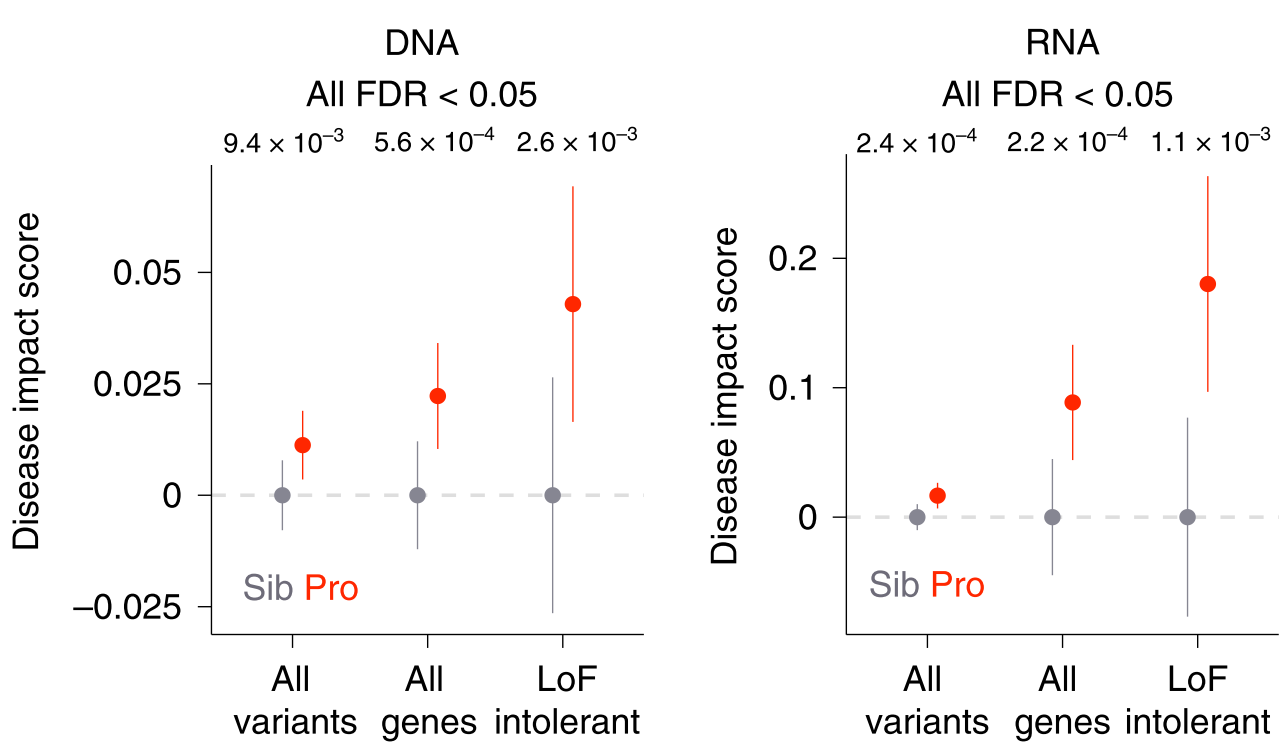
\includegraphics[width=0.7\linewidth]{slides/asd_disease_impact.png}
  \caption{Mean disease impact score of de novo mutations in probands (red) and unaffected siblings (grey), for predicted transcriptional (DNA) and post-transcriptional (RNA) effects. Scores are normalized by subtracting the sibling mean, so siblings are at zero; bars show 95\% confidence intervals. Mutations are shown for all variants, variants assigned to any gene, and variants assigned to genes intolerant of loss of function, with the significance of each comparison above; all comparisons have false discovery rate below 0.05. Reproduced from \citet{zhou2019}.}
  \label{fig:asd_dis}
\end{figure}

%======================================================================
\section{Network differential enrichment analysis}
\label{sec:ndea}
%======================================================================

Even with a good score, de novo mutations are too sparse to implicate individual genes: most genes receive no mutation in either group, and few receive more than one. \citet{zhou2019} therefore borrowed strength across genes using a gene network. The network was the brain-specific functional network of \citet{greene2015}, one of a set of tissue-specific networks built by Bayesian integration of thousands of genome-scale data sets (expression, protein interactions, and others) against tissue-specific gold standards. Unlike the co-expression and partial-correlation networks of Chapter 9, its edges are not estimated from one data type: the weight $A_{uv}\in[0,1]$ is the posterior probability that genes $u$ and $v$ act together in brain.

Network differential enrichment analysis (NDEA) asks, for each gene $u$, whether the mutations in genes functionally connected to $u$ have higher scores in probands than in siblings. Let $\mathcal{P}$ and $\mathcal{S}$ be the sets of proband and sibling mutations, $d_m$ the disease impact score of mutation $m$, and $v(m)$ the gene to which it is assigned (the nearest gene within a distance threshold). Each mutation receives a weight for gene $u$,
\begin{equation}
  a_{um} = \frac{A_{u,v(m)}}{n_{v(m)}} ,
\end{equation}
where $n_{v}$ is the number of mutations in the same group (proband or sibling) assigned to gene $v$, so that a gene with many mutations does not dominate. The weighted mean scores of the two groups are
\begin{equation}
  \mu_{\mathcal{P}}(u) = \frac{\sum_{m\in\mathcal{P}}a_{um}d_m}{\sum_{m\in\mathcal{P}}a_{um}}, \qquad
  \mu_{\mathcal{S}}(u) = \frac{\sum_{m\in\mathcal{S}}a_{um}d_m}{\sum_{m\in\mathcal{S}}a_{um}} ,
\end{equation}
and they are compared with a weighted version of Welch's $t$ statistic,
\begin{equation}
  t_u = \frac{\mu_{\mathcal{P}}(u)-\mu_{\mathcal{S}}(u)}{\sqrt{V_{\mathcal{P}}(u)/N_{\mathcal{P}}(u)+V_{\mathcal{S}}(u)/N_{\mathcal{S}}(u)}} .
  \label{eq:ndea}
\end{equation}
Here, for group $\mathcal{G}\in\{\mathcal{P},\mathcal{S}\}$, dropping the dependence on $u$,
\begin{equation}
  V_{\mathcal{G}} = \frac{\sum_{m\in\mathcal{G}}a_{m}(d_m-\mu_{\mathcal{G}})^2}{\sum_{m\in\mathcal{G}}a_m-\sum_{m\in\mathcal{G}}a_m^2\big/\sum_{m\in\mathcal{G}}a_m}, \qquad
  N_{\mathcal{G}} = \frac{\left(\sum_{m\in\mathcal{G}}a_m\right)^2}{\sum_{m\in\mathcal{G}}a_m^2} .
\end{equation}
Both quantities generalize their unweighted counterparts. Suppose the $d_m$ in a group are independent with mean $\mu$ and variance $v$, and the weights are fixed. Writing $A_1=\sum_m a_m$ and $A_2=\sum_m a_m^2$, the weighted mean $\hat\mu=\sum_m a_md_m/A_1$ has variance
\begin{equation}
  \Var(\hat\mu) = \frac{\sum_m a_m^2 v}{A_1^2} = \frac{v}{N}, \qquad N=\frac{A_1^2}{A_2},
\end{equation}
so $N$ is the \emph{effective sample size}: the number of equally weighted observations that would give the same variance. It equals the number of mutations when the weights are equal, and is smaller when a few mutations carry most of the weight. For the variance, $\sum_ma_m(d_m-\hat\mu)^2=\sum_ma_md_m^2-A_1\hat\mu^2$, with $\E[\sum_ma_md_m^2]=A_1(v+\mu^2)$ and $\E[\hat\mu^2]=\mu^2+vA_2/A_1^2$, so
\begin{equation}
  \E\Big[\sum_ma_m(d_m-\hat\mu)^2\Big] = A_1(v+\mu^2) - A_1\mu^2 - v\frac{A_2}{A_1} = v\left(A_1-\frac{A_2}{A_1}\right),
\end{equation}
and $V$ is an unbiased estimate of $v$. With equal weights $a_m=1$ in a group of $n$ mutations, $A_1=n$, $A_2=n$, $N=n$ and $V=\sum_m(d_m-\hat\mu)^2/(n-1)$, the usual sample variance, so~\eqref{eq:ndea} reduces to Welch's $t$. The statistic is compared with a $t$ distribution whose degrees of freedom follow from the Welch-Satterthwaite approximation with $N_{\mathcal{P}}$ and $N_{\mathcal{S}}$ in place of the group sizes.

A gene can score highly without carrying a single mutation, if its network neighbours carry high-impact proband mutations (Figure~\ref{fig:ndea}). The same test applies to a gene set, such as a Gene Ontology (GO) term, by treating the set as one node whose edge weight to gene $v$ is the average of $A_{u v}$ over the genes $u$ in the set. Among the terms enriched at false discovery rate below 0.05 were many neuronal functions: regulation of synapse assembly, axon guidance, dendrite development, the synaptic vesicle cycle, postsynaptic density and neuron migration. Clustering the top-ranked genes on the network gave groups related to synaptic function and to chromatin regulation. Both themes had already emerged from coding de novo mutations in ASD: genes for synaptic function, which are specific to neurons, and genes for transcriptional and chromatin regulation, which act in every cell type yet seem to matter most for neurodevelopment. The noncoding mutations point to the same biology.

\begin{figure}[!htbp]
  \centering
  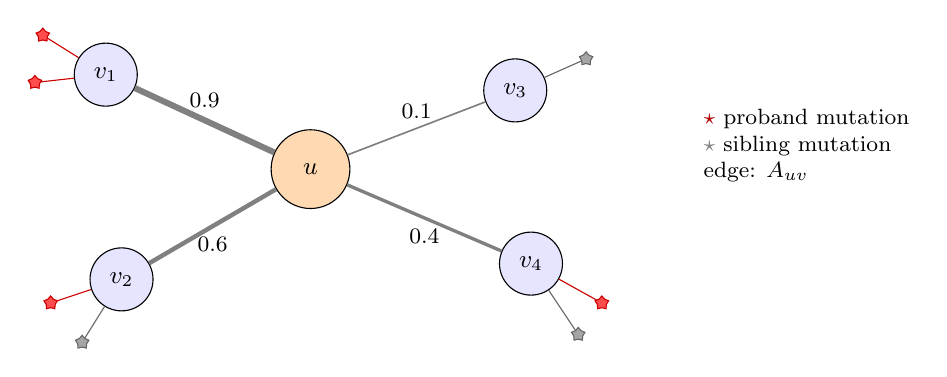
\begin{tikzpicture}[>=Stealth, every node/.style={font=\small},
      gene/.style={circle, draw, minimum size=8mm, inner sep=0pt, fill=blue!10}]
    \node[gene, fill=orange!30, minimum size=10mm] (u) at (0,0) {$u$};
    \node[gene] (v1) at (-2.6,1.2) {$v_1$};
    \node[gene] (v2) at (-2.4,-1.4) {$v_2$};
    \node[gene] (v3) at (2.6,1.0) {$v_3$};
    \node[gene] (v4) at (2.8,-1.2) {$v_4$};
    \draw[line width=2.2pt, gray] (u) -- node[above, black, font=\footnotesize] {0.9} (v1);
    \draw[line width=1.6pt, gray] (u) -- node[below, black, font=\footnotesize] {0.6} (v2);
    \draw[line width=0.6pt, gray] (u) -- node[above, black, font=\footnotesize] {0.1} (v3);
    \draw[line width=1.2pt, gray] (u) -- node[below, black, font=\footnotesize] {0.4} (v4);
    \foreach \n/\c/\dx/\dy in {v1/red/-0.8/0.5, v1/red/-0.9/-0.1, v2/red/-0.9/-0.3, v2/gray/-0.5/-0.8, v3/gray/0.9/0.4, v4/red/0.9/-0.5, v4/gray/0.6/-0.9} {
      \draw[\c!80!black] (\n) -- ++(\dx,\dy) node[star, star points=5, fill=\c!70, draw=\c!80!black, inner sep=1.2pt] {};
    }
    \node[align=left, font=\footnotesize] at (6.3,0.3) {\textcolor{red!70!black}{$\star$} proband mutation\\\textcolor{gray}{$\star$} sibling mutation\\edge: $A_{uv}$};
  \end{tikzpicture}
  \caption{Network differential enrichment analysis for gene $u$. Mutations assigned to other genes $v$ are weighted by the network edge weight $A_{uv}$, and the weighted mean disease impact scores of proband and sibling mutations are compared with a weighted $t$ test. Gene $u$ can be implicated without carrying a mutation itself.}
  \label{fig:ndea}
\end{figure}

%======================================================================
\section{Experimental validation}
\label{sec:validation}
%======================================================================

Statistical enrichment shows that proband mutations as a group have higher predicted impact, not that any particular mutation does anything. \citet{zhou2019} tested prioritized mutations with \emph{luciferase reporter assays}. For each selected proband mutation with predicted transcriptional effect (positive disease impact score, near a gene with prior evidence for a role in ASD), 230 bp of sequence around the mutation was cloned, once with the de novo allele and once with the reference allele carried by the sibling, upstream of a minimal promoter driving the firefly luciferase gene. The constructs were transfected into a human neuroblastoma cell line, and the light produced, normalized to a co-transfected control reporter and to the empty vector, measures how strongly each sequence drives transcription. Of 59 tested regions that showed transcriptional activity, 57 showed a significant difference between the two alleles (Figure~\ref{fig:luciferase}). A predicted splicing-disrupting mutation was tested in a similar way with a minigene, a reporter containing the exon and flanking introns, and reduced inclusion of the exon.

\begin{figure}[!htbp]
  \centering
  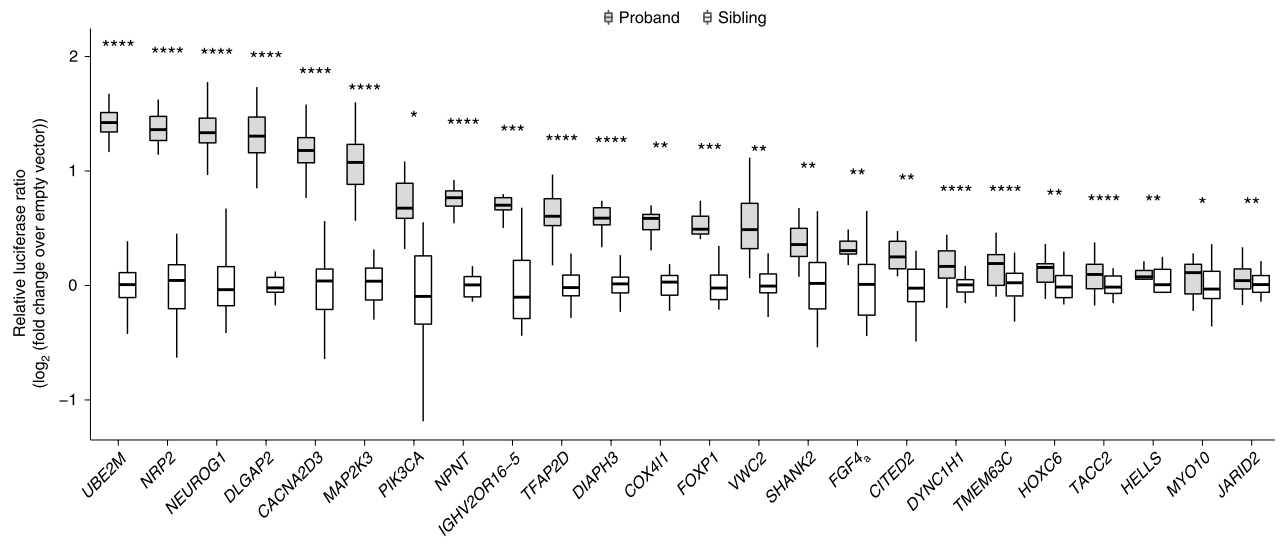
\includegraphics[width=\linewidth]{slides/asd_luciferase.png}
  \caption{Luciferase reporter activity (log$_2$ fold change over empty vector) of sequences carrying the proband's de novo allele (grey) or the reference allele carried by the sibling (white), for prioritized mutations near the genes shown. Asterisks mark significant differences between alleles. Reproduced from \citet{zhou2019}.}
  \label{fig:luciferase}
\end{figure}

Reporter assays have clear limits. The sequence is tested outside its chromosomal context, on a plasmid, in one cell line that may not express the relevant transcription factors, and without the gene it normally regulates. A difference between alleles shows that the mutation changes regulatory activity, not that the change affects the target gene in the developing brain, let alone that it contributes to ASD. Massively parallel reporter assays apply the same idea to thousands of sequences at once, and genome editing of the endogenous locus gives stronger evidence at much greater cost.

%======================================================================
\section{Using molecular data from patients}
\label{sec:molecular}
%======================================================================

So far the evidence that a rare variant matters has come from prediction or from aggregating many individuals. For a patient with a suspected Mendelian disease, the question is narrower: which of the patient's rare variants, if any, causes the disease? Exome or genome sequencing finds a causal variant in only a minority of patients, often because the culprit is noncoding or its effect is not recognizable from sequence. RNA-seq from the patient, increasingly obtained alongside whole-genome sequencing in clinical genetics, can show the consequence of a variant directly. A variant that disrupts a promoter or enhancer lowers the expression of the haplotype that carries it (Figure~\ref{fig:reg_variant}); one that disrupts a splice site produces aberrant isoforms; one that creates a premature stop codon triggers nonsense-mediated decay of the transcript. Each leaves a trace in RNA-seq, and the task is to recognize a trace that is unusual relative to the population. The tissue matters: the relevant gene must be expressed in the sample, which is why blood, skin fibroblasts and, for muscle diseases, muscle biopsies are used.

\begin{figure}[!htbp]
  \centering
  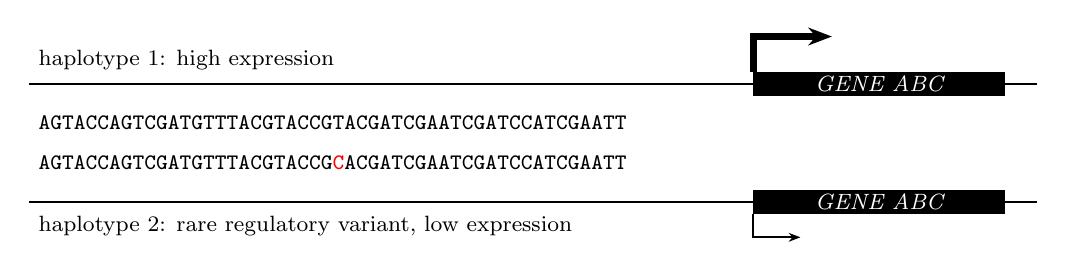
\begin{tikzpicture}[>=Stealth, every node/.style={font=\small}]
    \node[font=\ttfamily\footnotesize, anchor=west] (s1) at (0,0.25) {AGTACCAGTCGATGTTTACGTACCGTACGATCGAATCGATCCATCGAATT};
    \node[font=\ttfamily\footnotesize, anchor=west] (s2) at (0,-0.25) {AGTACCAGTCGATGTTTACGTACCG\textcolor{red}{C}ACGATCGAATCGATCCATCGAATT};
    \draw[thick] (0,0.75) -- (12.8,0.75);
    \draw[thick] (0,-0.75) -- (12.8,-0.75);
    \fill (9.2,0.6) rectangle (12.4,0.9); \node[white, font=\footnotesize\itshape] at (10.8,0.75) {GENE ABC};
    \fill (9.2,-0.9) rectangle (12.4,-0.6); \node[white, font=\footnotesize\itshape] at (10.8,-0.75) {GENE ABC};
    \draw[line width=2.5pt, -{Stealth[length=3mm]}] (9.2,0.9) -- (9.2,1.35) -- (10.2,1.35);
    \draw[line width=0.6pt, -{Stealth[length=1.5mm]}] (9.2,-0.9) -- (9.2,-1.2) -- (9.8,-1.2);
    \node[right, font=\footnotesize] at (0,1.05) {haplotype 1: high expression};
    \node[right, font=\footnotesize] at (0,-1.05) {haplotype 2: rare regulatory variant, low expression};
  \end{tikzpicture}
  \caption{A rare variant (red) in a regulatory element upstream of a gene reduces transcription from the haplotype that carries it. In RNA-seq this appears as reduced total expression and as allelic imbalance at heterozygous sites in the gene.}
  \label{fig:reg_variant}
\end{figure}

\subsection{Expression and splicing outliers}

An \emph{expression outlier} is a gene whose expression in the patient is extreme relative to a reference population, such as the GTEx samples of the same tissue. After normalizing expression and removing the effects of known covariates and hidden confounders (Chapter 12), the expression of gene $u$ in the patient is converted to a $z$-score, $z_u=(e_u-\bar e_u)/s_u$, with $\bar e_u$ and $s_u$ the mean and standard deviation of the normalized expression $e_u$ across the reference samples (Figure~\ref{fig:outliers}a). In GTEx, individuals who were expression outliers for a gene, particularly consistently across tissues, were enriched for rare variants near that gene, with the strongest enrichment for structural variants, frameshifts and splice-site variants~\citep{li2017}. Combining expression, splicing and allelic outlier signals with variant annotations improves the prioritization further~\citep{ferraro2020}.

A \emph{splicing outlier} is an aberrant splicing event: a splice junction that is used in the patient but rarely or never in controls, or a change in the relative usage of junctions (Figure~\ref{fig:outliers}b). Splicing quantification was the subject of Chapter 10. \citet{cummings2017} applied RNA-seq of muscle biopsies to patients with rare muscle disorders who remained undiagnosed after exome or genome sequencing, and found pathogenic exon skipping, exon extension and splice-site creation events absent from GTEx muscle samples, which established a diagnosis for a substantial fraction of the patients. Several of the causal variants were deep intronic or exonic changes whose effect on splicing had not been recognized from sequence.

\begin{figure}[!htbp]
  \centering
  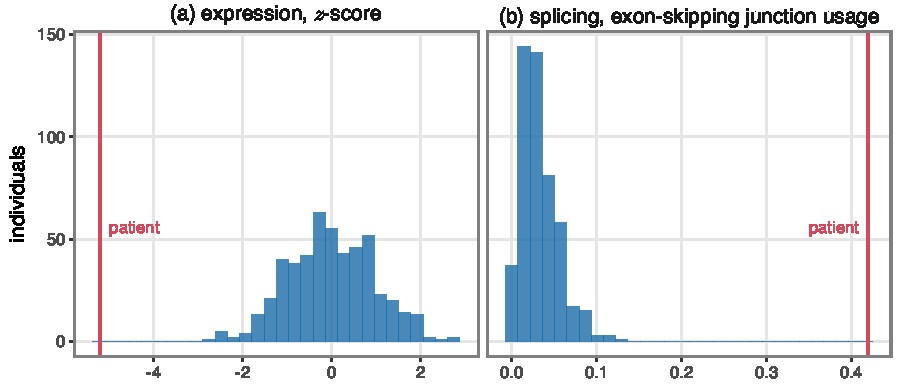
\includegraphics[width=0.95\linewidth]{outliers.pdf}
  \caption{Outlier detection against a reference population of 500 simulated individuals. (a) Expression $z$-scores of one gene; the patient (red) has $z=-5.2$. (b) Fraction of reads at an exon that use a junction skipping it; the patient uses the skipping junction in 42\% of reads, against a few percent in the reference population.}
  \label{fig:outliers}
\end{figure}

\subsection{Allelic outliers}

Allele-specific expression (ASE), introduced in Chapter 12, gives a test within the patient: at a heterozygous site in a transcribed region, the reads from the two haplotypes can be counted, and an imbalance means that one haplotype is expressed more than the other. A rare regulatory variant or a nonsense-mediated decay trigger on one haplotype produces exactly this. The difficulty is that allelic imbalance is common. Most genes have common eQTLs, and in any individual, the two haplotypes of a gene often differ in expression for reasons unrelated to disease. A raw test of imbalance against $1/2$ flags thousands of genes per person.

ANEVA-DOT~\citep{mohammadi2019} addresses this by asking whether the imbalance is unusual \emph{for that gene}. Genes differ in how much regulatory variation the population tolerates. For a dosage-sensitive gene, selection keeps regulatory variants rare and their effects small, so the genetic variance of its expression is low; for a tolerant gene, large common eQTL effects are normal. ANEVA estimates this genetic variance, $V^G$, for each gene from ASE data in a reference population (GTEx). ANEVA-DOT then tests a patient's allelic counts against the distribution implied by $V^G$.

A simplified version of the model is as follows. Let $s\in\R$ be the log$_2$ ratio of the expression of haplotype 1 to haplotype 2 in an individual, the allelic fold change. In the population, $s\sim\Normal(0,V^G)$. Given $s$, a read comes from haplotype 1 with probability $\pi(s)=2^s/(1+2^s)$, and with $n$ reads at the site, the count $r$ from haplotype 1 is beta-binomial (Chapter 12), which allows for overdispersion from technical sources such as PCR duplicates,
\begin{equation}
  r\mid s \sim \operatorname{BetaBinomial}\big(n,\ c\,\pi(s),\ c\,(1-\pi(s))\big),
\end{equation}
where $c>0$ is a concentration parameter. Integrating over $s$ gives the null distribution of $r$ for a patient whose regulatory variation is typical of the population,
\begin{equation}
  P(r\mid n) = \int \Normal(s\mid 0, V^G)\,P(r\mid n,s)\,ds ,
\end{equation}
and the two-sided p-value of the observed count $r_{\text{obs}}$ is $2\min\{P(r\leq r_{\text{obs}}\mid n),P(r\geq r_{\text{obs}}\mid n)\}$. Figure~\ref{fig:aneva_dot} shows the same patient counts, 640 reads from one haplotype and 157 from the other, a four-fold imbalance, against two genes. For a gene with low $V^G$ the imbalance is far outside the population distribution ($p\approx 10^{-12}$); for a gene with high $V^G$ it is unremarkable ($p\approx 0.07$). The scale of what counts as an outlier is set by the population, gene by gene.

\begin{figure}[!htbp]
  \centering
  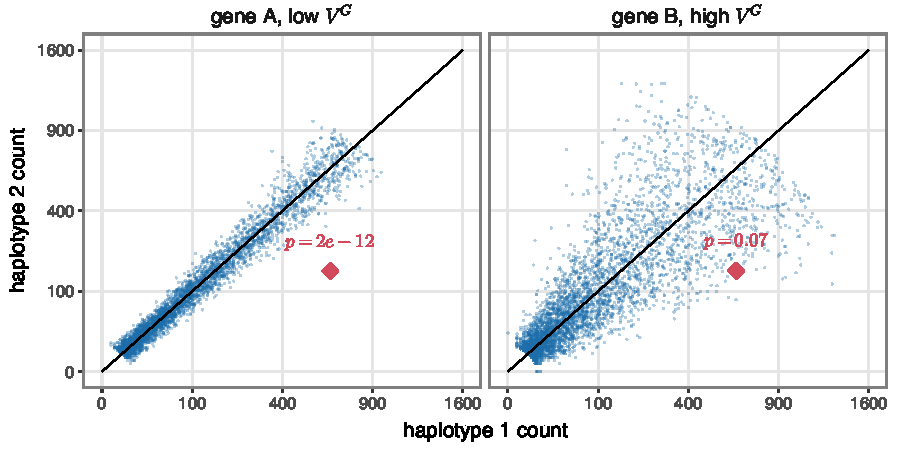
\includegraphics[width=0.9\linewidth]{aneva_dot.pdf}
  \caption{Allelic counts at a heterozygous site for 4000 simulated individuals (blue) drawn from the population model with low ($V^G=0.02$, left) and high ($V^G=1.2$, right) genetic variance of allelic fold change, total counts between 10 and 1600 and beta-binomial concentration $c=200$. Axes are on a square-root scale; the diagonal is allelic balance. The patient (red) has 640 and 157 reads from the two haplotypes; the p-values are from the marginal beta-binomial model. After the ANEVA-DOT analysis of \citet{mohammadi2019}.}
  \label{fig:aneva_dot}
\end{figure}

%======================================================================
\section{Learning gene impairment scores: DeepRVAT}
\label{sec:deeprvat}
%======================================================================

Every test in this chapter needs a rule for turning an individual's variants in a gene into evidence: which variants to include, how to weight them by frequency, and which annotations to trust. Burden tests and SKAT fix the rule in advance. The functional score test picks among a few candidate rules. DeepRVAT~\citep{clarke2024} learns the rule from data with a neural network, shared across genes and traits.

\subsection{A set function of variants}

Let $\mathcal{V}_{iu}$ be the set of rare variants that individual $i$ carries in gene $u$, and $\va_k\in\R^D$ the annotation vector of variant $k$. DeepRVAT used $D=34$ annotations: a transform of the MAF, predicted consequences (missense, stop gain, splice region and so on), protein-level scores (SIFT, PolyPhen-2, AlphaMissense, PrimateAI), CADD and ConDel, splicing predictions (SpliceAI, AbSplice), principal components of DeepSEA chromatin predictions, and predicted RNA-binding protein binding. The \emph{gene impairment score} of individual $i$ in gene $u$ is
\begin{equation}
  \psi(\mathcal{V}_{iu}) = \operatorname{logit}^{-1}\Big(\kappa\Big(\max_{k\in\mathcal{V}_{iu}}\phi(\va_k)\Big)\Big) \in (0,1),
  \label{eq:deeprvat}
\end{equation}
where $\phi:\R^D\to\R^H$ is a multilayer perceptron applied to each variant, the maximum is taken elementwise over the variants in the set, $\kappa:\R^H\to\R$ is a second multilayer perceptron, and $\operatorname{logit}^{-1}$ is the logistic function. (\citet{clarke2024} write $\rho$ for $\kappa$ and $f$ for the pooling operation.) The score is close to one if the gene is likely impaired and close to zero if the variants look benign.

Equation~\eqref{eq:deeprvat} is a \emph{deep set} architecture~\citep{zaheer2017}. The input is a set, with no natural order and variable size, so the function must be invariant to permutations of the variants. \citet{zaheer2017} showed that permutation-invariant functions of sets can be written as $\kappa(\sum_k\phi(\va_k))$ for suitable $\phi$ and $\kappa$; replacing the sum by an elementwise maximum keeps the invariance. The maximum has a natural interpretation here: one damaging variant is enough to impair a gene, and adding benign variants should not increase the score, which a sum would do. Each hidden unit of $\phi$ acts as a learned detector for one kind of damaging variant, and the maximum records whether any variant in the set triggers it.

\begin{figure}[!htbp]
  \centering
  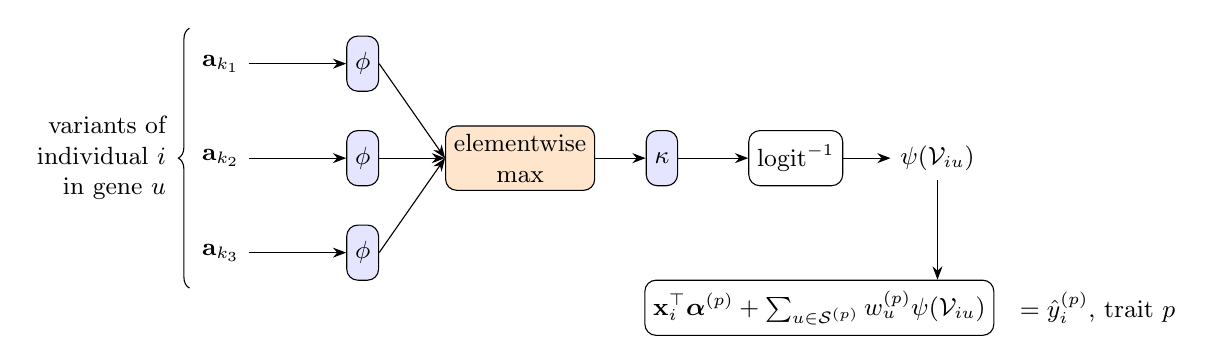
\begin{tikzpicture}[>=Stealth, every node/.style={font=\small},
      box/.style={draw, rounded corners, align=center, inner sep=3pt, minimum height=7mm}]
    \foreach \k/\y in {1/1.2, 2/0, 3/-1.2} {
      \node (a\k) at (0,\y) {$\va_{k_\k}$};
      \node[box, fill=blue!10] (p\k) at (1.8,\y) {$\phi$};
      \draw[->] (a\k) -- (p\k);
    }
    \node[box, fill=orange!20] (mx) at (3.8,0) {elementwise\\max};
    \foreach \k in {1,2,3} \draw[->] (p\k.east) -- (mx.west);
    \node[box, fill=blue!10] (rh) at (5.6,0) {$\kappa$};
    \node[box] (sg) at (7.3,0) {$\operatorname{logit}^{-1}$};
    \node (psi) at (9.1,0) {$\psi(\mathcal{V}_{iu})$};
    \draw[->] (mx) -- (rh); \draw[->] (rh) -- (sg); \draw[->] (sg) -- (psi);
    \node[box] (lin) at (7.6,-1.9) {$\vx_i^\top\valpha^{(p)}+\sum_{u\in\mathcal{S}^{(p)}}w_u^{(p)}\psi(\mathcal{V}_{iu})$};
    \draw[->] (psi) -- (psi |- lin.north);
    \node[right=2mm of lin] {$=\hat y_i^{(p)}$, trait $p$};
    \draw[decorate, decoration={brace, amplitude=4pt}] (-0.4,-1.65) -- (-0.4,1.65) node[midway, left=5pt, align=right] {variants of\\individual $i$\\in gene $u$};
  \end{tikzpicture}
  \caption{DeepRVAT. Each variant's annotations pass through a shared network $\phi$, the outputs are pooled by an elementwise maximum, and a second network $\kappa$ with a logistic output gives the gene impairment score $\psi$. During training, the scores of seed genes predict each trait through a linear model. After \citet{clarke2024}.}
  \label{fig:deeprvat}
\end{figure}

\subsection{Training and testing}

The score function is trained to predict traits. For trait $p$, with covariates $\vx_i$ (age, sex, genetic principal components) and coefficients $\valpha^{(p)}$, the prediction is
\begin{equation}
  \hat y_i^{(p)} = \vx_i^\top\valpha^{(p)} + \sum_{u\in\mathcal{S}^{(p)}} w_u^{(p)}\,\psi(\mathcal{V}_{iu}),
\end{equation}
where $\mathcal{S}^{(p)}$ is a set of \emph{seed genes} for trait $p$ and $w_u^{(p)}\in\R$ is a gene-specific coefficient. The networks $\phi$ and $\kappa$ are shared across all genes and all traits; only $\valpha^{(p)}$ and $w_u^{(p)}$ are specific to a trait. The loss is the squared error averaged over traits, minimized by stochastic gradient descent. The seed genes give the training signal. They were the genes significant in a conventional analysis that combines burden and SKAT tests of loss-of-function and missense variants with $\BetaD(1,25)$ weights. Training used 21 quantitative traits in about 160,000 exome-sequenced individuals from the UK Biobank. Sharing $\psi$ across traits means that what is learned about damaging variants from, say, lipid genes transfers to every other gene and trait. The score is ``trait-agnostic'', a learned, general-purpose definition of gene impairment.

For association testing, the trained $\psi$ is computed for every gene and individual and used as the burden score of Section~\ref{sec:burden}: for each gene $u$, the trait is regressed on $\psi(\mathcal{V}_{iu})$ and the covariates, and $H_0:\beta=0$ is tested with a score test. Genes outside the seed set can therefore be discovered. To avoid circularity, the model is trained with cross-validation: each individual's score is computed from models that were not trained on that individual. The seed genes themselves were chosen using the full data, so \citet{clarke2024} also checked the discoveries by replication in a larger UK Biobank release and on traits not used in training. Compared with burden and SKAT baselines, DeepRVAT found more significant gene-trait associations across the quantitative and binary traits it was applied to, and its scores improved the identification of individuals at high genetic risk.

DeepRVAT illustrates the trajectory of this chapter. A burden test hard-codes the prior that rare damaging variants matter; SKAT and the functional score test let the data choose among a few such priors; DeepRVAT learns the prior as a flexible function of annotations, with the statistical test kept simple so that its calibration is easy to check.

%======================================================================
\section{Summary}
%======================================================================

\begin{itemize}
  \item The power of a single-variant test depends on the sample size and MAF through approximately $Nf$, so rare variants need very large samples and de novo mutations cannot be tested individually. Rare variants can still have large effects, because selection keeps damaging variants rare.
  \item Burden tests aggregate the variants in a gene into a single score. They are powerful when most qualifying variants are causal with effects in the same direction, and depend on choices of frequency threshold, functional filter, controls and quality control. De novo mutations are tested against a mutation-rate model that accounts for sequence context such as CpG sites.
  \item Pathogenicity predictors include conservation scores, supervised and unsupervised combinations of annotations, and sequence models. LINSIGHT learns from the patterns of divergence and polymorphism that natural selection produces, with the prior probability of selection modelled as a function of genomic features.
  \item SKAT treats per-variant effects as random with mean zero and tests their variance component with a score statistic $\sum_jw_j^2S_j^2$ whose null distribution is a mixture of $\chi^2_1$ variables. It is robust to mixed effect directions. SKAT-O combines SKAT and burden through a correlation parameter $\rho$ and the minimum p-value over a grid.
  \item The functional score test adds one variance component per annotation and combines the resulting statistics, gaining power when annotations are informative and losing little when they are not.
  \item In autism, de novo noncoding mutations scored with deep learning sequence models and a classifier trained on known disease mutations have higher predicted impact in probands than in siblings. Network differential enrichment pools sparse mutations across functionally related genes, implicating synaptic and chromatin regulation genes. Reporter assays confirm that prioritized mutations alter regulatory activity.
  \item RNA-seq from patients reveals the consequences of rare variants as expression, splicing or allelic outliers, judged against a reference population, and ANEVA-DOT calibrates allelic imbalance by each gene's tolerance of regulatory variation.
  \item DeepRVAT learns a gene impairment score from variant annotations with a deep set network trained across traits, and uses it as the burden score in a conventional test.
\end{itemize}

%======================================================================
\section*{Exercises}
%======================================================================

\begin{enumerate}
  \item Using~\eqref{eq:ncp}, find the sample size needed for 80\% power at $\alpha=5\times10^{-8}$ to detect a variant with $f=10^{-3}$ and $\beta=0.25\sigma$. How does the answer change if the variant is ten times rarer?
  \item Starting from the marginal likelihood $\vy\sim\Normal(\mX\valpha,\sigma^2\mI+\tau\mG\mW\mR_\rho\mW\mG^\top)$, derive the score statistic~\eqref{eq:skat_q} and show that it equals $(1-\rho)Q_{\text{SKAT}}+\rho Q_{\text{burden}}$.
  \item Suppose a region has $M$ independent variants with equal weights and equal frequencies, half with effect $+\beta$ and half with effect $-\beta$. Show that the expected burden score statistic $\E[\vw^\top\vS]$ is zero under the alternative, while $\E[Q_{\text{SKAT}}]$ increases with $\beta^2$.
  \item For the simplified LINSIGHT likelihood~\eqref{eq:linsight_lik}, derive the gradient of $\log P(X_i)$ with respect to $\vw_\rho$, for the Gompertz link $g(x)=\exp(-3e^{-x})$. Show that sites with the pattern $\mathsf{D}$ always push $\rho_i$ down, and explain why monomorphic sites push it up only slightly.
  \item Show that the effective sample size $N=(\sum_ma_m)^2/\sum_ma_m^2$ satisfies $1\leq N\leq n$ for $n$ positive weights, with equality at the upper end only when all weights are equal.
  \item In the ANEVA-DOT model, show that without overdispersion ($c\to\infty$) and with $V^G\to 0$, the test reduces to a binomial test of $r$ against $n/2$. Why does this test flag far too many genes in practice?
  \item Explain why the elementwise maximum in~\eqref{eq:deeprvat} makes $\psi$ invariant to the order of the variants. Construct an example in which replacing the maximum by a sum would make a gene with many benign variants look more impaired than a gene with one damaging variant.
\end{enumerate}

\bibliographystyle{abbrvnat}
\bibliography{chapter13}
\end{document}
